\documentclass[]{book}
\usepackage{lmodern}
\usepackage{amssymb,amsmath}
\usepackage{ifxetex,ifluatex}
\usepackage{fixltx2e} % provides \textsubscript
\ifnum 0\ifxetex 1\fi\ifluatex 1\fi=0 % if pdftex
  \usepackage[T1]{fontenc}
  \usepackage[utf8]{inputenc}
\else % if luatex or xelatex
  \ifxetex
    \usepackage{mathspec}
  \else
    \usepackage{fontspec}
  \fi
  \defaultfontfeatures{Ligatures=TeX,Scale=MatchLowercase}
\fi
% use upquote if available, for straight quotes in verbatim environments
\IfFileExists{upquote.sty}{\usepackage{upquote}}{}
% use microtype if available
\IfFileExists{microtype.sty}{%
\usepackage{microtype}
\UseMicrotypeSet[protrusion]{basicmath} % disable protrusion for tt fonts
}{}
\usepackage[margin=1in]{geometry}
\usepackage{hyperref}
\hypersetup{unicode=true,
            pdftitle={Methods in Macroecology and Macroevolution},
            pdfauthor={Natalie Cooper (natalie.cooper@nhm.ac.uk)},
            pdfborder={0 0 0},
            breaklinks=true}
\urlstyle{same}  % don't use monospace font for urls
\usepackage{natbib}
\bibliographystyle{plainnat}
\usepackage{color}
\usepackage{fancyvrb}
\newcommand{\VerbBar}{|}
\newcommand{\VERB}{\Verb[commandchars=\\\{\}]}
\DefineVerbatimEnvironment{Highlighting}{Verbatim}{commandchars=\\\{\}}
% Add ',fontsize=\small' for more characters per line
\usepackage{framed}
\definecolor{shadecolor}{RGB}{248,248,248}
\newenvironment{Shaded}{\begin{snugshade}}{\end{snugshade}}
\newcommand{\KeywordTok}[1]{\textcolor[rgb]{0.13,0.29,0.53}{\textbf{{#1}}}}
\newcommand{\DataTypeTok}[1]{\textcolor[rgb]{0.13,0.29,0.53}{{#1}}}
\newcommand{\DecValTok}[1]{\textcolor[rgb]{0.00,0.00,0.81}{{#1}}}
\newcommand{\BaseNTok}[1]{\textcolor[rgb]{0.00,0.00,0.81}{{#1}}}
\newcommand{\FloatTok}[1]{\textcolor[rgb]{0.00,0.00,0.81}{{#1}}}
\newcommand{\ConstantTok}[1]{\textcolor[rgb]{0.00,0.00,0.00}{{#1}}}
\newcommand{\CharTok}[1]{\textcolor[rgb]{0.31,0.60,0.02}{{#1}}}
\newcommand{\SpecialCharTok}[1]{\textcolor[rgb]{0.00,0.00,0.00}{{#1}}}
\newcommand{\StringTok}[1]{\textcolor[rgb]{0.31,0.60,0.02}{{#1}}}
\newcommand{\VerbatimStringTok}[1]{\textcolor[rgb]{0.31,0.60,0.02}{{#1}}}
\newcommand{\SpecialStringTok}[1]{\textcolor[rgb]{0.31,0.60,0.02}{{#1}}}
\newcommand{\ImportTok}[1]{{#1}}
\newcommand{\CommentTok}[1]{\textcolor[rgb]{0.56,0.35,0.01}{\textit{{#1}}}}
\newcommand{\DocumentationTok}[1]{\textcolor[rgb]{0.56,0.35,0.01}{\textbf{\textit{{#1}}}}}
\newcommand{\AnnotationTok}[1]{\textcolor[rgb]{0.56,0.35,0.01}{\textbf{\textit{{#1}}}}}
\newcommand{\CommentVarTok}[1]{\textcolor[rgb]{0.56,0.35,0.01}{\textbf{\textit{{#1}}}}}
\newcommand{\OtherTok}[1]{\textcolor[rgb]{0.56,0.35,0.01}{{#1}}}
\newcommand{\FunctionTok}[1]{\textcolor[rgb]{0.00,0.00,0.00}{{#1}}}
\newcommand{\VariableTok}[1]{\textcolor[rgb]{0.00,0.00,0.00}{{#1}}}
\newcommand{\ControlFlowTok}[1]{\textcolor[rgb]{0.13,0.29,0.53}{\textbf{{#1}}}}
\newcommand{\OperatorTok}[1]{\textcolor[rgb]{0.81,0.36,0.00}{\textbf{{#1}}}}
\newcommand{\BuiltInTok}[1]{{#1}}
\newcommand{\ExtensionTok}[1]{{#1}}
\newcommand{\PreprocessorTok}[1]{\textcolor[rgb]{0.56,0.35,0.01}{\textit{{#1}}}}
\newcommand{\AttributeTok}[1]{\textcolor[rgb]{0.77,0.63,0.00}{{#1}}}
\newcommand{\RegionMarkerTok}[1]{{#1}}
\newcommand{\InformationTok}[1]{\textcolor[rgb]{0.56,0.35,0.01}{\textbf{\textit{{#1}}}}}
\newcommand{\WarningTok}[1]{\textcolor[rgb]{0.56,0.35,0.01}{\textbf{\textit{{#1}}}}}
\newcommand{\AlertTok}[1]{\textcolor[rgb]{0.94,0.16,0.16}{{#1}}}
\newcommand{\ErrorTok}[1]{\textcolor[rgb]{0.64,0.00,0.00}{\textbf{{#1}}}}
\newcommand{\NormalTok}[1]{{#1}}
\usepackage{longtable,booktabs}
\usepackage{graphicx,grffile}
\makeatletter
\def\maxwidth{\ifdim\Gin@nat@width>\linewidth\linewidth\else\Gin@nat@width\fi}
\def\maxheight{\ifdim\Gin@nat@height>\textheight\textheight\else\Gin@nat@height\fi}
\makeatother
% Scale images if necessary, so that they will not overflow the page
% margins by default, and it is still possible to overwrite the defaults
% using explicit options in \includegraphics[width, height, ...]{}
\setkeys{Gin}{width=\maxwidth,height=\maxheight,keepaspectratio}
\IfFileExists{parskip.sty}{%
\usepackage{parskip}
}{% else
\setlength{\parindent}{0pt}
\setlength{\parskip}{6pt plus 2pt minus 1pt}
}
\setlength{\emergencystretch}{3em}  % prevent overfull lines
\providecommand{\tightlist}{%
  \setlength{\itemsep}{0pt}\setlength{\parskip}{0pt}}
\setcounter{secnumdepth}{5}
% Redefines (sub)paragraphs to behave more like sections
\ifx\paragraph\undefined\else
\let\oldparagraph\paragraph
\renewcommand{\paragraph}[1]{\oldparagraph{#1}\mbox{}}
\fi
\ifx\subparagraph\undefined\else
\let\oldsubparagraph\subparagraph
\renewcommand{\subparagraph}[1]{\oldsubparagraph{#1}\mbox{}}
\fi

%%% Use protect on footnotes to avoid problems with footnotes in titles
\let\rmarkdownfootnote\footnote%
\def\footnote{\protect\rmarkdownfootnote}

%%% Change title format to be more compact
\usepackage{titling}

% Create subtitle command for use in maketitle
\newcommand{\subtitle}[1]{
  \posttitle{
    \begin{center}\large#1\end{center}
    }
}

\setlength{\droptitle}{-2em}
  \title{Methods in Macroecology and Macroevolution}
  \pretitle{\vspace{\droptitle}\centering\huge}
  \posttitle{\par}
  \author{Natalie Cooper
(\href{mailto:natalie.cooper@nhm.ac.uk}{\nolinkurl{natalie.cooper@nhm.ac.uk}})}
  \preauthor{\centering\large\emph}
  \postauthor{\par}
  \predate{\centering\large\emph}
  \postdate{\par}
  \date{February 2017}

\usepackage{booktabs}

\begin{document}
\maketitle

{
\setcounter{tocdepth}{1}
\tableofcontents
}
\chapter{Methods in Macroecology and Macroevolution: Module
outline}\label{methods-in-macroecology-and-macroevolution-module-outline}

\section{Module Aims}\label{module-aims}

The aim of this module is to introduce you to some of the cutting-edge
methods being used in macroecology and macroevolution, with particular
focus on work being done right now at the Museum. Rather than
concentrating on learning theory through lectures, the module will
introduce you to various ways we collect, analyse and interpret
macro-scale data with a large emphasis on practical work, mostly using
R.

\section{Datasets and practical
handouts}\label{datasets-and-practical-handouts}

All datasets and practical handouts are available on GitHub. It can be
tricky to download data from GitHub if you don't know what you're doing
and/or don't want to clone the entire repository so the materials are
also available at this DropBox link: {[}{]}. It will save time if you
download this before coming to class.

\section{Timetable}\label{timetable}

There will be one morning and one afternoon session each day. Morning
sessions will run from 10am-1pm, afternoon sessions from 2pm-5pm. Not
every session will require a full three hours. Instructors for each
session are below. Note that Thursday and Friday of the first week we
have had to move to the Gavin de Beer room. \textbf{PLEASE BRING
LAPTOPS}.

\textbf{Thursday 23rd February - GAVIN DE BEER not UBR or LBR}

\begin{itemize}
\item
  Morning: What are macroecology and macroevolution? Introduction to the
  module, assessments, and aims. \emph{Natalie Cooper
  (\href{mailto:natalie.cooper@nhm.ac.uk}{\nolinkurl{natalie.cooper@nhm.ac.uk}})}
\item
  Afternoon: Macroecology I: Macroecological patterns and diversity
  indices in R. \emph{Natalie Cooper
  (\href{mailto:natalie.cooper@nhm.ac.uk}{\nolinkurl{natalie.cooper@nhm.ac.uk}})}
\end{itemize}

\textbf{Friday February 24th February - GAVIN DE BEER not UBR or LBR}

\begin{itemize}
\item
  Morning: Big Data I: Using Big Data in conservation with the PREDICTS
  project. \emph{Andy Purvis
  (\href{mailto:a.purvis@nhm.ac.uk}{\nolinkurl{a.purvis@nhm.ac.uk}})}
\item
  Afternoon: Big data II: Using the paleobiology database (PBDB) to get
  data on fossil species for macroecological and macroevolutionary
  analyses. \emph{Terri Cleary
  (\href{mailto:t.cleary@nhm.ac.uk}{\nolinkurl{t.cleary@nhm.ac.uk}})}
\end{itemize}

\textbf{Monday February 27th February - UBR/LBR }

\begin{itemize}
\item
  Morning: Comparative Biology: The comparative method, dealing with
  phylogenetic non-independence in comparative analyses. PGLS in R.
  \emph{Natalie Cooper
  (\href{mailto:natalie.cooper@nhm.ac.uk}{\nolinkurl{natalie.cooper@nhm.ac.uk}})}
\item
  Afternoon: Macroevolution I: Macroevolutionary patterns and models of
  evolution in R. \emph{Natalie Cooper
  (\href{mailto:natalie.cooper@nhm.ac.uk}{\nolinkurl{natalie.cooper@nhm.ac.uk}})}
\end{itemize}

\textbf{Tuesday 28th February - UBR/LBR}

\begin{itemize}
\item
  Morning: Big data III: Using museum specimen data in macroecological
  and macroevolutionary analyses. Geometric morphometrics. \emph{Natalie
  Cooper
  (\href{mailto:natalie.cooper@nhm.ac.uk}{\nolinkurl{natalie.cooper@nhm.ac.uk}})}
\item
  Afternoon: Macroevolution II: case study using Foraminifera.
  \emph{Isabel Fenton
  (\href{mailto:i.fenton@nhm.ac.uk}{\nolinkurl{i.fenton@nhm.ac.uk}})}
\end{itemize}

\textbf{Wednesday 1st March - UBR/LBR}

\begin{itemize}
\item
  Morning: Macroevolution III: Diversification rates and adaptive
  radiations. \emph{Natalie Cooper
  (\href{mailto:natalie.cooper@nhm.ac.uk}{\nolinkurl{natalie.cooper@nhm.ac.uk}})}
\item
  Afternoon: Critical thinking: Do you trust your methods? \emph{Natalie
  Cooper
  (\href{mailto:natalie.cooper@nhm.ac.uk}{\nolinkurl{natalie.cooper@nhm.ac.uk}})}
\end{itemize}

\textbf{Thursday 2nd March AND Friday 3rd March - UBR}

\emph{Richard Twitchett
(\href{mailto:r.twitchett@nhm.ac.uk}{\nolinkurl{r.twitchett@nhm.ac.uk}})}

\begin{itemize}
\tightlist
\item
  All day: Using fossil assemblages to assess the impact of mass
  extinction events: comparative palaeoecology of Ordovician and
  Silurian fossil assemblages (practical and assessment).
\end{itemize}

\section{Assessment}\label{assessment}

There are two assessments connected to this module.

The first will be based on computer practicals early in the course.
These will be done at the end of the practicals, and consist of some
online multiple choice questions. No write up will be required and the
assessment will be completed by the end of the week, if not the end of
the practical.

The second, although within this module, belongs to the Paleobiology
module. Due to the large class size during that module it couldn't
happen there so we've moved it here. However, the techniques and
concepts are highly relevant to macroecology and macroevolution. Richard
Twitchett
(\href{mailto:r.twitchett@nhm.ac.uk}{\nolinkurl{r.twitchett@nhm.ac.uk}})
will provide a full explanation of the assessment during the practical
on \textbf{Thursday 2nd March and Friday 3rd March}.

\chapter{What you need to be able to do in R before you
start}\label{what-you-need-to-be-able-to-do-in-r-before-you-start}

Most people taking this module have used R a lot already, but it is
possible you're a bit rusty, or you've found this course on GitHub and
have no R experience. This isn't a problem, I will try and summarise
what you need to be able to do to get these practicals running below.
However, I'm not going to write a help guide to R here, if you can't
work out how to open it and get started etc. I strongly recommend the
book \href{http://www.r4all.org/}{Getting Started With R} or there are
lots of great tutorials online.

Throughout, R code will be in shaded boxes:

\begin{Shaded}
\begin{Highlighting}[]
\KeywordTok{library}\NormalTok{(ape)}
\end{Highlighting}
\end{Shaded}

R output will be preceded by \#\# and important comments will be in
quote blocks:

Note that many things in R can be done in multiple ways. You should
choose the methods you feel most comfortable with, and do not panic if
someone is doing the same analyses as you in a different way!

\section{Installing R (and RStudio)}\label{installing-r-and-rstudio}

\begin{itemize}
\tightlist
\item
  Install R from {[}\url{https://cran.r-project.org}{]}
\item
  You can install RStudio from
  {[}\url{http://www.rstudio.com/products/rstudio/download/}{]}. I'd
  recommend trying this out if you're a beginner as it has a nicer
  interface.
\end{itemize}

\section{Setting the working
directory}\label{setting-the-working-directory}

To use the practicals you need to download all the files for each
practical into a folder somewhere on your computer (I usually put mine
on the Desktop). We will then tell R to look in this folder for all data
etc. by \textbf{setting the working directory} to that folder.

To set the working directory you'll need to know what the \textbf{path}
of the folder is. The path is really easy to find in a Windows machine,
just click on the address bar of the folder and the whole path will
appear. For example on my Windows machine, the path is:

\begin{Shaded}
\begin{Highlighting}[]
\NormalTok{C:}\ErrorTok{/}\NormalTok{Users/Natalie/Desktop/RAnalyses}
\end{Highlighting}
\end{Shaded}

It's a bit trickier to find the path on a Mac, so use Google if you need
help. On my Mac the path is:

\begin{Shaded}
\begin{Highlighting}[]
\NormalTok{~}\ErrorTok{/}\NormalTok{Desktop/RAnalyses}
\end{Highlighting}
\end{Shaded}

Note that the tilde \textasciitilde{} is a shorthand for /Users/Natalie.

We can then set the working directory to your folder using
\texttt{setwd}:

\begin{Shaded}
\begin{Highlighting}[]
\KeywordTok{setwd}\NormalTok{(}\StringTok{"~/Desktop/RAnalyses"}\NormalTok{)}
\end{Highlighting}
\end{Shaded}

Alternatively if using RStudio you use the menus to do this. Go to
Session \textgreater{} Set Working Directory \textgreater{} Choose
Directory.

Setting the working directory tells R which folder to look for data in
(and which folder you'd like it to write results to). It saves a bit of
typing when reading files into R. Now I can read in a file called
\texttt{mydata.csv} as follows:

\begin{Shaded}
\begin{Highlighting}[]
\NormalTok{mydata <-}\StringTok{ }\KeywordTok{read.csv}\NormalTok{(}\StringTok{"mydata.csv"}\NormalTok{)}
\end{Highlighting}
\end{Shaded}

rather than having to specify the folder too:

\begin{Shaded}
\begin{Highlighting}[]
\NormalTok{mydata <-}\StringTok{ }\KeywordTok{read.csv}\NormalTok{(}\StringTok{"~/Desktop/RAnalyses/mydata.csv"}\NormalTok{)}
\end{Highlighting}
\end{Shaded}

\begin{quote}
Remember if you move the data files, or the folder itself, you'll need
to set the working directory again.
\end{quote}

\section{Using a script}\label{using-a-script}

Next, open a text editor. R has an inbuilt editor that works pretty
well, but NotePad and TextEdit are fine too. However, I \textbf{highly}
recommend using something that will highlight code for you. My personal
favorite is Sublime Text 2, because you can also use it for any other
kind of text editing like LaTeX, html etc. RStudio's editor is also very
nice.

You should type (or copy and paste) your code into the text editor, edit
it until you think it'll work, and then either paste it into R's console
window, or you can highlight the bit of code you want to run and press
\texttt{ctrl} or \texttt{cmd} and \texttt{enter} or \texttt{R}
(different computers seem to do this differently). This will
automatically send it to the console.

Saving the script file lets you keep a record of the code you used,
which can be a great time saver if you want to use it again, especially
as you know this code will work!

\textbf{You can cut and paste code from my handouts into your script.
You don't need to retype everything!}

If you want to add comments to the file (i.e., notes to remind yourself
what the code is doing), put a hash/pound sign (\#) in front of the
comment.

\begin{Shaded}
\begin{Highlighting}[]
\CommentTok{# Comments are ignored by R but remind you what the code is doing. }
\CommentTok{# You need a # at the start of each line of a comment.}
\CommentTok{# Always make plenty of notes to help you remember what you did and why}
\end{Highlighting}
\end{Shaded}

\section{Installing and loading extra packages in
R}\label{installing-and-loading-extra-packages-in-r}

To run any specialised analysis in R, you need to download one or more
additional packages from the basic R installation. For these problem
sets you will need to install the following packages:

\begin{itemize}
\tightlist
\item
  \texttt{ape}
\item
  \texttt{geiger}
\item
  \texttt{picante}
\item
  \texttt{caper}
\item
  \texttt{BAMMtools}
\end{itemize}

To install the package \texttt{ape}:

\begin{Shaded}
\begin{Highlighting}[]
\KeywordTok{install.packages}\NormalTok{(}\StringTok{"ape"}\NormalTok{)}
\end{Highlighting}
\end{Shaded}

Pick the closest mirror to you if asked.

You've \emph{installed} the packages but they don't automatically get
loaded into your R session. Instead you need to tell R to load them
\textbf{every time} you start a new R session and want to use functions
from these packages. To load the package \texttt{ape} into your current
R session:

\begin{Shaded}
\begin{Highlighting}[]
\KeywordTok{library}\NormalTok{(ape)}
\end{Highlighting}
\end{Shaded}

You can think of \texttt{install.packages} like installing an app from
the App Store on your smart phone - \emph{you only do this once} - and
\texttt{library} as being like pushing the app button on your phone -
\emph{you do this every time you want to use the app}.

\section{Loading and viewing your data in
R}\label{loading-and-viewing-your-data-in-r}

R can read files in lots of formats, including comma-delimited and
tab-delimited files. Excel (and many other applications) can output
files in this format (it's an option in the \texttt{Save\ As} dialog box
under the \texttt{File} menu). Mostly I will give you .csv or .txt files
during these practicals. As an example, here is how you would read in
the tab-delimited text file called \texttt{Primatedata.txt} which we are
going to use in the PGLS practical. Load these data as follows, assuming
you have set your working directory (see step 2 above).

\begin{Shaded}
\begin{Highlighting}[]
\NormalTok{primatedata <-}\StringTok{ }\KeywordTok{read.delim}\NormalTok{(}\StringTok{"Primatedata.txt"}\NormalTok{, }\DataTypeTok{header =} \OtherTok{TRUE}\NormalTok{)}
\end{Highlighting}
\end{Shaded}

You can use \texttt{read.delim} for tab delimited files or
\texttt{read.csv} for comma delimited files. \texttt{header\ =\ TRUE},
indicates that the first line of the data contains column headings.

This is a good point to note that unless you \_\_tell\_\_R you want to
do something, it won't do it automatically. So here if you successfully
entered the data, R won't give you any indication that it worked.
Instead you need to specifically ask R to look at the data.

We can look at the data by typing:

\begin{Shaded}
\begin{Highlighting}[]
\KeywordTok{str}\NormalTok{(primatedata)}
\end{Highlighting}
\end{Shaded}

\begin{verbatim}
## 'data.frame':    77 obs. of  8 variables:
##  $ Order          : Factor w/ 1 level "Primates": 1 1 1 1 1 1 1 1 1 1 ...
##  $ Family         : Factor w/ 15 levels "Aotidae","Atelidae",..: 2 2 2 14 3 3 3 4 4 4 ...
##  $ Binomial       : Factor w/ 77 levels "Alouatta palliata",..: 5 6 7 8 9 10 11 15 16 17 ...
##  $ AdultBodyMass_g: num  6692 7582 8697 958 558 ...
##  $ GestationLen_d : num  138 226 228 164 154 ...
##  $ HomeRange_km2  : num  2.28 0.73 1.36 0.02 0.32 0.02 0.00212 0.51 0.16 0.24 ...
##  $ MaxLongevity_m : num  336 328 454 304 215 ...
##  $ SocialGroupSize: num  14.5 42 20 2.95 6.85 ...
\end{verbatim}

\textbf{Always} look at your data before beginning any analysis to check
it read in correctly.

\texttt{str} shows the structure of the data frame (this can be a really
useful command when you have a big data file). It also tells you what
kind of variables R thinks you have (characters, integers, numeric,
factors etc.). Some R functions need the data to be certain kinds of
variables so it's useful to check this.

As you can see, the data contains the following variables: Order,
Family, Binomial, AdultBodyMass\_g, GestationLen\_d, HomeRange\_km2,
MaxLongevity\_m, and SocialGroupSize.

\begin{Shaded}
\begin{Highlighting}[]
\KeywordTok{head}\NormalTok{(primatedata)}
\end{Highlighting}
\end{Shaded}

\begin{verbatim}
##      Order      Family           Binomial AdultBodyMass_g GestationLen_d
## 1 Primates    Atelidae   Ateles belzebuth         6692.42         138.20
## 2 Primates    Atelidae   Ateles geoffroyi         7582.40         226.37
## 3 Primates    Atelidae    Ateles paniscus         8697.25         228.18
## 4 Primates Pitheciidae  Callicebus moloch          958.13         164.00
## 5 Primates     Cebidae  Callimico goeldii          558.00         153.99
## 6 Primates     Cebidae Callithrix jacchus          290.21         144.00
##   HomeRange_km2 MaxLongevity_m SocialGroupSize
## 1          2.28          336.0           14.50
## 2          0.73          327.6           42.00
## 3          1.36          453.6           20.00
## 4          0.02          303.6            2.95
## 5          0.32          214.8            6.85
## 6          0.02          201.6            8.55
\end{verbatim}

This gives you the first few rows of data along with the column
headings.

\begin{Shaded}
\begin{Highlighting}[]
\KeywordTok{names}\NormalTok{(primatedata)}
\end{Highlighting}
\end{Shaded}

\begin{verbatim}
## [1] "Order"           "Family"          "Binomial"        "AdultBodyMass_g"
## [5] "GestationLen_d"  "HomeRange_km2"   "MaxLongevity_m"  "SocialGroupSize"
\end{verbatim}

This gives you the names of the columns.

\begin{Shaded}
\begin{Highlighting}[]
\NormalTok{primatedata}
\end{Highlighting}
\end{Shaded}

This will print out all of the data!

\emph{This should be everything you need to know to get the practicals
that follow working. Let me know if you have any problems
(\href{mailto:natalie.cooper@nhm.ac.uk}{\nolinkurl{natalie.cooper@nhm.ac.uk}}).}

\chapter{Diversity Indices in R}\label{diversity-indices-in-r}

The aims of this practical are to learn how to use R to estimate
diversity indices and species accumulation curves. You will need some of
these functions to complete your paleoecology assessment.

We will be using some made up data about Pokemon sightings within the
Museum.

\textbf{REMEMBER}

\begin{itemize}
\tightlist
\item
  Download all of the data for the practical into a folder somewhere on
  your computer.
\item
  Set your working directory to this folder.
\item
  Start a new script for this practical.
\end{itemize}

You will also need to install the following packages:

\begin{itemize}
\tightlist
\item
  \texttt{vegan}
\item
  \texttt{picante}
\end{itemize}

\begin{center}\rule{0.5\linewidth}{\linethickness}\end{center}

\section{What are diversity indices?}\label{what-are-diversity-indices}

A diversity index is a measure of the ``diversity'' of an area.
\emph{Diversity} could be measured in terms of the numbers of species
(or higher taxonomic groupings like genera, families, phyla), or other
metrics such as number of haplotypes if you're interested in genetic
diversity, or number of functional groups for studies of functional
diversity.

Many diversity indices also account for how evenly spread these
different types are. For example, they identify whether there are there
five species with 10 individuals of each (even), or five species with
one species with 96 individuals and four species with one individual
each (uneven). These differences in evenness may be as important for
ecosystem function as the number of species.

There are about a million different diversity indices (OK this is a
slight exaggeration but there are a lot check out the
\href{https://cran.r-project.org/web/packages/vegan/vegan.pdf}{vegan
package} vignette and search for ``diversity''), and different people
prefer different measures for different questions. Amusingly the
\texttt{vegan} helpfile for the function \texttt{diversify} states
``these indices are all very closely related (Hill 1973), and there is
no reason to despise one more than others (but if you are a graduate
student, don't drag me in, but obey your Professor's orders)''.

\subsection{\texorpdfstring{\(\alpha\), \(\beta\) and \(\gamma\)
diversity (Whittaker 1960,
1972)}{\textbackslash{}alpha, \textbackslash{}beta and \textbackslash{}gamma diversity (Whittaker 1960, 1972)}}\label{alpha-beta-and-gamma-diversity-whittaker-1960-1972}

\begin{itemize}
\tightlist
\item
  \(\alpha\) diversity is the mean species diversity in sites or
  habitats at a local scale.
\item
  \(\beta\) diversity is turnover in \(\alpha\) diversity among
  different sites.
\item
  \(\gamma\) gamma diversity is diversity at the landscape level.
\end{itemize}

For example, if we count the species in Hyde Park and Green Park, we'd
have a measure of \(\alpha\) diversity for each. \(\beta\) diversity
would measure the difference between species found in Hyde Park and
those found in Green Park. \(\gamma\) diversity would be all the species
found across London.

\(\beta\) diversity is the hardest to measure, and there are far more
metrics for measuring this than any others.

\section{Practical example using
Pokemon\ldots{}}\label{practical-example-using-pokemon}

We're going to play around with some invented data on sampling sites
within the Museum and the Pokemon we've managed to find there (don't
complain about my unlikely Pokemon combinations, they're just made up
data with Pokemon names rather than A, B, C etc!).

\begin{figure}
\centering

\includegraphics{pokemon.png}
\caption{Who doesn't love a practical handout being interrupted by an
enormous Pikachu?}
\end{figure}

\begin{Shaded}
\begin{Highlighting}[]
\CommentTok{# Load picante and vegan}
\KeywordTok{library}\NormalTok{(picante)}
\KeywordTok{library}\NormalTok{(vegan)}
\end{Highlighting}
\end{Shaded}

Next read in the data and take a look at it.

\begin{Shaded}
\begin{Highlighting}[]
\NormalTok{pokemon <-}\StringTok{ }\KeywordTok{read.csv}\NormalTok{(}\StringTok{"pokemon_communities.csv"}\NormalTok{)}
\end{Highlighting}
\end{Shaded}

\begin{Shaded}
\begin{Highlighting}[]
\CommentTok{# Look at the data}
\NormalTok{pokemon}
\end{Highlighting}
\end{Shaded}

For the \texttt{vegan} functions to work you need a matrix where the
columns are the species names, the rows are the communities, and the
contents of the matrix are the numbers of each species found at each
site (or presence absence data as 0s and 1s). We can use the
\texttt{sample2matrix} function in \texttt{picante} to do this easily.

Note that this only works if your first variable is the name of the
site, your second is abundance and your third is the names of the
species present.

\begin{Shaded}
\begin{Highlighting}[]
\NormalTok{pokemon.matrix <-}\StringTok{ }\KeywordTok{sample2matrix}\NormalTok{(pokemon)}

\CommentTok{# Look at the matrix}
\NormalTok{pokemon.matrix}
\end{Highlighting}
\end{Shaded}

\begin{verbatim}
##        Bulbasaur Caterpie Charmander Pidgey Pikachu Psyduck Rattata
## site01         5        0          3      0       0       0       0
## site02         0        0          0      6       0       0       6
## site03         1        0          1      1       1       0      10
## site04         0        0          2      0       1       0       0
## site05         0        2          0      4       0       0       3
## site06         0        0          0      0       0       1       0
## site07         3        3          3      3       0       0       3
## site08         5        5          0      0       0       0       0
## site09         0        0          0      0       0       0       0
## site10         0        0          6      3       0       0       0
##        Spearow Squirtle Zubat
## site01       0        0     0
## site02       1        0     0
## site03       1        0     0
## site04       0        0     0
## site05       0        3     0
## site06       0        0     0
## site07       3        3     0
## site08       0        0     0
## site09       0       10     0
## site10       0        0     2
\end{verbatim}

\section{Species diversity indices}\label{species-diversity-indices}

\subsection{\texorpdfstring{\(\alpha\)
diversity}{\textbackslash{}alpha diversity}}\label{alpha-diversity}

The simplest measure of \(\alpha\) diversity is just the number of
species in each site. You can easily extract this as follows.

\begin{Shaded}
\begin{Highlighting}[]
\KeywordTok{specnumber}\NormalTok{(pokemon.matrix)}
\end{Highlighting}
\end{Shaded}

\begin{verbatim}
## site01 site02 site03 site04 site05 site06 site07 site08 site09 site10 
##      2      3      6      2      4      1      7      2      1      3
\end{verbatim}

Simpson's and Shannon's diversity indices can be estimated using the
function \texttt{diversity}.

\begin{Shaded}
\begin{Highlighting}[]
\CommentTok{# Simpson's index}
\KeywordTok{diversity}\NormalTok{(pokemon.matrix, }\DataTypeTok{index =} \StringTok{"simpson"}\NormalTok{)}
\end{Highlighting}
\end{Shaded}

\begin{verbatim}
##    site01    site02    site03    site04    site05    site06    site07 
## 0.4687500 0.5680473 0.5333333 0.4444444 0.7361111 0.0000000 0.8571429 
##    site08    site09    site10 
## 0.5000000 0.0000000 0.5950413
\end{verbatim}

\begin{Shaded}
\begin{Highlighting}[]
\CommentTok{# Shannon's index}
\KeywordTok{diversity}\NormalTok{(pokemon.matrix, }\DataTypeTok{index =} \StringTok{"shannon"}\NormalTok{)}
\end{Highlighting}
\end{Shaded}

\begin{verbatim}
##    site01    site02    site03    site04    site05    site06    site07 
## 0.6615632 0.9110175 1.1729935 0.6365142 1.3579779 0.0000000 1.9459101 
##    site08    site09    site10 
## 0.6931472 0.0000000 0.9949236
\end{verbatim}

\subsection{\texorpdfstring{\(\beta\)
diversity}{\textbackslash{}beta diversity}}\label{beta-diversity}

The function \texttt{betadiver} allows you to estimate all the \(\beta\)
diversity indices mentioned in Koleff et al. 2003. For help on which
indices are included type:

\begin{Shaded}
\begin{Highlighting}[]
\KeywordTok{betadiver}\NormalTok{(}\DataTypeTok{help=}\OtherTok{TRUE}\NormalTok{)}
\end{Highlighting}
\end{Shaded}

\begin{verbatim}
## 1 "w" = (b+c)/(2*a+b+c)
## 2 "-1" = (b+c)/(2*a+b+c)
## 3 "c" = (b+c)/2
## 4 "wb" = b+c
## 5 "r" = 2*b*c/((a+b+c)^2-2*b*c)
## 6 "I" = log(2*a+b+c) - 2*a*log(2)/(2*a+b+c) - ((a+b)*log(a+b) +
## (a+c)*log(a+c)) / (2*a+b+c)
## 7 "e" = exp(log(2*a+b+c) - 2*a*log(2)/(2*a+b+c) - ((a+b)*log(a+b)
## + (a+c)*log(a+c)) / (2*a+b+c))-1
## 8 "t" = (b+c)/(2*a+b+c)
## 9 "me" = (b+c)/(2*a+b+c)
## 10 "j" = a/(a+b+c)
## 11 "sor" = 2*a/(2*a+b+c)
## 12 "m" = (2*a+b+c)*(b+c)/(a+b+c)
## 13 "-2" = pmin(b,c)/(pmax(b,c)+a)
## 14 "co" = (a*c+a*b+2*b*c)/(2*(a+b)*(a+c))
## 15 "cc" = (b+c)/(a+b+c)
## 16 "g" = (b+c)/(a+b+c)
## 17 "-3" = pmin(b,c)/(a+b+c)
## 18 "l" = (b+c)/2
## 19 "19" = 2*(b*c+1)/(a+b+c)/(a+b+c-1)
## 20 "hk" = (b+c)/(2*a+b+c)
## 21 "rlb" = a/(a+c)
## 22 "sim" = pmin(b,c)/(pmin(b,c)+a)
## 23 "gl" = 2*abs(b-c)/(2*a+b+c)
## 24 "z" = (log(2)-log(2*a+b+c)+log(a+b+c))/log(2)
\end{verbatim}

Note that some of these are similarity indices, and some are
dissimilarity indices. See Koleff et al. 2003 for more details. Two
commonly used similarity indices are Jaccard's index and Sorenson's
index which can be estimated as follows (note that completely different
communities get a score of 0):

\begin{Shaded}
\begin{Highlighting}[]
\CommentTok{# Jaccard's index}
\KeywordTok{betadiver}\NormalTok{(pokemon.matrix, }\DataTypeTok{method =} \StringTok{"j"}\NormalTok{)}
\end{Highlighting}
\end{Shaded}

\begin{verbatim}
##           site01    site02    site03    site04    site05    site06
## site02 0.0000000                                                  
## site03 0.3333333 0.5000000                                        
## site04 0.3333333 0.0000000 0.3333333                              
## site05 0.0000000 0.4000000 0.2500000 0.0000000                    
## site06 0.0000000 0.0000000 0.0000000 0.0000000 0.0000000          
## site07 0.2857143 0.4285714 0.6250000 0.1250000 0.5714286 0.0000000
## site08 0.3333333 0.0000000 0.1428571 0.0000000 0.2000000 0.0000000
## site09 0.0000000 0.0000000 0.0000000 0.0000000 0.2500000 0.0000000
## site10 0.2500000 0.2000000 0.2857143 0.2500000 0.1666667 0.0000000
##           site07    site08    site09
## site02                              
## site03                              
## site04                              
## site05                              
## site06                              
## site07                              
## site08 0.2857143                    
## site09 0.1428571 0.0000000          
## site10 0.2500000 0.0000000 0.0000000
\end{verbatim}

\begin{Shaded}
\begin{Highlighting}[]
\CommentTok{# Shannon's index}
\KeywordTok{betadiver}\NormalTok{(pokemon.matrix, }\DataTypeTok{method =} \StringTok{"sor"}\NormalTok{)}
\end{Highlighting}
\end{Shaded}

\begin{verbatim}
##           site01    site02    site03    site04    site05    site06
## site02 0.0000000                                                  
## site03 0.5000000 0.6666667                                        
## site04 0.5000000 0.0000000 0.5000000                              
## site05 0.0000000 0.5714286 0.4000000 0.0000000                    
## site06 0.0000000 0.0000000 0.0000000 0.0000000 0.0000000          
## site07 0.4444444 0.6000000 0.7692308 0.2222222 0.7272727 0.0000000
## site08 0.5000000 0.0000000 0.2500000 0.0000000 0.3333333 0.0000000
## site09 0.0000000 0.0000000 0.0000000 0.0000000 0.4000000 0.0000000
## site10 0.4000000 0.3333333 0.4444444 0.4000000 0.2857143 0.0000000
##           site07    site08    site09
## site02                              
## site03                              
## site04                              
## site05                              
## site06                              
## site07                              
## site08 0.4444444                    
## site09 0.2500000 0.0000000          
## site10 0.4000000 0.0000000 0.0000000
\end{verbatim}

Note that the outputs here are pairwise matrices, as these indices
measure the similarity among each pair of sites. You can estimate
Whittaker's original using \texttt{method\ =\ "w"} (this is a
dissimilarity method so completely different communities get a score of
1).

\begin{Shaded}
\begin{Highlighting}[]
\KeywordTok{betadiver}\NormalTok{(pokemon.matrix, }\DataTypeTok{method =} \StringTok{"w"}\NormalTok{)}
\end{Highlighting}
\end{Shaded}

\begin{verbatim}
##           site01    site02    site03    site04    site05    site06
## site02 1.0000000                                                  
## site03 0.5000000 0.3333333                                        
## site04 0.5000000 1.0000000 0.5000000                              
## site05 1.0000000 0.4285714 0.6000000 1.0000000                    
## site06 1.0000000 1.0000000 1.0000000 1.0000000 1.0000000          
## site07 0.5555556 0.4000000 0.2307692 0.7777778 0.2727273 1.0000000
## site08 0.5000000 1.0000000 0.7500000 1.0000000 0.6666667 1.0000000
## site09 1.0000000 1.0000000 1.0000000 1.0000000 0.6000000 1.0000000
## site10 0.6000000 0.6666667 0.5555556 0.6000000 0.7142857 1.0000000
##           site07    site08    site09
## site02                              
## site03                              
## site04                              
## site05                              
## site06                              
## site07                              
## site08 0.5555556                    
## site09 0.7500000 1.0000000          
## site10 0.6000000 1.0000000 1.0000000
\end{verbatim}

\subsection{\texorpdfstring{\(\gamma\)
diversity}{\textbackslash{}gamma diversity}}\label{gamma-diversity}

In this example, \(\gamma\) diversity is the total number of species
found across all sites. We can very simply calculate this in R using the
following code:

\begin{Shaded}
\begin{Highlighting}[]
\KeywordTok{length}\NormalTok{(}\KeywordTok{unique}\NormalTok{(pokemon$Species))}
\end{Highlighting}
\end{Shaded}

\begin{verbatim}
## [1] 10
\end{verbatim}

\begin{Shaded}
\begin{Highlighting}[]
\CommentTok{# To view unique species}
\KeywordTok{unique}\NormalTok{(pokemon$Species)}
\end{Highlighting}
\end{Shaded}

\begin{verbatim}
##  [1] Bulbasaur  Charmander Pidgey     Rattata    Spearow    Pikachu   
##  [7] Squirtle   Caterpie   Psyduck    Zubat     
## 10 Levels: Bulbasaur Caterpie Charmander Pidgey Pikachu ... Zubat
\end{verbatim}

Of course in this example things are simple as we only included species
we actually spotted at each site. If we had a more complex dataset, we
might worry about species being listed in a site with an NA or a zero
for the abundance value. In this case we can ask R to only add up
species where abundance is not NA (\texttt{!is.na(pokemon\$Abundance)})
and (\texttt{\&}) where it is not zero
(\texttt{pokemon\$Abundance\ !=\ 0}).

\begin{Shaded}
\begin{Highlighting}[]
\KeywordTok{length}\NormalTok{(}\KeywordTok{unique}\NormalTok{(pokemon$Species[!}\KeywordTok{is.na}\NormalTok{(pokemon$Abundance) &}\StringTok{ }\NormalTok{pokemon$Abundance !=}\StringTok{ }\DecValTok{0}\NormalTok{]))}
\end{Highlighting}
\end{Shaded}

\begin{verbatim}
## [1] 10
\end{verbatim}

If you want to test this out, we can remove the Zubat (which only occurs
in site 10) and check.

\begin{Shaded}
\begin{Highlighting}[]
\CommentTok{# Replace Zubat abundance with 0}
\CommentTok{# [31,2] means the 31st row and 2nd (Abundance) column}
\NormalTok{pokemon[}\DecValTok{31}\NormalTok{, }\DecValTok{2}\NormalTok{] <-}\StringTok{ }\DecValTok{0}

\KeywordTok{length}\NormalTok{(}\KeywordTok{unique}\NormalTok{(pokemon$Species[!}\KeywordTok{is.na}\NormalTok{(pokemon$Abundance) &}\StringTok{ }\NormalTok{pokemon$Abundance !=}\StringTok{ }\DecValTok{0}\NormalTok{]))}
\end{Highlighting}
\end{Shaded}

\begin{verbatim}
## [1] 9
\end{verbatim}

\section{Species accumulation curves (Colwell \& Coddington
1994)}\label{species-accumulation-curves-colwell-coddington-1994}

Often when we talk about species diversity we're interested in the total
diversity of an area or a site. For example, if we want to conserve a
patch of woodland, we might need to know how many species in total live
there. Sounds easy enough right? Just go out and sample the heck out of
that woodland\ldots{} The problem of course is that sampling is time
consuming and expensive, and in conservation we don't have much time or
money. In addition, completely sampling all species in an area is
difficult, especially for small, rare, shy species. Instead we often
estimate species richness by various means. Species accumulation curves
are one way to do this.

Species accumulation curves are graphs showing the \textbf{cumulative
number of species} recorded in an area or site as a function of the
\textbf{cumulative sampling effort} taken to search for them. Sampling
effort can be number of quadrats, number of hours of sampling etc. for
\(\alpha\) diversity, or number of sites if trying to get an estimate of
\(\gamma\) diversity.

The idea is that as you sample more, you should get closer to
discovering all the species in the area. The first few samples you take
will probably have lots of species you haven't recorded yet, but this
rate of discovery should slow down. Eventually you hope that you'll stop
finding any new species to record so the curve will asymptote, but in
reality sampling is rarely that thorough. Luckily we can use species
accumulation curves to estimate where the curve would asymptote if we
kept on sampling.

\subsection{Practical example}\label{practical-example}

Let's try this for our Pokemon, how many species might be hiding in the
Museum if we sampled throughly?

We can use the \texttt{pokemon.matrix} we've already created and
estimate the accumulation curve using the \texttt{vegan} function
\texttt{specaccum}. There are lots of methods for estimating these
curves but we will use \texttt{method\ =\ "random"}. This works as
follows.

It randomly selects a site and calculates the initial richness, then
randomly selects a second site and calculates the cumulative richness
(i.e.~the second site plus the first site), and repeats this until all
the sites have been used. It then repeats this process 1000 times. You
can change the number of times it does this using \texttt{permutations}
but 1000 is about right - too few and the curves are not smooth, too
many and it takes ages. The function outputs the mean cumulative
richness and standard deviations for across all 1000 permutations. We do
this because our curve will look different depending on which site we
start with, and so will give a different total richness estimate.
Randomising the order helps us get a better estimate of the total
richness, and the standard error on that estimate.

To do this for our Pokemon:

\begin{Shaded}
\begin{Highlighting}[]
\NormalTok{pokemon.curve <-}\StringTok{ }\KeywordTok{specaccum}\NormalTok{(pokemon.matrix, }\DataTypeTok{method =} \StringTok{"random"}\NormalTok{, }\DataTypeTok{permutations =} \DecValTok{1000}\NormalTok{)}

\CommentTok{# Look at the results}
\NormalTok{pokemon.curve}
\end{Highlighting}
\end{Shaded}

\begin{verbatim}
## Species Accumulation Curve
## Accumulation method: random, with 1000 permutations
## Call: specaccum(comm = pokemon.matrix, method = "random", permutations = 1000) 
## 
##                                                                      
## Sites    1.00000 2.000000 3.000000 4.00000 5.000000 6.000000 7.000000
## Richness 3.20800 5.386000 6.845000 7.80000 8.465000 8.934000 9.283000
## sd       1.92209 1.692297 1.255608 0.92133 0.738458 0.670891 0.622333
##                              
## Sites    8.000000 9.000000 10
## Richness 9.576000 9.793000 10
## sd       0.540848 0.405358  0
\end{verbatim}

\begin{Shaded}
\begin{Highlighting}[]
\CommentTok{# Plot the curve}
\KeywordTok{plot}\NormalTok{(pokemon.curve, }\DataTypeTok{ci.type =} \StringTok{"poly"}\NormalTok{, }\DataTypeTok{col =} \StringTok{"blue"}\NormalTok{, }\DataTypeTok{ci.col =} \StringTok{"lightblue"}\NormalTok{, }
     \DataTypeTok{lwd =} \DecValTok{2}\NormalTok{, }\DataTypeTok{ci.lty =} \DecValTok{0}\NormalTok{, }\DataTypeTok{xlab =} \StringTok{"number of sites"}\NormalTok{, }
     \DataTypeTok{ylab =} \StringTok{"cumulative number of Pokemon species"}\NormalTok{)}
\end{Highlighting}
\end{Shaded}

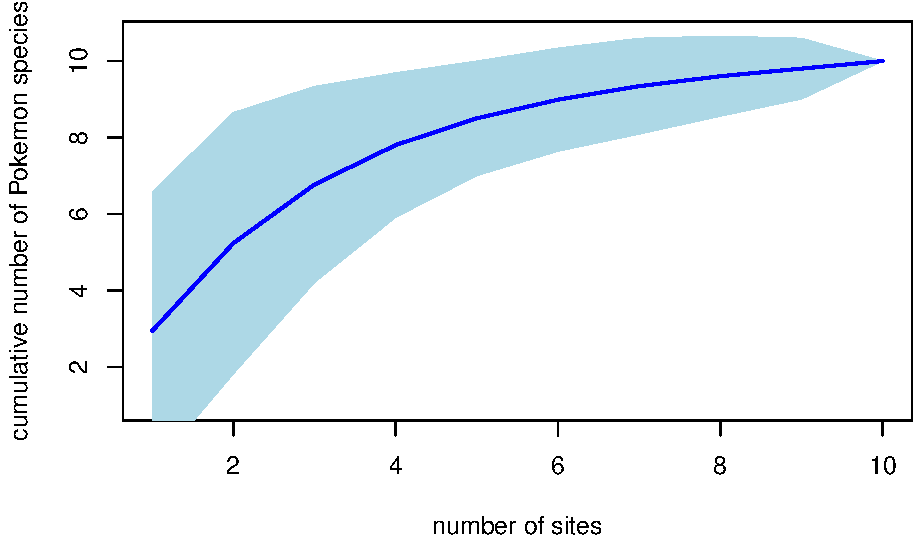
\includegraphics{macro-module_files/figure-latex/unnamed-chunk-27-1.pdf}

\texttt{"ci.type\ =\ "poly"} tells R that you want a shaded area showing
the confidence intervals from your randomisations. You can play around
with the colours etc. if you want to.

To demonstrate why we need the randomisations, look at two curves for
just 1 permutation each.

\begin{Shaded}
\begin{Highlighting}[]
\NormalTok{pokemon.curve1 <-}\StringTok{ }\KeywordTok{specaccum}\NormalTok{(pokemon.matrix, }\DataTypeTok{method =} \StringTok{"random"}\NormalTok{, }\DataTypeTok{permutations =} \DecValTok{1}\NormalTok{)}
\NormalTok{pokemon.curve2 <-}\StringTok{ }\KeywordTok{specaccum}\NormalTok{(pokemon.matrix, }\DataTypeTok{method =} \StringTok{"random"}\NormalTok{, }\DataTypeTok{permutations =} \DecValTok{1}\NormalTok{)}

\KeywordTok{par}\NormalTok{(}\DataTypeTok{mfrow =} \KeywordTok{c}\NormalTok{(}\DecValTok{1}\NormalTok{,}\DecValTok{2}\NormalTok{))}

\KeywordTok{plot}\NormalTok{(pokemon.curve1,  }
    \DataTypeTok{xlab =} \StringTok{"number of sites"}\NormalTok{, }\DataTypeTok{ylab =} \StringTok{"cumulative number of Pokemon species"}\NormalTok{)}

\KeywordTok{plot}\NormalTok{(pokemon.curve2, }
    \DataTypeTok{xlab =} \StringTok{"number of sites"}\NormalTok{, }\DataTypeTok{ylab =} \StringTok{"cumulative number of Pokemon species"}\NormalTok{)}
\end{Highlighting}
\end{Shaded}

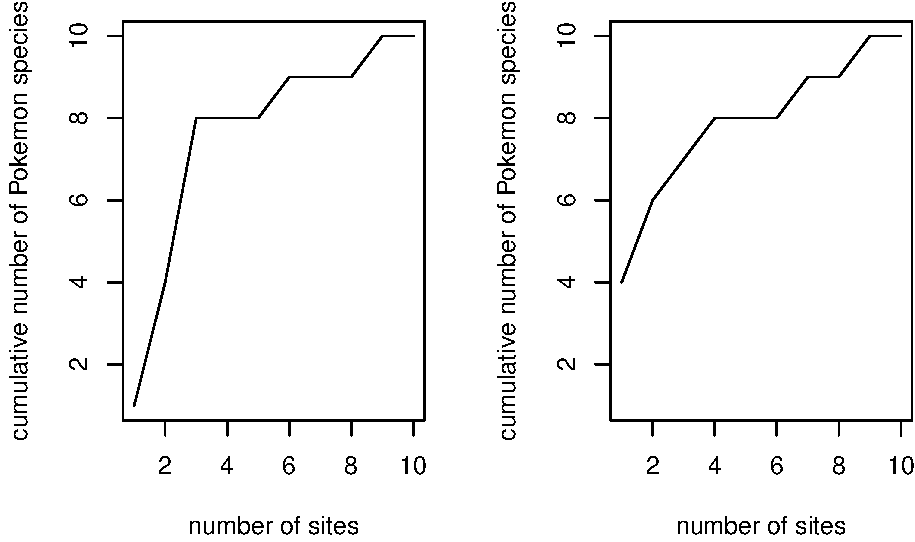
\includegraphics{macro-module_files/figure-latex/unnamed-chunk-28-1.pdf}

\begin{Shaded}
\begin{Highlighting}[]
\KeywordTok{par}\NormalTok{(}\DataTypeTok{mfrow =} \KeywordTok{c}\NormalTok{(}\DecValTok{1}\NormalTok{,}\DecValTok{1}\NormalTok{))}
\end{Highlighting}
\end{Shaded}

Finally to estimate total species richness across all sites we can
(again) use many different metrics. Some common ones include Chao 2
(Chao 1987), Jackknife and Bootstrapping approaches and these are easy
to estimate using the \texttt{vegan} function \texttt{specpool}.

\begin{Shaded}
\begin{Highlighting}[]
\KeywordTok{specpool}\NormalTok{(pokemon.matrix)}
\end{Highlighting}
\end{Shaded}

\begin{verbatim}
##     Species chao  chao.se jack1 jack1.se    jack2     boot   boot.se  n
## All      10 11.8 3.394113  11.8 1.272792 12.68889 10.90352 0.7502033 10
\end{verbatim}

Estimates range from 10.9 \(\pm\) 0.75 (bootstrap) to 11.8 \(\pm\) 3.39
(Chao2). So we can be fairly confident there are between 10 and 15
Pokemon in the Museum.

\begin{center}\rule{0.5\linewidth}{\linethickness}\end{center}

\section{References}\label{references}

\begin{itemize}
\tightlist
\item
  Chao, A. (1987). Estimating the population size for capture-recapture
  data with unequal catchability. Biometrics 43, 783--791.
\item
  Colwell, R.K. \& Coddington, J.A. (1994). Estimating terrestrial
  biodiversity through extrapolation. Phil. Trans. Roy. Soc. London B
  345, 101--118.
\item
  Hill, M. O. (1973) Diversity and evenness: a unifying notation and its
  consequences. Ecology, 54, 427--432
\item
  Koleff, P., Gaston, K.J. and Lennon, J.J. (2003) Measuring beta
  diversity for presence-absence data. Journal of Animal Ecology 72,
  367--382.
\item
  Whittaker, R.H. (1960) Vegetation of Siskiyou mountains, Oregon and
  California. Ecological Monographs 30, 279--338.
\item
  Whittaker, R. H. (1972). Evolution and Measurement of Species
  Diversity. Taxon, 21, 213-251. \url{doi:10.2307/1218190}
\end{itemize}

\subsection{Extra reading}\label{extra-reading}

\begin{itemize}
\tightlist
\item
  Whittaker, R. J. et al. (2001). Scale and species richness: towards a
  general, hierarchical theory of species diversity. Journal of
  Biogeography, 28, 453-470. \url{doi:10.1046/j.1365-2699.2001.00563.x}
\item
  O'Hara, R.B. (2005). Species richness estimators: how many species can
  dance on the head of a pin? J. Anim. Ecol. 74, 375--386.
\end{itemize}

\subsubsection{Nice series of papers on
betadiversity}\label{nice-series-of-papers-on-betadiversity}

\begin{itemize}
\tightlist
\item
  Tuomisto, H. (2010) A diversity of beta diversities: straightening up
  a concept gone awry. Part 1. Defining beta diversity as a function of
  alpha and gamma diversity. Ecography, 33, 2-22.
\item
  Tuomisto, H. (2010) A diversity of beta diversities: straightening up
  a concept gone awry. Part 2. Quantifying beta diversity and related
  phenomena. Ecography, 33, 23-45.
  \url{doi:10.1111/j.1600-0587.2009.06148.x}
\item
  Tuomisto, H. 2010. A consistent terminology for quantifying species
  diversity? Yes, it does exist. Oecologia 4: 853--860.
  \url{doi:10.1007/s00442-010-1812-0}
\item
  Tuomisto, H. (2011) Commentary: do we have a consistent terminology
  for species diversity? Yes, if we choose to use it. Oecologia, 167,
  903-911.
\end{itemize}

\subsubsection{Immensely cool new approach using methods developed by
Alan
Turing}\label{immensely-cool-new-approach-using-methods-developed-by-alan-turing}

\begin{itemize}
\tightlist
\item
  Chiu, C.H., Wang, Y.T., Walther, B.A. \& Chao, A. (2014). Improved
  nonparametric lower bound of species richness via a modified
  Good-Turing frequency formula. Biometrics 70, 671--682.
\end{itemize}

\chapter{Visualising phylogenies in
R}\label{visualising-phylogenies-in-r}

The aims of this practical are to introduce you to some of the fun ways
you can visualise phylogenetic trees in R. The code and examples are
based on Liam Revell's book chapter
\href{http://faculty.umb.edu/liam.revell/pdfs/Revell_2014.MPCM-chapter.pdf}{here}.

Note that some of these plots won't work very well in RStudio. You may
need to click the zoom button to see them, or resort to using the old R
GUI instead.

\textbf{REMEMBER}

\begin{itemize}
\tightlist
\item
  Download all of the data for the practical into a folder somewhere on
  your computer.
\item
  Set your working directory to this folder.
\item
  Start a new script for this practical.
\end{itemize}

You will also need to install the following packages:

\begin{itemize}
\tightlist
\item
  \texttt{ape}
\item
  \texttt{phytools}
\end{itemize}

\begin{center}\rule{0.5\linewidth}{\linethickness}\end{center}

First load the packages we need and the data.

\begin{Shaded}
\begin{Highlighting}[]
\KeywordTok{library}\NormalTok{(ape)}
\KeywordTok{library}\NormalTok{(phytools)}
\end{Highlighting}
\end{Shaded}

Later we will use some Greater Antillean \emph{Anolis} lizard data to
add data to a phylogeny. Before we can add data to our tree, we need to
load the data.

\begin{Shaded}
\begin{Highlighting}[]
\NormalTok{anoledata <-}\StringTok{ }\KeywordTok{read.csv}\NormalTok{(}\StringTok{"anole.data.csv"}\NormalTok{, }\DataTypeTok{header =} \OtherTok{TRUE}\NormalTok{)}

\CommentTok{# Look at the data}
\KeywordTok{str}\NormalTok{(anoledata)}
\end{Highlighting}
\end{Shaded}

\begin{verbatim}
## 'data.frame':    100 obs. of  23 variables:
##  $ species               : Factor w/ 100 levels "ahli","alayoni",..: 1 2 3 4 5 6 7 8 9 10 ...
##  $ AVG.SVL               : num  4.04 3.82 3.53 4.04 4.38 ...
##  $ AVG.hl                : num  2.88 2.7 2.38 2.9 3.36 ...
##  $ AVG.hw                : num  2.36 1.99 1.56 2.37 2.69 ...
##  $ AVG.hh                : num  2.13 1.75 1.39 2.05 2.32 ...
##  $ AVG.ljl               : num  2.85 2.71 2.32 2.9 3.38 ...
##  $ AVG.outlever          : num  2.75 2.62 2.26 2.83 3.29 ...
##  $ AVG.jugal.to.symphysis: num  2.54 2.37 2.08 2.6 3.07 ...
##  $ AVG.femur             : num  2.74 2.07 2.17 2.48 2.8 ...
##  $ AVG.tibia             : num  2.69 2.02 2.09 2.34 2.69 ...
##  $ AVG.met               : num  2.25 1.54 1.55 1.87 2.18 ...
##  $ AVG.ltoe.IV           : num  2.55 1.88 1.73 2.26 2.53 ...
##  $ AVG.toe.IV.lam.width  : num  0.1795 0.0488 -0.5361 0.4904 0.8441 ...
##  $ AVG.humerus           : num  2.46 1.95 1.63 2.3 2.62 ...
##  $ AVG.radius            : num  2.27 1.69 1.4 2.09 2.34 ...
##  $ AVG.lfing.IV          : num  1.94 1.4 1.04 1.7 1.98 ...
##  $ AVG.fing.IV.lam.width : num  0.0754 -0.0739 -0.755 0.3155 0.6584 ...
##  $ AVG.pelv.ht           : num  1.99 1.51 1.19 1.87 2.1 ...
##  $ AVG.pelv.wd           : num  1.71 1.419 0.946 1.752 2.014 ...
##  $ Foot.Lam.num          : num  3.28 3.43 3.2 3.58 3.72 ...
##  $ Hand.Lam.num          : num  2.87 3.08 2.73 3.16 3.24 ...
##  $ Avg.lnSVL2            : num  3.94 3.74 3.48 3.93 4.36 ...
##  $ Avg.ln.t1             : num  4.41 4 4.37 4.44 5.04 ...
\end{verbatim}

Now let's visualise some phylogenies!

\section{Loading your phylogeny and data into
R}\label{loading-your-phylogeny-and-data-into-r}

\subsection{Reading in a phylogeny from a
file}\label{reading-in-a-phylogeny-from-a-file}

To load a tree you need either the function \texttt{read.tree} or
\texttt{read.nexus}. \texttt{read.tree} can deal with a number of
different types of data (including DNA) whereas \texttt{read.nexus}
reads NEXUS files. \texttt{elopomorph.tre} is not in NEXUS format so we
use \texttt{read.tree}.

\begin{Shaded}
\begin{Highlighting}[]
\NormalTok{fishtree <-}\StringTok{ }\KeywordTok{read.tree}\NormalTok{(}\StringTok{"elopomorph.tre"}\NormalTok{)}
\end{Highlighting}
\end{Shaded}

\subsection{Reading in a phylogeny that is already built into
R}\label{reading-in-a-phylogeny-that-is-already-built-into-r}

The bird and anole phylogenies are already built into R so we don't need
to read them in using \texttt{read.tree}. Instead we just use:

\begin{Shaded}
\begin{Highlighting}[]
\KeywordTok{data}\NormalTok{(bird.orders)}
\KeywordTok{data}\NormalTok{(anoletree)}
\end{Highlighting}
\end{Shaded}

\section{Basic tree viewing in R}\label{basic-tree-viewing-in-r}

We'll use the Elopomorpha (eels and similar fishes) tree to start as it
is simple.

Let's examine the tree by typing:

\begin{Shaded}
\begin{Highlighting}[]
\NormalTok{fishtree}
\end{Highlighting}
\end{Shaded}

\begin{verbatim}
## 
## Phylogenetic tree with 62 tips and 61 internal nodes.
## 
## Tip labels:
##  Moringua_edwardsi, Kaupichthys_nuchalis, Gorgasia_taiwanensis, Heteroconger_hassi, Venefica_proboscidea, Anguilla_rostrata, ...
## 
## Rooted; includes branch lengths.
\end{verbatim}

\begin{Shaded}
\begin{Highlighting}[]
\KeywordTok{str}\NormalTok{(fishtree)}
\end{Highlighting}
\end{Shaded}

\begin{verbatim}
## List of 4
##  $ edge       : int [1:122, 1:2] 63 64 64 65 66 67 68 68 69 70 ...
##  $ Nnode      : int 61
##  $ tip.label  : chr [1:62] "Moringua_edwardsi" "Kaupichthys_nuchalis" "Gorgasia_taiwanensis" "Heteroconger_hassi" ...
##  $ edge.length: num [1:122] 0.0105 0.0672 0.00537 0.00789 0.00157 ...
##  - attr(*, "class")= chr "phylo"
##  - attr(*, "order")= chr "cladewise"
\end{verbatim}

\texttt{fishtree} is a fully resolved tree with branch lengths. There
are 62 species and 61 internal nodes. We can plot the tree by using the
\texttt{plot.phylo} function of \texttt{ape}. Note that we can just use
the function \texttt{plot} to do this as R knows if we ask it to plot a
phylogeny to use \texttt{plot.phylo} instead!

\begin{Shaded}
\begin{Highlighting}[]
\KeywordTok{plot}\NormalTok{(fishtree, }\DataTypeTok{cex =} \FloatTok{0.5}\NormalTok{)}
\end{Highlighting}
\end{Shaded}

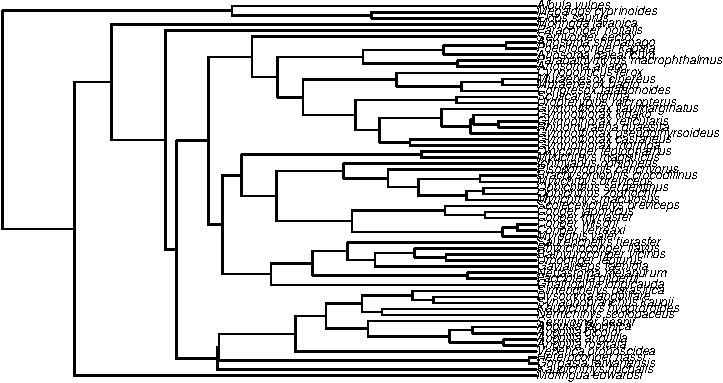
\includegraphics{macro-module_files/figure-latex/unnamed-chunk-35-1.pdf}

\texttt{cex\ =\ 0.5} reduces the size of the tip labels so we can read
them. We can also zoom into different sections of the tree that you're
interested in:

\begin{Shaded}
\begin{Highlighting}[]
\KeywordTok{zoom}\NormalTok{(fishtree, }\KeywordTok{grep}\NormalTok{(}\StringTok{"Gymnothorax"}\NormalTok{, fishtree$tip.label), }\DataTypeTok{subtree =} \OtherTok{FALSE}\NormalTok{, }\DataTypeTok{cex =} \FloatTok{0.8}\NormalTok{)}
\end{Highlighting}
\end{Shaded}

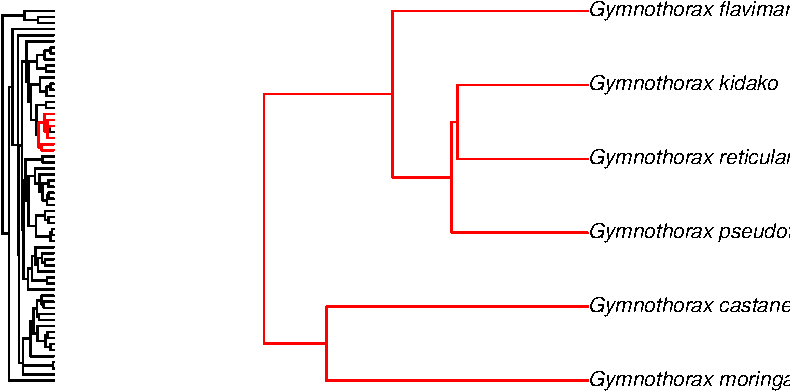
\includegraphics{macro-module_files/figure-latex/unnamed-chunk-36-1.pdf}

This just gives you the tree for \emph{Micropterus} species but you can
also see how the species fit into the rest of the tree using:

\begin{Shaded}
\begin{Highlighting}[]
\KeywordTok{zoom}\NormalTok{(fishtree, }\KeywordTok{grep}\NormalTok{(}\StringTok{"Gymnothorax"}\NormalTok{, fishtree$tip.label), }\DataTypeTok{subtree =} \OtherTok{TRUE}\NormalTok{, }\DataTypeTok{cex =} \FloatTok{0.8}\NormalTok{)}
\end{Highlighting}
\end{Shaded}

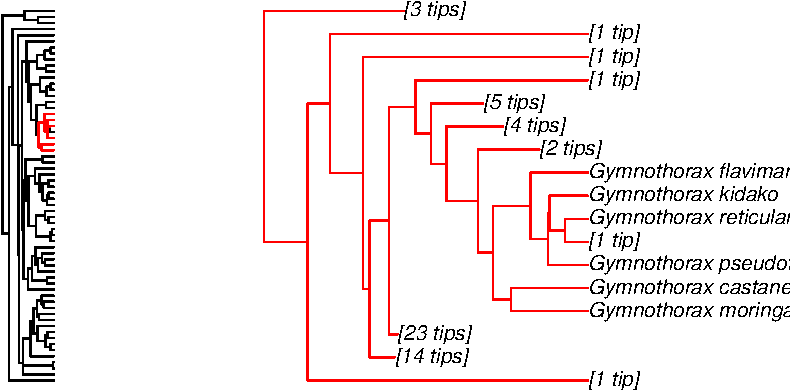
\includegraphics{macro-module_files/figure-latex/unnamed-chunk-37-1.pdf}

Note that \texttt{zoom} automatically sets the plotting window to
display two plots at once. To reset this to one plot only use:

\begin{Shaded}
\begin{Highlighting}[]
\KeywordTok{par}\NormalTok{(}\DataTypeTok{mfrow =} \KeywordTok{c}\NormalTok{(}\DecValTok{1}\NormalTok{, }\DecValTok{1}\NormalTok{))}
\end{Highlighting}
\end{Shaded}

To get further options for the plotting of phylogenies:

\begin{Shaded}
\begin{Highlighting}[]
\NormalTok{?plot.phylo}
\end{Highlighting}
\end{Shaded}

Note that although you can use \texttt{plot} to plot the phylogeny, you
need to specify \texttt{plot.phylo} to find out the options for plotting
trees. You can change the style of the tree (\texttt{type}), the color
of the branches and tips (\texttt{edge.color}, \texttt{tip.color}), and
the size of the tip labels (\texttt{cex}). Here's an fun/hideous
example!

\begin{Shaded}
\begin{Highlighting}[]
\KeywordTok{plot}\NormalTok{(fishtree, }\DataTypeTok{type =} \StringTok{"fan"}\NormalTok{, }\DataTypeTok{edge.color =} \StringTok{"deeppink"}\NormalTok{, }\DataTypeTok{tip.color =} \StringTok{"springgreen"}\NormalTok{, }
     \DataTypeTok{cex =} \FloatTok{0.5}\NormalTok{)}
\end{Highlighting}
\end{Shaded}

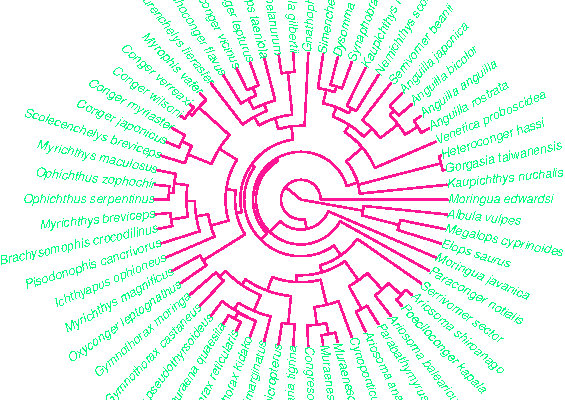
\includegraphics{macro-module_files/figure-latex/unnamed-chunk-40-1.pdf}

Or try

\begin{Shaded}
\begin{Highlighting}[]
\KeywordTok{plot}\NormalTok{(fishtree, }\DataTypeTok{type =} \StringTok{"c"}\NormalTok{, }\DataTypeTok{edge.color =} \StringTok{"darkviolet"}\NormalTok{, }\DataTypeTok{tip.color =} \StringTok{"hotpink"}\NormalTok{, }
     \DataTypeTok{cex =} \FloatTok{0.5}\NormalTok{)}
\end{Highlighting}
\end{Shaded}

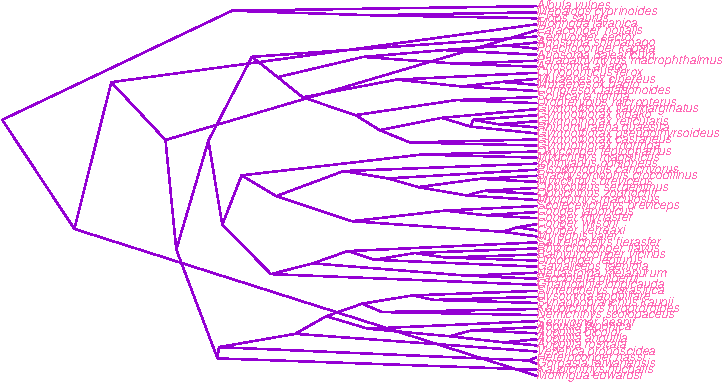
\includegraphics{macro-module_files/figure-latex/unnamed-chunk-41-1.pdf}

\section{Adding trait data to trees in
R}\label{adding-trait-data-to-trees-in-r}

\emph{Note that the theory behind this is covered in more detail in the
``Macroevolutionary Models in R'' practicals part 1 and 2.} \#\#\#
Ancestral state reconstructions on discrete data We will use the bird
data. Remember we already loaded the phylogeny and data as follows:

\begin{Shaded}
\begin{Highlighting}[]
\KeywordTok{data}\NormalTok{(bird.orders)}
\end{Highlighting}
\end{Shaded}

First we will invent some data for each bird order that we can
reconstruct along the tree. This creates three variables, 0, 1 and 2.

\begin{Shaded}
\begin{Highlighting}[]
\NormalTok{mydata <-}\StringTok{ }\KeywordTok{factor}\NormalTok{(}\KeywordTok{c}\NormalTok{(}\KeywordTok{rep}\NormalTok{(}\DecValTok{0}\NormalTok{, }\DecValTok{5}\NormalTok{), }\KeywordTok{rep}\NormalTok{(}\DecValTok{1}\NormalTok{, }\DecValTok{13}\NormalTok{), }\KeywordTok{rep}\NormalTok{(}\DecValTok{2}\NormalTok{, }\DecValTok{5}\NormalTok{)))}
\NormalTok{mydata}
\end{Highlighting}
\end{Shaded}

\begin{verbatim}
##  [1] 0 0 0 0 0 1 1 1 1 1 1 1 1 1 1 1 1 1 2 2 2 2 2
## Levels: 0 1 2
\end{verbatim}

We can then use the \texttt{ape} function \texttt{ace} to reconstruct
ancestral characters along the nodes of the tree. \texttt{type\ =\ d}
means the character to be reconstructed is discrete.

\begin{Shaded}
\begin{Highlighting}[]
\NormalTok{ancestors <-}\StringTok{ }\KeywordTok{ace}\NormalTok{(mydata, bird.orders, }\DataTypeTok{type =} \StringTok{"d"}\NormalTok{)}
\end{Highlighting}
\end{Shaded}

Now we can plot this on a phylogeny. First decide which colours we'd
like. To look at a list of colours in R type in \texttt{colors()}.

\begin{Shaded}
\begin{Highlighting}[]
\NormalTok{colours <-}\StringTok{ }\KeywordTok{c}\NormalTok{(}\StringTok{"cornflowerblue"}\NormalTok{, }\StringTok{"cyan4"}\NormalTok{, }\StringTok{"goldenrod"}\NormalTok{)}
\end{Highlighting}
\end{Shaded}

Now plot the tree and add labels to the tips and the nodes using the
results in \texttt{ancestors}. We use \texttt{label.offset\ =\ 1} to
move the labels to the right a bit so the pie charts will fit\ldots{}

\begin{Shaded}
\begin{Highlighting}[]
\KeywordTok{plot}\NormalTok{(bird.orders, }\DataTypeTok{label.offset =} \DecValTok{1}\NormalTok{)}
\KeywordTok{tiplabels}\NormalTok{(}\DataTypeTok{pch =} \DecValTok{21}\NormalTok{, }\DataTypeTok{bg =} \NormalTok{colours[}\KeywordTok{as.numeric}\NormalTok{(mydata)], }\DataTypeTok{cex =} \DecValTok{2}\NormalTok{, }\DataTypeTok{adj =} \DecValTok{1}\NormalTok{)}
\KeywordTok{nodelabels}\NormalTok{(}\DataTypeTok{pie =} \NormalTok{ancestors$lik.anc, }\DataTypeTok{piecol =} \NormalTok{colours)}
\end{Highlighting}
\end{Shaded}

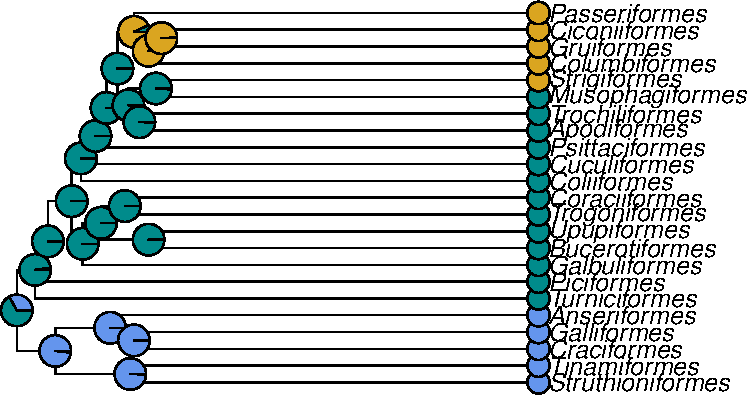
\includegraphics{macro-module_files/figure-latex/unnamed-chunk-46-1.pdf}

\texttt{pch\ =\ 21} sets the tip labels to be unfilled circles,
\texttt{bg} defines the colours of the circles using the list of colours
we provided, and ordering them based on what the species value was for
mydata (i.e.~0, 1 or 2). \texttt{cex\ =\ 2} doubles the point size, and
\texttt{adj\ =\ 1} moves the tip labels sideways so they don't obscure
the ends of the branches. \texttt{pie} makes pie charts coloured using
the ancestral state reconstructions in \texttt{ancestors}, and
\texttt{piecol} tells it to use the colours we have defined.

\subsection{Ancestral state reconstructions on continuous
data}\label{ancestral-state-reconstructions-on-continuous-data}

We are going to use the \emph{Anolis} data to create a phylogeny with
different colours for different observed and reconstructed body sizes
(snout-to-vent length, SVL). Remember we already loaded the phylogeny
and data as follows:

\begin{Shaded}
\begin{Highlighting}[]
\KeywordTok{data}\NormalTok{(anoletree)}
\NormalTok{anoledata <-}\StringTok{ }\KeywordTok{read.csv}\NormalTok{(}\StringTok{"anole.data.csv"}\NormalTok{, }\DataTypeTok{header =} \OtherTok{TRUE}\NormalTok{, }\DataTypeTok{row.names =} \DecValTok{1}\NormalTok{) }
\end{Highlighting}
\end{Shaded}

Note the names in \texttt{anoledata} are the species names without the
Genus. In the phylogeny the species names are \texttt{Anolis\_species}.
So to get the two to match we need to add \texttt{Anolis\_} to each
name.

\begin{Shaded}
\begin{Highlighting}[]
\KeywordTok{rownames}\NormalTok{(anoledata) <-}\StringTok{ }\KeywordTok{paste}\NormalTok{(}\StringTok{"Anolis"}\NormalTok{, }\KeywordTok{rownames}\NormalTok{(anoledata), }\DataTypeTok{sep =} \StringTok{"_"}\NormalTok{)}
\end{Highlighting}
\end{Shaded}

\texttt{paste} just sticks together \texttt{Anolis} with the names in
\texttt{anoles} already with an underscore (\texttt{\_}) separating them
(\texttt{sep\ =\ "\_"})

We then need to make sure the order of the species in the data matches
that of the phylogeny.

\begin{Shaded}
\begin{Highlighting}[]
\NormalTok{anoledata <-}\StringTok{ }\NormalTok{anoledata[anoletree$tip.label, ]}
\end{Highlighting}
\end{Shaded}

Next we make a matrix containing only the SVL values for each
\emph{Anolis} species:

\begin{Shaded}
\begin{Highlighting}[]
\NormalTok{SVL <-}\StringTok{ }\KeywordTok{as.matrix}\NormalTok{(anoledata)[,}\StringTok{"AVG.SVL"}\NormalTok{]}
\end{Highlighting}
\end{Shaded}

This code selects only the variable \texttt{AVG.SVL} from
\texttt{anoledata} (square brackets subset in R in the form {[}rows,
columns{]}), and then uses \texttt{as.matrix} to make this into a
matrix.

Take a look at \texttt{SVL}

\begin{Shaded}
\begin{Highlighting}[]
\KeywordTok{head}\NormalTok{(SVL)}
\end{Highlighting}
\end{Shaded}

\begin{verbatim}
##        Anolis_ahli     Anolis_allogus Anolis_rubribarbus 
##           4.039125           4.040138           4.078469 
##       Anolis_imias      Anolis_sagrei     Anolis_bremeri 
##           4.099687           4.067162           4.113371
\end{verbatim}

We then use the function \texttt{contMap}. \texttt{contMap} creates a
tree with a mapped continuous character, i.e.~where the value of the
character is known at the tips, and estimated along the tree. The
estimating of the character along the tree uses a Maximum Likelihood
estimation procedure. Here we will tell \texttt{contMap} not to
automatically plot the tree (using \texttt{plot\ =\ FALSE}) so we can
make some modifications.

\begin{Shaded}
\begin{Highlighting}[]
\NormalTok{SVLplot <-}\StringTok{ }\KeywordTok{contMap}\NormalTok{(anoletree, SVL, }\DataTypeTok{plot =} \OtherTok{FALSE}\NormalTok{)}
\end{Highlighting}
\end{Shaded}

For some reason this code breaks\ldots{}

Finally let's plot the tree as a fan (\texttt{legend\ =\ 10} just
spreads the legend out so it is readable).

\begin{Shaded}
\begin{Highlighting}[]
\KeywordTok{plot}\NormalTok{(SVLplot, }\DataTypeTok{type =} \StringTok{"fan"}\NormalTok{, }\DataTypeTok{legend =} \DecValTok{10}\NormalTok{)}
\end{Highlighting}
\end{Shaded}

\begin{verbatim}
## legend scale cannot be longer than total tree length; resetting
\end{verbatim}

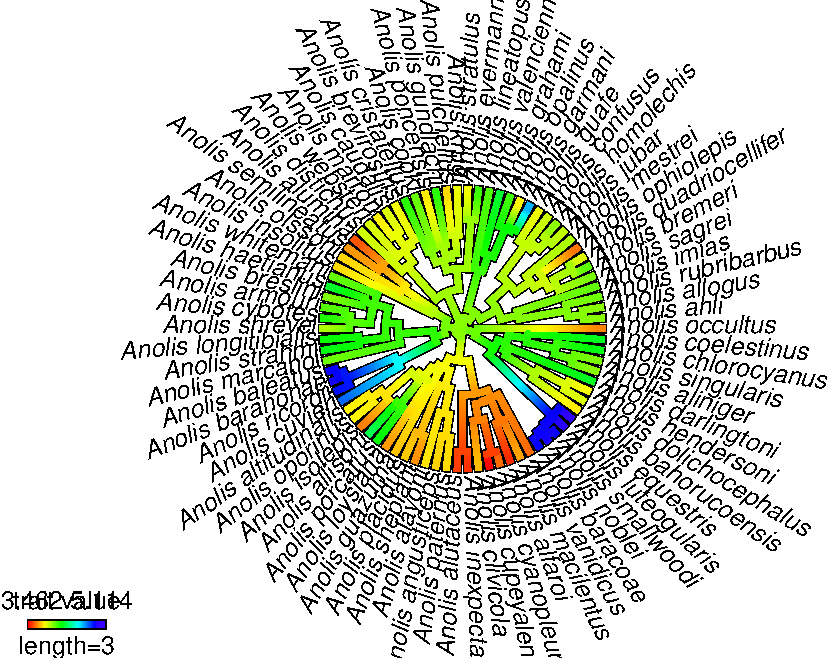
\includegraphics{macro-module_files/figure-latex/unnamed-chunk-53-1.pdf}

\section{Phylomorphospace plots in R}\label{phylomorphospace-plots-in-r}

We are going to use the \emph{Anolis} data to create a phylomorphospace
plot. These plots show where species fall within a morphospace (usually
based on principal components analyses of morphological variables), and
then reconstructs values for the nodes of the phylogeny so the whole
phylogeny can be projected into the morphospace.

We already loaded the phylogeny and data as follows:

\begin{Shaded}
\begin{Highlighting}[]
\KeywordTok{data}\NormalTok{(anoletree)}
\NormalTok{anoledata <-}\StringTok{ }\KeywordTok{read.csv}\NormalTok{(}\StringTok{"anole.data.csv"}\NormalTok{, }\DataTypeTok{header =} \OtherTok{TRUE}\NormalTok{, }\DataTypeTok{row.names =} \DecValTok{1}\NormalTok{)}
\end{Highlighting}
\end{Shaded}

As we saw above, the names of \texttt{anoles} are the species names
without the Genus. In the phylogeny the species names are
\texttt{Anolis\_species}. So to get the two to match we need to add
\texttt{Anolis\_} to each name.

\begin{Shaded}
\begin{Highlighting}[]
\KeywordTok{rownames}\NormalTok{(anoledata) <-}\StringTok{ }\KeywordTok{paste}\NormalTok{(}\StringTok{"Anolis"}\NormalTok{, }\KeywordTok{rownames}\NormalTok{(anoledata), }\DataTypeTok{sep =} \StringTok{"_"}\NormalTok{)}
\end{Highlighting}
\end{Shaded}

\texttt{paste} just sticks together \texttt{Anolis} with the names in
\texttt{anoles} already with an underscore (\texttt{\_}) separating them
(\texttt{sep\ =\ "\_"})

Next we again need to make sure the order of the species in the data
matches that of the phylogeny.

\begin{Shaded}
\begin{Highlighting}[]
\NormalTok{anoledata <-}\StringTok{ }\NormalTok{anoledata[anoletree$tip.label, ]}
\end{Highlighting}
\end{Shaded}

We can now run a phylogenetic principal components analysis on our
morphological trait data and extract the PC scores for each PC axis
using \texttt{\$S}.

\begin{Shaded}
\begin{Highlighting}[]
\NormalTok{PC <-}\StringTok{ }\KeywordTok{phyl.pca}\NormalTok{(anoletree, anoledata)$S}
\end{Highlighting}
\end{Shaded}

To plot the morphospace with colours, we need to define them. Here we
choose six colours, and matched them with the ecomorph types listed
\href{https://en.wikipedia.org/wiki/Anolis_ecomorphs}{here}. These were
built into \texttt{anoletree}.

\begin{Shaded}
\begin{Highlighting}[]
\NormalTok{colors <-}\StringTok{ }\KeywordTok{setNames}\NormalTok{(}\KeywordTok{c}\NormalTok{(}\StringTok{"cornflowerblue"}\NormalTok{, }\StringTok{"goldenrod"}\NormalTok{, }\StringTok{"chartreuse"}\NormalTok{, }\StringTok{"hotpink"}\NormalTok{,}
                     \StringTok{"orangered"}\NormalTok{, }\StringTok{"darkviolet"}\NormalTok{), }
                     \KeywordTok{sort}\NormalTok{(}\KeywordTok{unique}\NormalTok{(}\KeywordTok{getStates}\NormalTok{(anoletree, }\StringTok{"tips"}\NormalTok{))))}
\end{Highlighting}
\end{Shaded}

Finally we can make the plot, and colour by ecomorph.
\texttt{label\ =\ "off"} suppresses the printing of tip labels which
keeps things a bit tidier.

\begin{Shaded}
\begin{Highlighting}[]
\KeywordTok{phylomorphospace}\NormalTok{(anoletree, PC[,}\DecValTok{1}\NormalTok{:}\DecValTok{2}\NormalTok{], }\DataTypeTok{label =} \StringTok{"off"}\NormalTok{, }\DataTypeTok{node.by.map =} \OtherTok{TRUE}\NormalTok{, }\DataTypeTok{colors =} \NormalTok{colors)}
\end{Highlighting}
\end{Shaded}

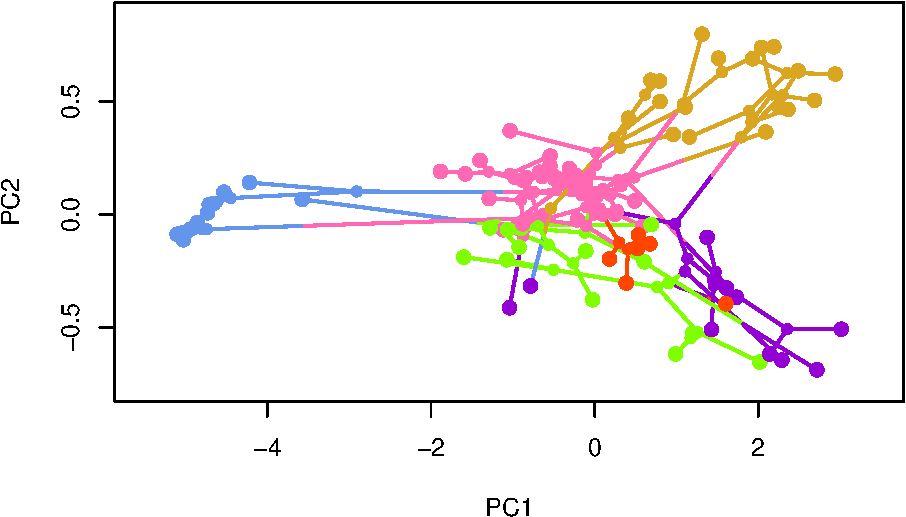
\includegraphics{macro-module_files/figure-latex/unnamed-chunk-59-1.pdf}

\section{Phylogenies and maps!}\label{phylogenies-and-maps}

We can also plot phylogenies attached to maps showing where species come
from. We will use the bird orders tree again as it's small.

\begin{Shaded}
\begin{Highlighting}[]
\KeywordTok{data}\NormalTok{(bird.orders)}
\end{Highlighting}
\end{Shaded}

We don't know where the birds come from, so we will simulate some
latitude and longitude data as follows. This uses a function that
simulates traits along the phylogeny, so close relatives should end up
with more similar latitude and longitude values. I've used high rates of
evolution (\texttt{sig2}) to force the points to be spread out. Of
course these values will be nonsensical for birds!

\begin{Shaded}
\begin{Highlighting}[]
\NormalTok{lat <-}\StringTok{ }\KeywordTok{fastBM}\NormalTok{(bird.orders, }\DataTypeTok{sig2 =} \DecValTok{100}\NormalTok{, }\DataTypeTok{bounds =} \KeywordTok{c}\NormalTok{(-}\DecValTok{90}\NormalTok{, }\DecValTok{90}\NormalTok{))}
\NormalTok{long <-}\StringTok{ }\KeywordTok{fastBM}\NormalTok{(bird.orders, }\DataTypeTok{sig2 =} \DecValTok{150}\NormalTok{, }\DataTypeTok{bounds =} \KeywordTok{c}\NormalTok{(-}\DecValTok{180}\NormalTok{, }\DecValTok{180}\NormalTok{))}
\end{Highlighting}
\end{Shaded}

Then we use the function \texttt{phylo.to.map} to match the locations
with the world map. This produces some output in the form
\texttt{objective\ 98} etc. (I have suppressed it here).

\begin{Shaded}
\begin{Highlighting}[]
\NormalTok{phylomap <-}\StringTok{ }\KeywordTok{phylo.to.map}\NormalTok{(bird.orders, }\KeywordTok{cbind}\NormalTok{(lat,long), }\DataTypeTok{plot =} \OtherTok{FALSE}\NormalTok{)}
\end{Highlighting}
\end{Shaded}

We can either put the phylogeny next to the map and draw lines to the
places they come from using \texttt{type\ =\ "phylogram"}\ldots{}

\begin{Shaded}
\begin{Highlighting}[]
\KeywordTok{plot}\NormalTok{(phylomap,}\DataTypeTok{type =} \StringTok{"phylogram"}\NormalTok{, }\DataTypeTok{asp =} \FloatTok{1.3}\NormalTok{, }\DataTypeTok{mar =} \KeywordTok{c}\NormalTok{(}\FloatTok{0.1}\NormalTok{, }\FloatTok{0.5}\NormalTok{, }\FloatTok{3.1}\NormalTok{, }\FloatTok{0.1}\NormalTok{))}
\end{Highlighting}
\end{Shaded}

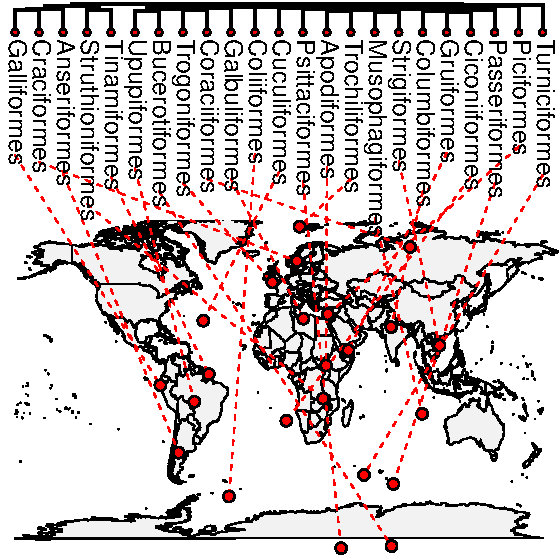
\includegraphics{macro-module_files/figure-latex/unnamed-chunk-63-1.pdf}

\ldots{}or plot the phylogeny directly onto the map using
\texttt{type\ =\ "direct"}

\begin{Shaded}
\begin{Highlighting}[]
\KeywordTok{plot}\NormalTok{(phylomap,}\DataTypeTok{type =} \StringTok{"direct"}\NormalTok{, }\DataTypeTok{asp =} \FloatTok{1.3}\NormalTok{, }\DataTypeTok{mar =} \KeywordTok{c}\NormalTok{(}\FloatTok{0.1}\NormalTok{, }\FloatTok{0.5}\NormalTok{, }\FloatTok{3.1}\NormalTok{, }\FloatTok{0.1}\NormalTok{))}
\end{Highlighting}
\end{Shaded}

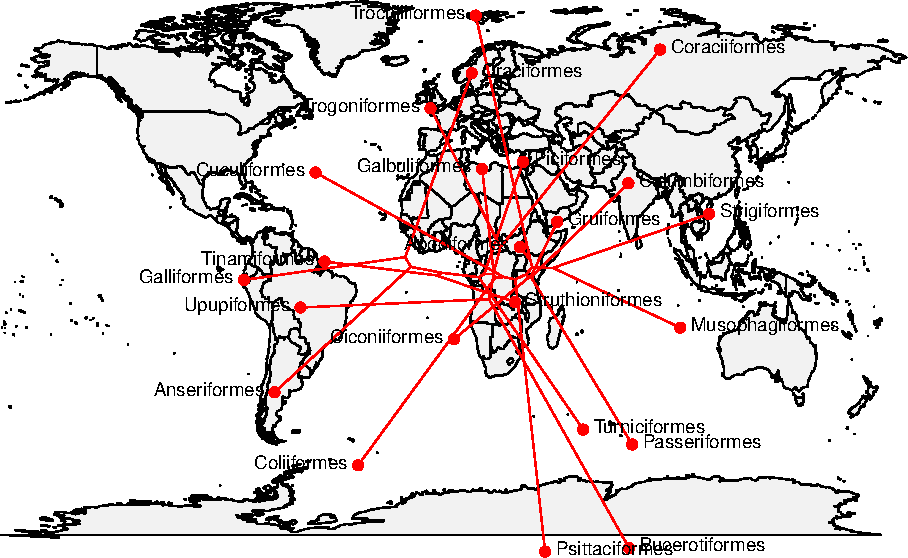
\includegraphics{macro-module_files/figure-latex/unnamed-chunk-64-1.pdf}

\section{A new package for visualising trees:
ggtree}\label{a-new-package-for-visualising-trees-ggtree}

\texttt{ggtree} is a newly released package that works with the popular
\texttt{ggplot} framework in R. \texttt{ggplot} works by adding layers
of different features together. A standard \texttt{ggplot} includes a
layer that assigns the x and y variables then can have lots of other
layers of points, lines, shapes and now with \texttt{ggtree}
phylogenies.

\textbf{Unfortunately this is broken in the most recent version of R.
I've left this in, just in case they fix it soon}

To use \texttt{ggtree} you will have to install it, then load it using:

\begin{Shaded}
\begin{Highlighting}[]
\KeywordTok{library}\NormalTok{(ggtree)}
\end{Highlighting}
\end{Shaded}

Let's replicate some of the stuff we did above but using
\texttt{ggtree}. As always choose whichever method you prefer when
you're doing this with your own data.

\begin{Shaded}
\begin{Highlighting}[]
\KeywordTok{ggtree}\NormalTok{(fishtree) +}
\KeywordTok{geom_text}\NormalTok{(}\KeywordTok{aes}\NormalTok{(}\DataTypeTok{label=}\NormalTok{label), }\DataTypeTok{size =} \DecValTok{1}\NormalTok{)}
\end{Highlighting}
\end{Shaded}

Note that the layers here are the tree, and then the tip labels. Layers
are separated by \texttt{+}

We can also zoom in on sections like with \texttt{ape}.

\begin{Shaded}
\begin{Highlighting}[]
\KeywordTok{gzoom}\NormalTok{(fishtree, }\KeywordTok{grep}\NormalTok{(}\StringTok{"Gymnothorax"}\NormalTok{, fishtree$tip.label))}
\end{Highlighting}
\end{Shaded}

And we can have different shapes of phylogeny, different colours and
even different line types.

\begin{Shaded}
\begin{Highlighting}[]
\KeywordTok{ggtree}\NormalTok{(fishtree, }\DataTypeTok{color =} \StringTok{"steelblue"}\NormalTok{)}
\KeywordTok{ggtree}\NormalTok{(fishtree, }\DataTypeTok{layout =} \StringTok{"circular"}\NormalTok{)}
\KeywordTok{ggtree}\NormalTok{(fishtree, }\DataTypeTok{linetype =} \StringTok{"dotted"}\NormalTok{)}
\end{Highlighting}
\end{Shaded}

\texttt{ggtree} is really great for highlighting sections of a tree.
First look at the nodes on your tree and pick an interesting one\ldots{}

\begin{Shaded}
\begin{Highlighting}[]
\KeywordTok{ggtree}\NormalTok{(fishtree) +}\StringTok{ }
\StringTok{  }\KeywordTok{geom_text}\NormalTok{(}\KeywordTok{aes}\NormalTok{(}\DataTypeTok{label =} \NormalTok{node))}
\end{Highlighting}
\end{Shaded}

Then highlight and/or annotate\ldots{}

\begin{Shaded}
\begin{Highlighting}[]
\KeywordTok{ggtree}\NormalTok{(fishtree) +}
\KeywordTok{geom_hilight}\NormalTok{(}\DataTypeTok{node =} \DecValTok{73}\NormalTok{, }\DataTypeTok{fill =} \StringTok{"steelblue"}\NormalTok{, }\DataTypeTok{alpha =} \FloatTok{0.6}\NormalTok{) +}
\KeywordTok{geom_hilight}\NormalTok{(}\DataTypeTok{node =} \DecValTok{97}\NormalTok{, }\DataTypeTok{fill =} \StringTok{"darkgreen"}\NormalTok{, }\DataTypeTok{alpha =} \FloatTok{0.6}\NormalTok{)}
\end{Highlighting}
\end{Shaded}

This package has a huge amount of promise, but still a few bugs and
weird features (it's designed by geneticists who are used to dealing
with short species labels, hence the issues getting our species names to
actually fit on the plot). The help files are also currently a bit
sparse and some of the vignette examples don't work. But if you're
likely to need to do any of this kind of stuff I recommend checking out
the vignette and the paper:

\begin{itemize}
\tightlist
\item
  Guangchuang Yu, David Smith, Huachen Zhu, Yi Guan, Tommy Tsan-Yuk Lam.
  ggtree: an R package for visualization and annotation of phylogenetic
  trees with their covariates and other associated data. \emph{Methods
  in Ecology and Evolution} 2016, \url{doi:10.1111/2041-210X.12628}.
\end{itemize}

\chapter{Phylogenetic Generalised Least Squares (PGLS) in
R}\label{phylogenetic-generalised-least-squares-pgls-in-r}

The aims of this practical are to learn how to use R to perform
Phylogenetic Generalised Least Squares (PGLS) analyses, and to estimate
phylogenetic signal.

We will be using the evolution of primate life-history variables as an
example. These data come from the PanTHERIA database (Jones et al. 2009)
and 10kTrees (Arnold et al. 2010). Note that this is an old version of
10kTrees, so if you want to use it in your research please download the
newest version.

\textbf{REMEMBER}

\begin{itemize}
\tightlist
\item
  Download all of the data for the practical into a folder somewhere on
  your computer.
\item
  Set your working directory to this folder.
\item
  Start a new script for this practical.
\end{itemize}

You will also need to install the following packages:

\begin{itemize}
\tightlist
\item
  \texttt{ape}
\item
  \texttt{geiger}
\item
  \texttt{picante}
\item
  \texttt{caper}
\end{itemize}

\begin{center}\rule{0.5\linewidth}{\linethickness}\end{center}

\section{Preparing for the analysis}\label{preparing-for-the-analysis}

\subsection{Load the required
packages}\label{load-the-required-packages}

To begin we need to load the packages for this practical.

\begin{Shaded}
\begin{Highlighting}[]
\KeywordTok{library}\NormalTok{(ape)}
\KeywordTok{library}\NormalTok{(geiger)}
\KeywordTok{library}\NormalTok{(picante)}
\KeywordTok{library}\NormalTok{(caper)}
\end{Highlighting}
\end{Shaded}

\subsection{Reading and checking your data in
R}\label{reading-and-checking-your-data-in-r}

The data are in a comma-delimited text file called
\texttt{Primatedata.csv}. Load these data as follows. I am assuming you
have set your working directory.

\begin{Shaded}
\begin{Highlighting}[]
\NormalTok{primatedata <-}\StringTok{ }\KeywordTok{read.csv}\NormalTok{(}\StringTok{"Primatedata.csv"}\NormalTok{)}
\end{Highlighting}
\end{Shaded}

Check everything loaded correctly:

\begin{Shaded}
\begin{Highlighting}[]
\KeywordTok{str}\NormalTok{(primatedata)}
\end{Highlighting}
\end{Shaded}

\begin{verbatim}
## 'data.frame':    77 obs. of  9 variables:
##  $ Order          : Factor w/ 1 level "Primates": 1 1 1 1 1 1 1 1 1 1 ...
##  $ Family         : Factor w/ 15 levels "Aotidae","Atelidae",..: 2 2 2 14 3 3 3 4 4 4 ...
##  $ Binomial       : Factor w/ 77 levels "Alouatta palliata",..: 5 6 7 8 9 10 11 15 16 17 ...
##  $ AdultBodyMass_g: num  6692 7582 8697 958 558 ...
##  $ GestationLen_d : num  138 226 228 164 154 ...
##  $ HomeRange_km2  : num  2.28 0.73 1.36 0.02 0.32 0.02 0.00212 0.51 0.16 0.24 ...
##  $ MaxLongevity_m : num  336 328 454 304 215 ...
##  $ SocialGroupSize: num  14.5 42 20 2.95 6.85 ...
##  $ SocialStatus   : int  2 2 2 2 2 2 2 2 2 2 ...
\end{verbatim}

As you can see, the data contains the following variables: Order,
Family, Binomial, AdultBodyMass\_g, GestationLen\_d, HomeRange\_km2,
MaxLongevity\_m, and SocialGroupSize.

\subsection{Reading and checking your phylogeny in
R}\label{reading-and-checking-your-phylogeny-in-r}

To load a tree you need either the function \texttt{read.tree} or
\texttt{read.nexus}. \texttt{read.tree} can deal with a number of
different types of data (including DNA) whereas \texttt{read.nexus}
reads NEXUS files. We will use a NEXUS file of the consensus tree from
10kTrees.

\begin{Shaded}
\begin{Highlighting}[]
\NormalTok{primatetree <-}\KeywordTok{read.nexus}\NormalTok{(}\StringTok{"consensusTree_10kTrees_Version2.nex"}\NormalTok{)}
\end{Highlighting}
\end{Shaded}

Let's examine the tree by typing:

\begin{Shaded}
\begin{Highlighting}[]
\NormalTok{primatetree}
\end{Highlighting}
\end{Shaded}

\begin{verbatim}
## 
## Phylogenetic tree with 226 tips and 221 internal nodes.
## 
## Tip labels:
##  Allenopithecus_nigroviridis, Cercopithecus_ascanius, Cercopithecus_cephus, Cercopithecus_cephus_cephus, Cercopithecus_cephus_ngottoensis, Cercopithecus_diana, ...
## 
## Rooted; includes branch lengths.
\end{verbatim}

\begin{Shaded}
\begin{Highlighting}[]
\KeywordTok{str}\NormalTok{(primatetree)}
\end{Highlighting}
\end{Shaded}

\begin{verbatim}
## List of 4
##  $ edge       : int [1:446, 1:2] 227 228 229 230 231 232 233 234 234 235 ...
##  $ edge.length: num [1:446] 4.95 17.69 19.65 8.12 4.82 ...
##  $ Nnode      : int 221
##  $ tip.label  : chr [1:226] "Allenopithecus_nigroviridis" "Cercopithecus_ascanius" "Cercopithecus_cephus" "Cercopithecus_cephus_cephus" ...
##  - attr(*, "class")= chr "phylo"
##  - attr(*, "order")= chr "cladewise"
\end{verbatim}

\begin{Shaded}
\begin{Highlighting}[]
\CommentTok{# It's usually a good idea to quickly plot the tree too}
\KeywordTok{plot}\NormalTok{(primatetree, }\DataTypeTok{cex =} \FloatTok{0.2}\NormalTok{, }\DataTypeTok{typ =} \StringTok{"fan"}\NormalTok{)}
\end{Highlighting}
\end{Shaded}

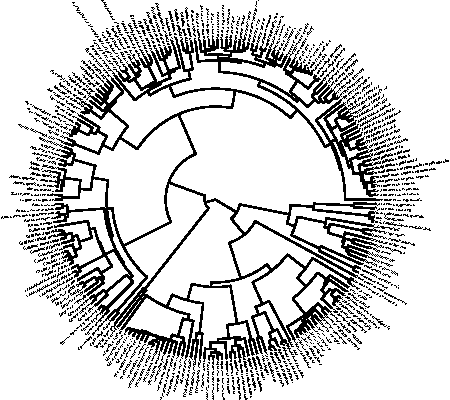
\includegraphics{macro-module_files/figure-latex/unnamed-chunk-75-1.pdf}

\texttt{primatetree} is a fully resolved tree with branch lengths. There
are 226 species and 221 internal nodes.

Most R functions require your tree to be dichotomous, i.e.~to have no
polytomies. To check whether your tree is dichotomous use
\texttt{is.binary.tree}. If this is FALSE, use \texttt{multi2di} to make
the tree dichotomous. This function works by randomly resolving
polytomies with zero-length branches.

\begin{Shaded}
\begin{Highlighting}[]
\KeywordTok{is.binary.tree}\NormalTok{(primatetree) }\CommentTok{# We want this to be TRUE}
\end{Highlighting}
\end{Shaded}

\begin{verbatim}
## [1] FALSE
\end{verbatim}

\begin{Shaded}
\begin{Highlighting}[]
\NormalTok{primatetree <-}\StringTok{ }\KeywordTok{multi2di}\NormalTok{(primatetree)}
\end{Highlighting}
\end{Shaded}

Most functions also require the tree to be rooted, i.e., to have one
taxon designated as the outgroup. Our tree is rooted but if you wanted
to change the root, or root an unrooted tree use \texttt{root}. Note
that here I've just chosen a random species \emph{Saimiri sciureus} to
be the root.

\begin{Shaded}
\begin{Highlighting}[]
\NormalTok{primatetree.reroot <-}\StringTok{ }\KeywordTok{root}\NormalTok{(primatetree, }\StringTok{"Saimiri_sciureus"}\NormalTok{)}
\KeywordTok{plot}\NormalTok{(primatetree.reroot, }\DataTypeTok{cex =} \FloatTok{0.2}\NormalTok{)}
\end{Highlighting}
\end{Shaded}

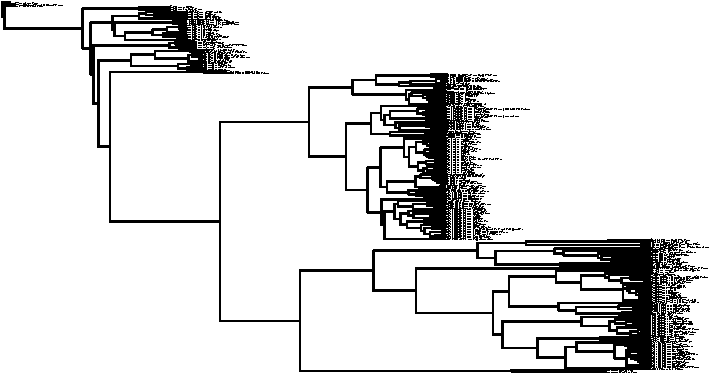
\includegraphics{macro-module_files/figure-latex/unnamed-chunk-78-1.pdf}

\subsection{Manipulating your data and phylogeny in
R}\label{manipulating-your-data-and-phylogeny-in-r}

\subsubsection{Species names with
spaces}\label{species-names-with-spaces}

Species names in the tree cannot contain spaces so they are generally
written as Genus\_species (the gap between the genus name and species
name replaced by an underscore \texttt{\_}). If the species names in the
data are written as Genus species with a space, then you will have to
replace the spaces with \texttt{\_} so that they match up with the
species names in the tree. You can do this as follows:

\begin{Shaded}
\begin{Highlighting}[]
\NormalTok{primatedata$Binomial <-}\StringTok{ }\KeywordTok{gsub}\NormalTok{(}\StringTok{" "}\NormalTok{, }\StringTok{"_"}\NormalTok{, primatedata$Binomial)}
\end{Highlighting}
\end{Shaded}

\texttt{gsub} means general substitution. It replaces any instance of
the first item (here it's a space) with the second item (\_) but only in
the variable you tell it to (\texttt{primatedata\$Binomial}).

\subsubsection{Mismatches between species in your data and
phylogeny}\label{mismatches-between-species-in-your-data-and-phylogeny}

Often you will have data for species which are not in your phylogeny
and/or species in your phylogeny which are not in your data. Some
functions in R can deal with this, others will produce an error telling
you the tree and data do not match (e.g.~most \texttt{ape} functions).
It's useful to know how to deal with this so I have provided code below.

Note that the \texttt{caper} function \texttt{comparative.data} (see
below) matches up species names in the tree and data for you before you
run any analyses. All \texttt{geiger} functions match the tree and the
data too. However, these functions are only as good as their inputs. If
you have even slightly misspelled a species name in the tree or the data
it will automatically be dropped from the analyses. It is therefore
\textbf{very important} to check this before running an analysis.

First we can use the function \texttt{name.check} to find out which
names do not match.

\begin{Shaded}
\begin{Highlighting}[]
\NormalTok{check <-}\StringTok{ }\KeywordTok{name.check}\NormalTok{(}\DataTypeTok{phy =} \NormalTok{primatetree, }\DataTypeTok{data =} \NormalTok{primatedata, }\DataTypeTok{data.names =} \NormalTok{primatedata$Binomial)}
\end{Highlighting}
\end{Shaded}

You can look at \texttt{check} by printing it, I won't do this here as
it produces a lot of output but take a look on your computer.

\begin{Shaded}
\begin{Highlighting}[]
\NormalTok{check}
\end{Highlighting}
\end{Shaded}

\texttt{check} has two parts, \texttt{tree\_not\_data} for species in
the tree but not in the dataset, and \texttt{data\_not\_tree} for
species in the dataset but not in the tree.

We can remove species missing from the tree easily using
\texttt{drop.tip} as we did above. You need to list the species which
you do \textbf{not} want to select and then drop them from the tree
instead of selecting the species you do want.

\begin{Shaded}
\begin{Highlighting}[]
\NormalTok{primatetree <-}\StringTok{ }\KeywordTok{drop.tip}\NormalTok{(primatetree, check$tree_not_data)}
\end{Highlighting}
\end{Shaded}

In this case we don't have any species in the tree missing from the
data, \texttt{data\_not\_tree} contains no species. However, if you do,
to remove species from the data which are not in the tree you can use
\texttt{match} and \texttt{subset} as follows:

\begin{Shaded}
\begin{Highlighting}[]
\NormalTok{matches <-}\StringTok{ }\KeywordTok{match}\NormalTok{(primatedata$Binomial, check$data_not_tree, }\DataTypeTok{nomatch =} \DecValTok{0}\NormalTok{)}
\NormalTok{primatedata <-}\StringTok{ }\KeywordTok{subset}\NormalTok{(primatedata, matches ==}\StringTok{ }\DecValTok{0}\NormalTok{)}
\end{Highlighting}
\end{Shaded}

\texttt{==} means \emph{equals}. So this line of code selects species
which do appear in the \texttt{data\_not\_tree} list of species,
i.e.~their value from \texttt{matches} is 0.

Always check this has worked as expected by checking the data and the
phylogeny. In the first instance you can just use \texttt{str} to make
sure you have the expected number of species in each:

\begin{Shaded}
\begin{Highlighting}[]
\KeywordTok{str}\NormalTok{(primatedata)}
\end{Highlighting}
\end{Shaded}

\begin{verbatim}
## 'data.frame':    77 obs. of  9 variables:
##  $ Order          : Factor w/ 1 level "Primates": 1 1 1 1 1 1 1 1 1 1 ...
##  $ Family         : Factor w/ 15 levels "Aotidae","Atelidae",..: 2 2 2 14 3 3 3 4 4 4 ...
##  $ Binomial       : chr  "Ateles_belzebuth" "Ateles_geoffroyi" "Ateles_paniscus" "Callicebus_moloch" ...
##  $ AdultBodyMass_g: num  6692 7582 8697 958 558 ...
##  $ GestationLen_d : num  138 226 228 164 154 ...
##  $ HomeRange_km2  : num  2.28 0.73 1.36 0.02 0.32 0.02 0.00212 0.51 0.16 0.24 ...
##  $ MaxLongevity_m : num  336 328 454 304 215 ...
##  $ SocialGroupSize: num  14.5 42 20 2.95 6.85 ...
##  $ SocialStatus   : int  2 2 2 2 2 2 2 2 2 2 ...
\end{verbatim}

\begin{Shaded}
\begin{Highlighting}[]
\KeywordTok{str}\NormalTok{(primatetree)}
\end{Highlighting}
\end{Shaded}

\begin{verbatim}
## List of 4
##  $ edge       : int [1:152, 1:2] 78 79 80 81 82 83 84 85 86 87 ...
##  $ edge.length: num [1:152] 4.95 17.69 19.65 8.12 4.82 ...
##  $ Nnode      : int 76
##  $ tip.label  : chr [1:77] "Cercopithecus_ascanius" "Cercopithecus_cephus" "Cercopithecus_mitis" "Cercopithecus_neglectus" ...
##  - attr(*, "class")= chr "phylo"
##  - attr(*, "order")= chr "cladewise"
\end{verbatim}

\begin{center}\rule{0.5\linewidth}{\linethickness}\end{center}

\section{Ordinary least squares (OLS)
regression}\label{ordinary-least-squares-ols-regression}

Before we use phylogenetic comparative methods, we will quickly do an
ordinary least squares (OLS) regression. Let's assume that we're
interested in the relationship between primate body mass and gestation
length. First we should look at the data. Note that both variables are
highly skewed so we need to log transform them. Also note that the
function \texttt{log} in R is actually natural log, not log10. And for
fun let's make everything rainbow colored!

\begin{Shaded}
\begin{Highlighting}[]
\KeywordTok{par}\NormalTok{(}\DataTypeTok{mfrow =} \KeywordTok{c}\NormalTok{(}\DecValTok{2}\NormalTok{,}\DecValTok{2}\NormalTok{)) }\CommentTok{# So we can see 4 plots at once}

\CommentTok{# Raw data}
\KeywordTok{hist}\NormalTok{(primatedata$AdultBodyMass_g, }\DataTypeTok{col =} \KeywordTok{rainbow}\NormalTok{(}\DecValTok{8}\NormalTok{))}
\KeywordTok{hist}\NormalTok{(primatedata$GestationLen_d, }\DataTypeTok{col =} \KeywordTok{rainbow}\NormalTok{(}\DecValTok{8}\NormalTok{))}

\CommentTok{# Log transformed}
\KeywordTok{hist}\NormalTok{(}\KeywordTok{log}\NormalTok{(primatedata$AdultBodyMass_g), }\DataTypeTok{col =} \KeywordTok{rainbow}\NormalTok{(}\DecValTok{8}\NormalTok{))}
\KeywordTok{hist}\NormalTok{(}\KeywordTok{log}\NormalTok{(primatedata$GestationLen_d), }\DataTypeTok{col =} \KeywordTok{rainbow}\NormalTok{(}\DecValTok{8}\NormalTok{))}
\end{Highlighting}
\end{Shaded}

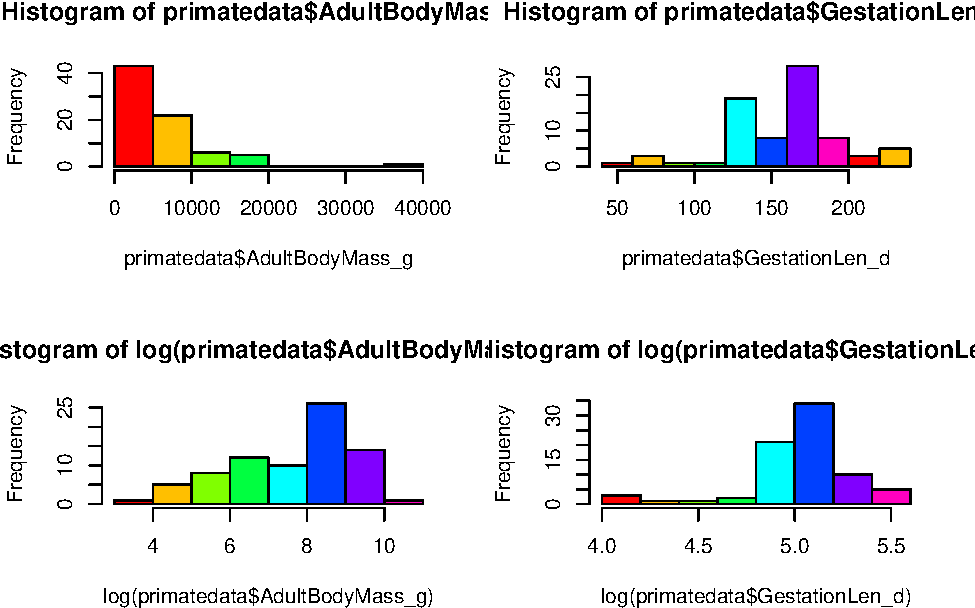
\includegraphics{macro-module_files/figure-latex/unnamed-chunk-85-1.pdf}

\begin{Shaded}
\begin{Highlighting}[]
\KeywordTok{par}\NormalTok{(}\DataTypeTok{mfrow =} \KeywordTok{c}\NormalTok{(}\DecValTok{1}\NormalTok{,}\DecValTok{1}\NormalTok{)) }\CommentTok{# So we can go back to 1 plot}
\end{Highlighting}
\end{Shaded}

OK let's do a linear regression of log gestation length against log
adult body mass:

\begin{Shaded}
\begin{Highlighting}[]
\NormalTok{model.ols <-}\StringTok{ }\KeywordTok{lm}\NormalTok{(}\KeywordTok{log}\NormalTok{(GestationLen_d) ~}\StringTok{ }\KeywordTok{log}\NormalTok{(AdultBodyMass_g), }\DataTypeTok{data =} \NormalTok{primatedata)}
\KeywordTok{summary}\NormalTok{(model.ols)}
\end{Highlighting}
\end{Shaded}

\begin{verbatim}
## 
## Call:
## lm(formula = log(GestationLen_d) ~ log(AdultBodyMass_g), data = primatedata)
## 
## Residuals:
##      Min       1Q   Median       3Q      Max 
## -0.61614 -0.08279  0.00646  0.11414  0.50558 
## 
## Coefficients:
##                      Estimate Std. Error t value Pr(>|t|)    
## (Intercept)            4.1037     0.1108  37.042  < 2e-16 ***
## log(AdultBodyMass_g)   0.1204     0.0141   8.544  1.1e-12 ***
## ---
## Signif. codes:  0 '***' 0.001 '**' 0.01 '*' 0.05 '.' 0.1 ' ' 1
## 
## Residual standard error: 0.1977 on 75 degrees of freedom
## Multiple R-squared:  0.4933, Adjusted R-squared:  0.4865 
## F-statistic: 73.01 on 1 and 75 DF,  p-value: 1.097e-12
\end{verbatim}

The slope is positive (\texttt{0.1204\ ±\ 0.0141}), and very significant
(note that R can't display values lower than \textless{}2e-16 which is
why it shows up so often).

We can also plot the regression line on a scatter plot:

\begin{Shaded}
\begin{Highlighting}[]
\KeywordTok{plot}\NormalTok{(}\KeywordTok{log}\NormalTok{(GestationLen_d) ~}\StringTok{ }\KeywordTok{log}\NormalTok{(AdultBodyMass_g), }\DataTypeTok{data =} \NormalTok{primatedata)}
\KeywordTok{abline}\NormalTok{(model.ols)}
\end{Highlighting}
\end{Shaded}

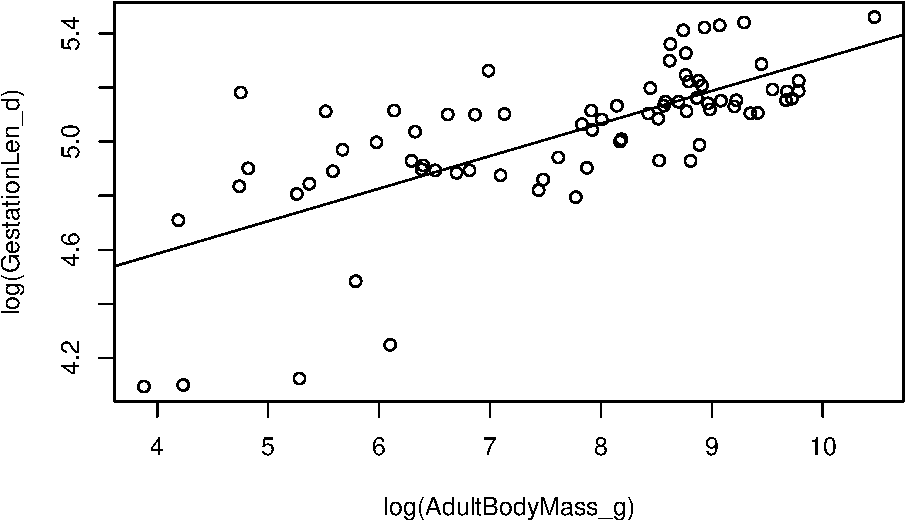
\includegraphics{macro-module_files/figure-latex/unnamed-chunk-87-1.pdf}

We can look at the phylogenetic pseudoreplication problem on the graph
by colouring the points by family.

\begin{Shaded}
\begin{Highlighting}[]
\KeywordTok{plot}\NormalTok{(}\KeywordTok{log}\NormalTok{(GestationLen_d) ~}\StringTok{ }\KeywordTok{log}\NormalTok{(AdultBodyMass_g), }\DataTypeTok{data =} \NormalTok{primatedata, }\DataTypeTok{col =} \NormalTok{primatedata$Family, }\DataTypeTok{pch =} \DecValTok{16}\NormalTok{)}
\end{Highlighting}
\end{Shaded}

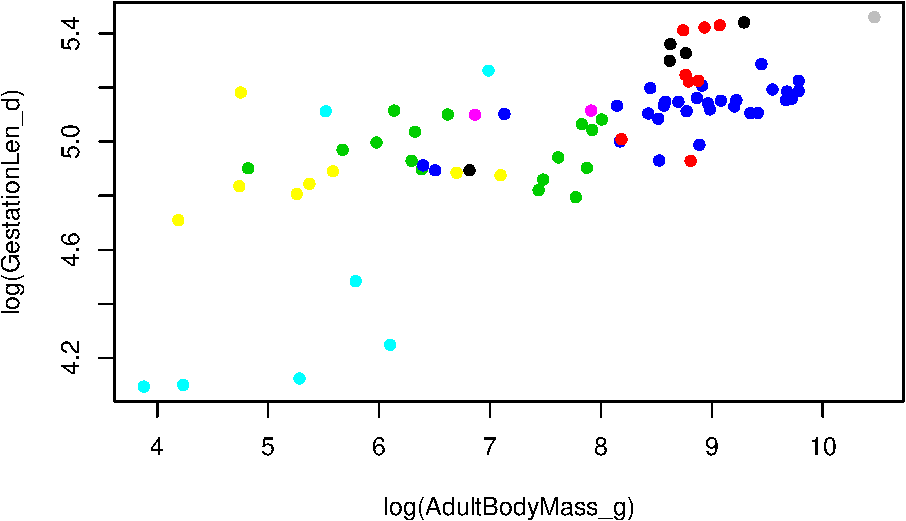
\includegraphics{macro-module_files/figure-latex/unnamed-chunk-88-1.pdf}

\begin{center}\rule{0.5\linewidth}{\linethickness}\end{center}

\section{Phylogenetic generalized least squares models
(PGLS)}\label{phylogenetic-generalized-least-squares-models-pgls}

There are several ways of accounting for phylogenetic non independence
in your analyses. Here we will just cover one - phylogenetic generalized
least squares (PGLS). Another popular earlier method is independent
contrasts. This method is really similar to PGLS, in fact it is just a
special kind of PGLS where \(\lambda\) is equal to 1. PGLS offers some
important advantages over independent contrasts. The model of trait
evolution can be more flexible i.e., it can depart from a strict
Brownian motion process (\(\lambda\) or K = 1). Different scaling
parameters (\(\lambda\), \(\kappa\), and \(\delta\)) can be incorporated
in the analysis, which can significantly improve the fit of the data to
the model and thus also improve the estimation of the trait correlation.
Another advantage of PGLS is that the intercept of the regression is not
forced to be zero.

To perform PGLS models in R, \texttt{caper} requires you to first
combine the phylogeny and data into one object using the function
\texttt{comparative.data}.

Note that \texttt{vcv\ =\ TRUE} stores a variance covariance matrix of
your tree (you will need this for the \texttt{pgls} function).
\texttt{na.omit\ =\ FALSE} stops the function from removing species
without data for all variables. \texttt{warn.dropped\ =\ TRUE} will tell
you if any species are not in both the tree and the data and are
therefore dropped from the comparative data object. Here we won't drop
any species because we already did this using \texttt{name.check}.

\begin{Shaded}
\begin{Highlighting}[]
\NormalTok{primate <-}\StringTok{ }\KeywordTok{comparative.data}\NormalTok{(}\DataTypeTok{phy =} \NormalTok{primatetree, }\DataTypeTok{data =} \NormalTok{primatedata, }
                            \DataTypeTok{names.col =} \NormalTok{Binomial, }\DataTypeTok{vcv =} \OtherTok{TRUE}\NormalTok{, }
                            \DataTypeTok{na.omit =} \OtherTok{FALSE}\NormalTok{, }\DataTypeTok{warn.dropped =} \OtherTok{TRUE}\NormalTok{)}
\end{Highlighting}
\end{Shaded}

If you do need to drop species, this function will give a warning
telling you that some species have been dropped. You can view the
dropped species using:

\begin{Shaded}
\begin{Highlighting}[]
\NormalTok{primate$dropped$tips}
\end{Highlighting}
\end{Shaded}

\begin{verbatim}
## character(0)
\end{verbatim}

\begin{Shaded}
\begin{Highlighting}[]
\NormalTok{primate$dropped$unmatched.rows}
\end{Highlighting}
\end{Shaded}

\begin{verbatim}
## character(0)
\end{verbatim}

\textbf{Always} make sure you check the list of dropped species is what
you expected, it often reveals typos in your species names, or
mismatches in taxonomies used etc.

The function for PGLS analyses in \texttt{caper} is \texttt{pgls}. To
fit a model which uses the Maximum Likelihood (ML) estimate of
\(\lambda\) we use the following code:

\begin{Shaded}
\begin{Highlighting}[]
\NormalTok{model.pgls <-}\StringTok{ }\KeywordTok{pgls}\NormalTok{(}\KeywordTok{log}\NormalTok{(GestationLen_d) ~}\StringTok{ }\KeywordTok{log}\NormalTok{(AdultBodyMass_g), }\DataTypeTok{data =} \NormalTok{primate, }\DataTypeTok{lambda =} \StringTok{"ML"}\NormalTok{)}
\KeywordTok{summary}\NormalTok{(model.pgls)}
\end{Highlighting}
\end{Shaded}

\begin{verbatim}
## 
## Call:
## pgls(formula = log(GestationLen_d) ~ log(AdultBodyMass_g), data = primate, 
##     lambda = "ML")
## 
## Residuals:
##       Min        1Q    Median        3Q       Max 
## -0.098899 -0.011661  0.003082  0.017758  0.075133 
## 
## Branch length transformations:
## 
## kappa  [Fix]  : 1.000
## lambda [ ML]  : 0.892
##    lower bound : 0.000, p = 1.1435e-14
##    upper bound : 1.000, p = 0.00046393
##    95.0% CI   : (0.753, 0.967)
## delta  [Fix]  : 1.000
## 
## Coefficients:
##                      Estimate Std. Error t value  Pr(>|t|)    
## (Intercept)          4.290229   0.160355 26.7546 < 2.2e-16 ***
## log(AdultBodyMass_g) 0.104864   0.019628  5.3426 9.479e-07 ***
## ---
## Signif. codes:  0 '***' 0.001 '**' 0.01 '*' 0.05 '.' 0.1 ' ' 1
## 
## Residual standard error: 0.0261 on 75 degrees of freedom
## Multiple R-squared: 0.2757,  Adjusted R-squared: 0.266 
## F-statistic: 28.54 on 1 and 75 DF,  p-value: 9.479e-07
\end{verbatim}

As well as the standard regression outputs, the output includes the
estimated ML value of \(\lambda\) (0.892) and p values from likelihood
ratio tests showing whether the ML \(\lambda\) is significantly
different from 0 or 1. \(\kappa\) and \(\delta\) are also tree
transformations which can improve the fit of the data to the tree. It is
also possible to use \texttt{pgls} to optimise \(\kappa\) or \(\delta\)
(using kappa = ``ML'' or delta = ``ML'' instead of lambda = ``ML'' in
the code above). We will not cover this today. Note that optimizing more
than one of these parameters at the same time is not advisable because
it would be impossible to interpret the results!

We can also plot the results as follows:

\begin{Shaded}
\begin{Highlighting}[]
\KeywordTok{plot}\NormalTok{(}\KeywordTok{log}\NormalTok{(GestationLen_d) ~}\StringTok{ }\KeywordTok{log}\NormalTok{(AdultBodyMass_g), }\DataTypeTok{data =} \NormalTok{primatedata)}
\KeywordTok{abline}\NormalTok{(model.pgls)}
\end{Highlighting}
\end{Shaded}

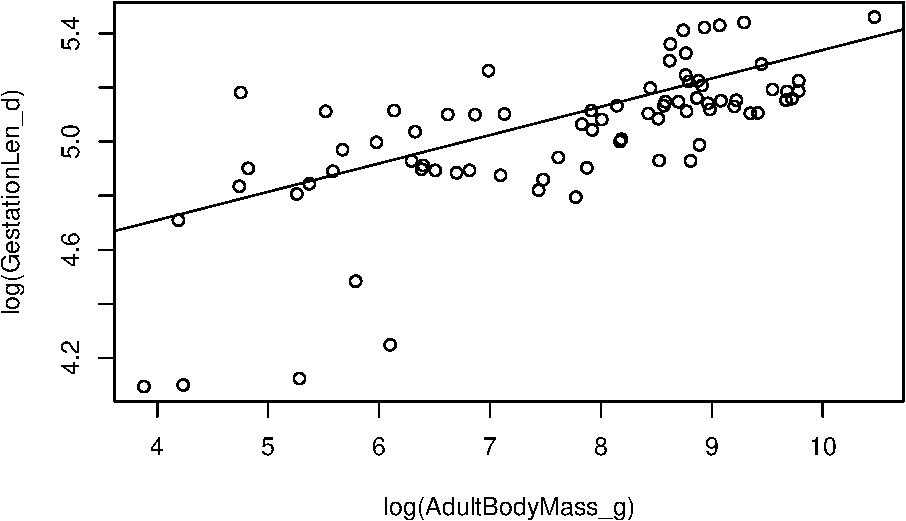
\includegraphics{macro-module_files/figure-latex/unnamed-chunk-92-1.pdf}

Sometimes you will find that \texttt{pgls} will not work and you get an
\texttt{optim\ error}. This is much more common when using a Mac. To fix
it all you need to do is change the bounds (upper and lower values) on
the parameter being optimized, in this case \(\lambda\). Just change the
lower bound of \(\lambda\) to something a little bigger than 1e-6 until
it works. For example:

\begin{Shaded}
\begin{Highlighting}[]
\NormalTok{model.pgls2 <-}\StringTok{ }\KeywordTok{pgls}\NormalTok{(}\KeywordTok{log}\NormalTok{(GestationLen_d) ~}\StringTok{ }\KeywordTok{log}\NormalTok{(AdultBodyMass_g), }\DataTypeTok{data =} \NormalTok{primate, }\DataTypeTok{lambda =} \StringTok{"ML"}\NormalTok{, }\DataTypeTok{bounds =} \KeywordTok{list}\NormalTok{(}\DataTypeTok{lambda =} \KeywordTok{c}\NormalTok{(}\FloatTok{1e-05}\NormalTok{, }\DecValTok{1}\NormalTok{)))}
\end{Highlighting}
\end{Shaded}

\subsection{\texorpdfstring{Likelihood profiles for \(\lambda\) in PGLS
models}{Likelihood profiles for \textbackslash{}lambda in PGLS models}}\label{likelihood-profiles-for-lambda-in-pgls-models}

You can look at the likelihood profiles for branch length
transformations in PGLS models using \texttt{pgls.profile}:

\begin{Shaded}
\begin{Highlighting}[]
\NormalTok{lambda.profile <-}\StringTok{ }\KeywordTok{pgls.profile}\NormalTok{(model.pgls, }\StringTok{"lambda"}\NormalTok{)}
\KeywordTok{plot}\NormalTok{(lambda.profile)}
\end{Highlighting}
\end{Shaded}

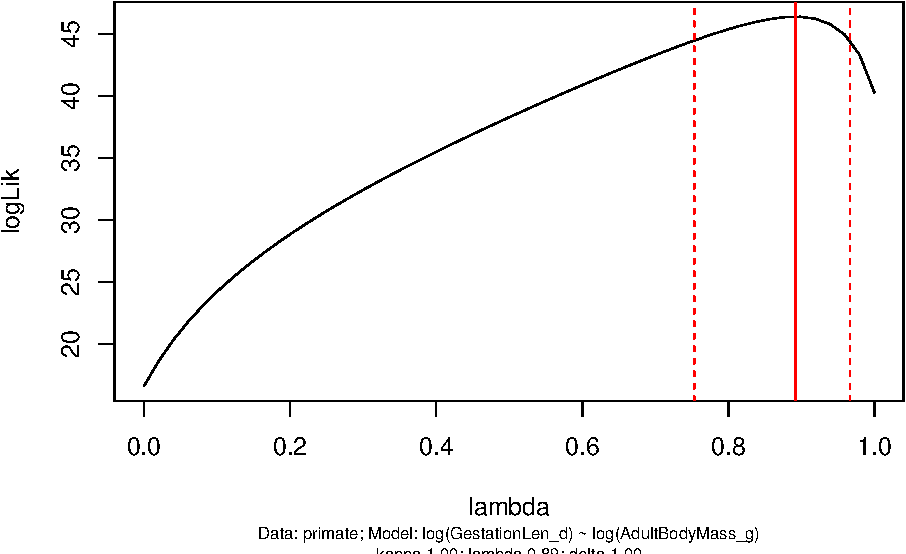
\includegraphics{macro-module_files/figure-latex/unnamed-chunk-94-1.pdf}

This graph shows the likelihood profile of \(\lambda\) in our model.
Ideally you want a line with an obvious peak/optimum like this, rather
than a flat line which would suggest \(\lambda\) could be anything. You
can see that the optimum (the peak of the curve) is at 0.892 as
estimated in our PGLS model. The dotted red lines are the 95\%
confidence intervals on \(\lambda\) for our model. \texttt{pgls.confint}
prints out these numbers in \texttt{\$ci.val}

\begin{Shaded}
\begin{Highlighting}[]
\KeywordTok{pgls.confint}\NormalTok{(model.pgls, }\StringTok{"lambda"}\NormalTok{)$ci.val}
\end{Highlighting}
\end{Shaded}

\begin{verbatim}
## [1] 0.753434 0.966543
\end{verbatim}

\textbf{Big problems with small datasets} You will often find strange
\(\lambda\) profiles when you don't have a lot of species in your data,
because \(\lambda\) (and Blomberg's K - see below) has very low power to
detect phylogenetic signal for less than 20-30 data points (see
Freckleton et al. 2002 Am Nat). This means that using PGLS on small
datasets is tricky - you almost always get ML \(\lambda\) of zero but
the \(\lambda\) profile will show a pretty flat likelihood surface.
Unfortunately people often forget to look at the \(\lambda\) profile so
erroneously conclude that there is no phylogenetic autocorrelation in
their data.

\textbf{Generally I'd say don't use small datasets, however, this seems
unavoidable in some fields.} Therefore my advice is to (only in this
situation!) ignore one of Freckleton's deadly sins (2009, JEB) and
report the results from an OLS model (equivalent of PGLS with
\(\lambda\) = 0) and also report the results from a PGLS model with
\(\lambda\) set to 1 (equivalent to independent contrasts). This problem
comes up every year and current consensus among the PCM community is
that this is best solution at present, if collecting more data is really
not an option!

\textbf{To set \(\lambda\) to 1 you just replace ``ML'' with 1}

\begin{Shaded}
\begin{Highlighting}[]
\NormalTok{model.pgls3 <-}\StringTok{ }\KeywordTok{pgls}\NormalTok{(}\KeywordTok{log}\NormalTok{(GestationLen_d) ~}\StringTok{ }\KeywordTok{log}\NormalTok{(AdultBodyMass_g), }\DataTypeTok{data =} \NormalTok{primate, }\DataTypeTok{lambda =} \DecValTok{1}\NormalTok{)}
\end{Highlighting}
\end{Shaded}

\subsection{Model diagnostics for PGLS
models}\label{model-diagnostics-for-pgls-models}

You should always check model diagnostic plots whenever you fit a model
in R to check that your data meet the assumptions of the model. The
method for this in PGLS is the same for OLS, independent contrasts and
PGLS models (though the graphs are slightly different). To get model
diagnostic plots for PGLS:

\begin{Shaded}
\begin{Highlighting}[]
\KeywordTok{par}\NormalTok{(}\DataTypeTok{mfrow =} \KeywordTok{c}\NormalTok{(}\DecValTok{2}\NormalTok{, }\DecValTok{2}\NormalTok{))}
\KeywordTok{plot}\NormalTok{(model.pgls)}
\end{Highlighting}
\end{Shaded}

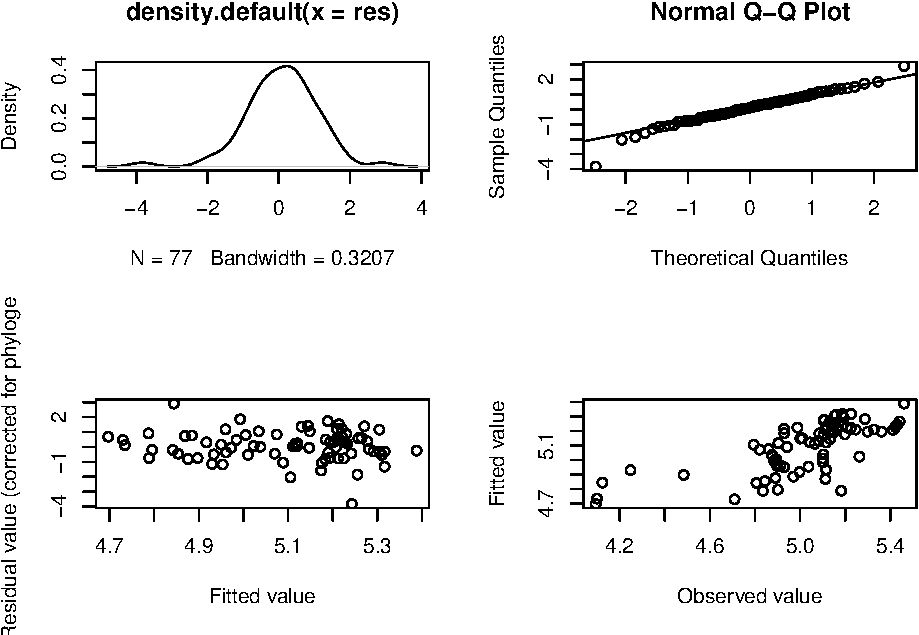
\includegraphics{macro-module_files/figure-latex/unnamed-chunk-97-1.pdf}

\begin{Shaded}
\begin{Highlighting}[]
\KeywordTok{par}\NormalTok{(}\DataTypeTok{mfrow =} \KeywordTok{c}\NormalTok{(}\DecValTok{1}\NormalTok{, }\DecValTok{1}\NormalTok{))}
\end{Highlighting}
\end{Shaded}

Without going into the statistical details (and if you've no idea what
these plots are for I suggest looking this up online or in a stats
textbook), what you are looking for in these plots is:

\begin{enumerate}
\def\labelenumi{\arabic{enumi}.}
\tightlist
\item
  In plot one you shouldn't see any data with a studentized residual
  \textgreater{} \(\pm\) 3. Any species with such large residuals should
  be removed as these outliers may overly influence the results of the
  regression (see Jones and Purvis 1997). Often these are the result of
  measurement error associated with species pairs joined by very short
  branches. You should generally report results with and without
  outliers unless the results remain qualitatively the same.
\item
  The points of the Q-Q plot (plot 2) should approximately fall on the
  line. This tests for normality of residuals, one of the assumptions of
  linear models
\item
  Plots 3 and 4 should show a fairly random scattering of points. You
  want to avoid any clear patterns. The first is related to the
  systematic component of the model - any pattern here suggests that the
  model has not been correctly specified. The second is to test the
  assumption that variances are equal (homoscedascity).
\end{enumerate}

It takes practice to know what is ``good'', ``bad'' and ``acceptable''
with these plots. I would say the plots above are fine, but there appear
to be a couple of data points with studentized residuals \textgreater{}
\(\pm\) 3 in plot 1 that should be removed, or at least checked for
errors.

\begin{center}\rule{0.5\linewidth}{\linethickness}\end{center}

\section{Estimating phylogenetic signal for one
variable}\label{estimating-phylogenetic-signal-for-one-variable}

\subsection{\texorpdfstring{Pagel's \(\lambda\) (Pagel 1997/1999,
Freckleton et al
2002)}{Pagel's \textbackslash{}lambda (Pagel 1997/1999, Freckleton et al 2002)}}\label{pagels-lambda-pagel-19971999-freckleton-et-al-2002}

Phylogenetic signal is merely the pattern where close relatives have
more similar trait values than more distant relatives (see Kamilar and
Cooper 2013). Often people will mention that they ``corrected for
phylogeny'' because of the phylogenetic signal in their variables.
However, we \textbf{do not} correct for phylogeny because our variables
show phylogenetic signal. We account for phylogenetic non-independence
because the \textbf{residuals} from our models show phylogenetic signal
(see Revell 2010). \(\lambda\) shown in PGLS models above is the
\(\lambda\) for the model residuals \textbf{not} the individual
variables.

Sometimes however, you might be interested in the phylogenetic signal of
just one trait. \(\lambda\) is really easy to estimate using
\texttt{caper}. To do this for log GestationLen\_d:

\begin{Shaded}
\begin{Highlighting}[]
\NormalTok{lambdaGL <-}\StringTok{ }\KeywordTok{pgls}\NormalTok{(}\KeywordTok{log}\NormalTok{(GestationLen_d) ~}\StringTok{ }\DecValTok{1}\NormalTok{, }\DataTypeTok{data =} \NormalTok{primate, }\DataTypeTok{lambda =} \StringTok{"ML"}\NormalTok{)}
\KeywordTok{summary}\NormalTok{(lambdaGL)}
\end{Highlighting}
\end{Shaded}

\begin{verbatim}
## 
## Call:
## pgls(formula = log(GestationLen_d) ~ 1, data = primate, lambda = "ML")
## 
## Residuals:
##       Min        1Q    Median        3Q       Max 
## -0.128354 -0.014460  0.001389  0.017572  0.074329 
## 
## Branch length transformations:
## 
## kappa  [Fix]  : 1.000
## lambda [ ML]  : 0.948
##    lower bound : 0.000, p = < 2.22e-16
##    upper bound : 1.000, p = 0.030039
##    95.0% CI   : (0.859, 0.996)
## delta  [Fix]  : 1.000
## 
## Coefficients:
##             Estimate Std. Error t value  Pr(>|t|)    
## (Intercept)  5.00514    0.11723  42.694 < 2.2e-16 ***
## ---
## Signif. codes:  0 '***' 0.001 '**' 0.01 '*' 0.05 '.' 0.1 ' ' 1
## 
## Residual standard error: 0.0334 on 76 degrees of freedom
## Multiple R-squared:     0,   Adjusted R-squared:     0 
## F-statistic:   NaN on 0 and 76 DF,  p-value: NA
\end{verbatim}

Note that by replacing the explanatory variables with 1 you are just
investigating the relationship between log gestation length and the
phylogeny. Thus the \(\lambda\) value is the \(\lambda\) estimate for
log GestationLen\_d and the p values are from likelihood ratio tests
showing whether the ML \(\lambda\) is significantly different from 0 (no
phylogenetic signal) or 1 (the expectation under Brownian motion).

\begin{center}\rule{0.5\linewidth}{\linethickness}\end{center}

\subsection{Blomberg's K (Blomberg et al
2003)}\label{blombergs-k-blomberg-et-al-2003}

To estimate Blomberg's K we use the \texttt{Kcalc} function in
\texttt{picante}. First you need to set up a new vector with the values
for the variable you are interested in, here the log of gestation
length, and with a names attribute with the names of your species. Here
I'll call this vector \texttt{lngest}.

\begin{Shaded}
\begin{Highlighting}[]
\NormalTok{lngest <-}\StringTok{ }\KeywordTok{log}\NormalTok{(primatedata$GestationLen_d)}
\KeywordTok{names}\NormalTok{(lngest) <-}\StringTok{ }\NormalTok{primatedata$Binomial}
\end{Highlighting}
\end{Shaded}

We can then calculate K for log gestation length:

\begin{Shaded}
\begin{Highlighting}[]
\KeywordTok{Kcalc}\NormalTok{(lngest[primatetree$tip.label], primatetree)}
\end{Highlighting}
\end{Shaded}

\begin{verbatim}
##           [,1]
## [1,] 0.7757771
\end{verbatim}

\texttt{Kcalc} (and \texttt{phylosignal}) require the trait data to be
in the same order as the tree tip labels.
\texttt{lngest{[}primatetree\$tip.label{]}} selects gestation lengths
from the species in the same order as they are in the tree (square
brackets \texttt{{[}\ {]}} are used in R to subset data).

K for log gestation length is 0.7758. As with \(\lambda\) above, we're
interested in whether the value of K is significantly different from
what we'd expect by chance. We can do this using the function
\texttt{phylosignal}. This function randomly assigns the trait values to
the species and then calculates K. This is repeated 1000 times (if
\texttt{reps\ =\ 1000}) and the observed value of K is then compared to
the randomized values to determine its significance.

\begin{Shaded}
\begin{Highlighting}[]
\KeywordTok{phylosignal}\NormalTok{(lngest[primatetree$tip.label], primatetree, }\DataTypeTok{reps =} \DecValTok{1000}\NormalTok{)}
\end{Highlighting}
\end{Shaded}

\begin{verbatim}
##           K PIC.variance.obs PIC.variance.rnd.mean PIC.variance.P
## 1 0.7757771      0.001660764            0.01194213    0.000999001
##   PIC.variance.Z
## 1       -2.26644
\end{verbatim}

In this case the observed K is significantly higher than the random
values of K (\texttt{PIC.variance.P} \textless{} 0.001).

\emph{Note this is a randomization test so your output here will not be
identical to mine.}

\begin{center}\rule{0.5\linewidth}{\linethickness}\end{center}

\section{References}\label{references-1}

\begin{itemize}
\tightlist
\item
  Arnold, C., L. J. Matthews, and C. L. Nunn. 2010. The 10ktrees
  website: a new online resource for primate phylogeny. Evolutionary
  Anthropology: Issues, News, and Reviews 19:114--118.
\item
  Blomberg, S. P., T. Garland, and A. R. Ives. 2003. Testing for
  phylogenetic signal in comparative data: behavioral traits are more
  labile. Evolution 57:717--745.
\item
  Freckleton, R. P., P. H. Harvey, and M. Pagel. 2002. Phylogenetic
  analysis and comparative data: a test and review of evidence. The
  American Naturalist 160:712-726.
\item
  Freckleton, R. P. (2009) The seven deadly sins of comparative
  analysis. Journal of Evolutionary Biology, 22, 1367--1375.
\item
  Jones, K. E., J. Bielby, M. Cardillo, S. A. Fritz, J. O'Dell, C. D. L.
  Orme, K. Safi, W. Sechrest, E. H. Boakes, C. Carbone, et al. 2009.
  Pantheria: a species-level database of life history, ecology, and
  geography of extant and recently extinct mammals: Ecological archives
  e090-184. Ecology 90:2648--2648.
\item
  Kamilar, J. M., \& Cooper, N. 2013. Phylogenetic signal in primate
  behaviour, ecology and life history. Phil. Trans. R. Soc. B,
  368(1618), 20120341.
\item
  Pagel, M. 1999. Inferring the historical patterns of biological
  evolution. Nature, 401(6756), 877-884.
\item
  Revell, L. J. 2010. Phylogenetic signal and linear regression on
  species data. Methods in Ecology and Evolution, 1, 319-329.
\end{itemize}

\subsection{Extra Reading}\label{extra-reading-1}

\begin{itemize}
\tightlist
\item
  Losos, J.B. (2011) Seeing the forest for the trees: the limitations of
  phylogenies in comparative biology. The American Naturalist, 177,
  709--727.
\end{itemize}

\chapter{Macroevolutionary models in R: Part 1 - continuous
traits}\label{macroevolutionary-models-in-r-part-1---continuous-traits}

The aims of this practical are to learn how to use R to fit
macroevolutionary models in R to continuous traits.

We will be using the evolution of magical creature life-history
variables as an example. The data includes body mass (average adult size
at rest) in kg, social status (1 = solitary, 2 = social), habitat (1 =
terrestrial, 2 = aquatic, 3 = volant) and magical power (in thaum - with
thanks to Terry Pratchett for the units). These data are invented, so
please don't get too upset if I've misclassified anything!

\textbf{REMEMBER}

\begin{itemize}
\tightlist
\item
  Download all of the data for the practical into a folder somewhere on
  your computer.
\item
  Set your working directory to this folder.
\item
  Start a new script for this practical.
\end{itemize}

You will also need to install the following packages:

\begin{itemize}
\tightlist
\item
  \texttt{ape}
\item
  \texttt{geiger}
\item
  \texttt{OUwie}
\end{itemize}

This practical is in two parts, Part 2 deals with discrete traits.

\begin{center}\rule{0.5\linewidth}{\linethickness}\end{center}

\section{Preparing for the analysis}\label{preparing-for-the-analysis-1}

\subsection{Load packages, read in the data and the
tree}\label{load-packages-read-in-the-data-and-the-tree}

This is the same as we did in the PGLS practical, so I won't give
detailed instructions here.

\begin{Shaded}
\begin{Highlighting}[]
\CommentTok{# Load packages}
\KeywordTok{library}\NormalTok{(ape)}
\KeywordTok{library}\NormalTok{(geiger)}
\KeywordTok{library}\NormalTok{(OUwie)}
\end{Highlighting}
\end{Shaded}

\begin{Shaded}
\begin{Highlighting}[]
\CommentTok{# Read in data}
\NormalTok{magicaldata <-}\StringTok{ }\KeywordTok{read.csv}\NormalTok{(}\StringTok{"magicalcreatures.csv"}\NormalTok{)}
\CommentTok{# Check data is loaded correctly}
\KeywordTok{str}\NormalTok{(magicaldata)}
\end{Highlighting}
\end{Shaded}

\begin{verbatim}
## 'data.frame':    30 obs. of  5 variables:
##  $ Species     : Factor w/ 30 levels "Acromantula",..: 22 24 19 5 7 16 21 25 30 29 ...
##  $ BodySize_kg : num  1.5 50 0.5 100 8000 1 2.5 6 800 600 ...
##  $ SocialStatus: int  2 2 2 1 1 2 2 1 1 2 ...
##  $ Habitat     : int  1 1 2 1 3 1 1 3 3 3 ...
##  $ Magic_thaum : num  106.3 86.7 98.6 57 131.9 ...
\end{verbatim}

\begin{Shaded}
\begin{Highlighting}[]
\CommentTok{# Read in tree}
\NormalTok{magicaltree <-}\StringTok{ }\KeywordTok{read.nexus}\NormalTok{(}\StringTok{"magicaltree.nex"}\NormalTok{) }
\CommentTok{# Check tree is loaded correctly}
\KeywordTok{str}\NormalTok{(magicaltree)}
\end{Highlighting}
\end{Shaded}

\begin{verbatim}
## List of 4
##  $ edge       : int [1:52, 1:2] 28 29 30 31 31 30 32 33 33 34 ...
##  $ edge.length: num [1:52] 136.86 65.69 97 2.92 2.92 ...
##  $ Nnode      : int 26
##  $ tip.label  : chr [1:27] "Doxie" "Bowtruckle" "Hinkypuff" "Grindylow" ...
##  - attr(*, "class")= chr "phylo"
##  - attr(*, "order")= chr "cladewise"
\end{verbatim}

\subsection{Modify the tree and data so they can be used in the
analyses.}\label{modify-the-tree-and-data-so-they-can-be-used-in-the-analyses.}

Again we did this in the PGLS practical. Please remind yourself of what
these steps are needed for.

\begin{Shaded}
\begin{Highlighting}[]
\CommentTok{# Ensure tree is fully bifurcating}
\NormalTok{magicaltree <-}\StringTok{ }\KeywordTok{multi2di}\NormalTok{(magicaltree) }

\CommentTok{# Replace spaces with underscores in the species names}
\NormalTok{magicaldata$Species <-}\StringTok{ }\KeywordTok{gsub}\NormalTok{(}\StringTok{" "}\NormalTok{, }\StringTok{"_"}\NormalTok{, magicaldata$Species)}

\CommentTok{# Add species names to row names}
\KeywordTok{row.names}\NormalTok{(magicaldata) <-}\StringTok{ }\NormalTok{magicaldata$Species}
\end{Highlighting}
\end{Shaded}

For some weird reason the \texttt{geiger} function we need
(\texttt{treedata} see below) won't work if you input a dataset with
variables that are characters i.e.~words or letters. Our taxonomic
variable Species is a character so we need to exclude it from the data.
Note for your own data you'd need to remove all character variables (or
recode them as 0,12 etc.). We will do this by making a new dataset
called magicaldata2.

\begin{Shaded}
\begin{Highlighting}[]
\NormalTok{magicaldata2 <-}\StringTok{ }\NormalTok{magicaldata[, }\DecValTok{2}\NormalTok{:}\DecValTok{5}\NormalTok{]}
\end{Highlighting}
\end{Shaded}

Here the {[} {]} tells R we want to subset the dataset. R data frames
are always described by {[}X,Y{]} where X is rows and Y is columns. So
{[}1, 1{]} will select the entry in the first column and the first row
of the data frame. {[}, 2:2{]} selects all rows but only columns 2 to 5.
These are the columns containing our numeric variables.

We then need to match the species in tree to those in the dataset as in
the PGLS practical. \textbf{Note that we are using \texttt{magicaldata2}
here.}

\begin{Shaded}
\begin{Highlighting}[]
\NormalTok{match.species <-}\StringTok{ }\KeywordTok{treedata}\NormalTok{(magicaltree, magicaldata2)}

\NormalTok{mytree <-}\StringTok{ }\NormalTok{match.species$phy}
\NormalTok{mydata <-}\StringTok{ }\NormalTok{match.species$data}
\end{Highlighting}
\end{Shaded}

\begin{center}\rule{0.5\linewidth}{\linethickness}\end{center}

\section{Models of continuous trait
evolution}\label{models-of-continuous-trait-evolution}

For fitting models of evolution to continuous data we will use the
\texttt{fitContinuous} function in the R package \texttt{geiger}.
\texttt{fitContinuous} is a likelihood based method, so the output will
give the maximum likelihood (ML) estimates of the parameters. Bayesian
methods are becoming preferred for these kinds of analyses and
\texttt{fitContinuousMCMC} will perform these analyses. However, due to
time constraints we will not cover this function. As an example, let's
look at the evolution of \texttt{log(body\ size)} in magical creatures.
We'll fit three evolutionary models -- the Brownian motion (BM) model,
the Ornstein-Uhlenbeck (OU) model and the Early Burst (EB) model.
\texttt{fitContinuous} can also fit several other models. For more
details look at the help file by typing: \texttt{?fitContinuous}

\subsection{The Brownian motion (BM
model)}\label{the-brownian-motion-bm-model}

The Brownian motion model (Cavalli-Sforza and Edwards, 1967;
Felsenstein, 1973) is assumed to be the underlying mode of evolution in
the majority of phylogenetic comparative methods (though this assumption
is rarely tested; Freckleton and Harvey 2006). In the model, a trait
\(X\) evolves at random at a rate \(\sigma\):

\(dX(t) = \sigma dW(t)\)

where \(W(t)\) is a white noise function and is a random variate drawn
from a normal distribution with mean 0 and variance \(\sigma^2\). This
model assumes that there is no overall drift in the direction of
evolution (hence the expectation of \(W(t)\) is zero) and that the rate
of evolution is constant. Because the direction of change in trait
values at each step is random, Brownian motion is often described as a
``random walk'' (note that you can also fit models where \(W(t)\) is not
zero and there is drift in the direction of evolution. This is known as
the drift model, or Brownian motion with a trend. We will not cover this
here).

The model assumes the correlation structure among trait values is
proportional to the extent of shared ancestry for pairs of species. This
means that close relatives will be more similar in their trait values
than more distant relatives. It also means that variance in the trait
will increase (linearly) in proportion to time. The model has two
parameters, the Brownian rate parameter, \(\sigma^2\) and the state of
the root at time zero, \(X(0)\). \texttt{fitContinuous} estimates
\(\sigma^2\) and \(X(0)\). Note that \(\sigma^2\) can be used as a
measure of the rate of trait evolution (Cooper and Purvis, 2010; Cooper
et al., 2011).

\subsection{The Ornstein-Uhlenbeck (OU)
model}\label{the-ornstein-uhlenbeck-ou-model}

The Ornstein-Uhlenbeck (OU) model (Hansen, 1997; Butler and King, 2004)
is a random walk where trait values are pulled back towards some
``optimal'' value with an attraction strength proportional to the
parameter \(\alpha\). The model has the following form:

\(dX(t) = -\alpha(X(t) - \mu) + \sigma dW(t)\)

Note that this model has two parameters in addition to those of the
Brownian model, \(\alpha\) and \(\mu\). The parameter m is a long-term
mean, and it is assumed that species evolve around this value.
\(\alpha\) is the strength of evolutionary force that returns traits
back towards the long-term mean if they evolve away from it. \(\alpha\)
is sometimes referred to as the ``rubber band'' parameter because of the
way it forces traits back towards \(\mu\). The OU model was introduced
to population genetics by Lande (1976) to model stabilizing selection in
which the mean was recast as a fitness optimum on an adaptive landscape.
The process operating in comparative data is analogous, although clearly
is not stabilizing selection (despite being sometimes referred to as
such). The model has four parameters, the Brownian rate parameter,
\(\sigma^2\), the state of the root at time zero, \(X(0)\), the
attraction strength or ``rubber band'' parameter, \(\alpha\), and the
long-term mean, \(\mu\). \texttt{fitContinuous} estimates \(\sigma^2\),
\(X(0)\), and \(\alpha\). It does not estimate \(\mu\) but in this
implementation of the model, \(\mu\) is equivalent to \(X(0)\). Note
that if \(\alpha\) is close to zero then evolution is approximately
Brownian.

\subsection{The Early Burst (EB) model}\label{the-early-burst-eb-model}

The Early Burst (EB) model (Harmon et al. 2010, also called the ACDC
model; Blomberg et al. 2003) is a Brownian motion/random walk model
where the rate of evolution decreases exponentially through time under
the model:

\(r(t) = \sigma^2e(at)\)

Where \(r(t)\) is the rate of evolution at time \(t\), \(\sigma^2\) is
the initial value of the Brownian rate parameter, i.e.~the initial rate
of evolution, \(a\) is the rate change parameter, and \(t\) is time. The
value of \(a\) is generally less than or equal to 0 (note that you can
force \(a\) to be greater than zero by changing the bounds - see section
3.4 - however, this will only work if you have fossil species in your
data; Slater et al. 2012). When a is negative, rates of evolution
decrease through time. The model fits traits where diversification
occurs most rapidly early in a lineage and slows as the lineage
approaches the present, so that subclades tend to retain their
differences through time. This is consistent with a clade radiating
adaptively into a fixed set of niches and has been used as evidence of
niche-filling modes of evolution (Harmon et al., 2010; Cooper and
Purvis, 2010). The model has three parameters, the Brownian rate
parameter, \(\sigma^2\), the state of the root at time zero, \(X(0)\),
and the rate of change parameter, \(a\). \texttt{fitContinuous}
estimates \(\sigma^2\), \(X(0)\) and \(a\). Note that if \(a\) is close
to zero then evolution is approximately Brownian. Note that although
many people report a values when reporting the results of fitting an
Early Burst model, it is often more intuitive to report the rate
half-life, \(t_{\frac{1}{2}}\) (Slater and Pennell, 2014). This is
calculated as:

\(t_{\frac{1}{2}} = \frac{log(2)}{|a|}\)

It can be interpreted as the time it takes for the rate of evolution of
the trait to halve.

\section{\texorpdfstring{Fitting the models using
\texttt{fitContinuous}}{Fitting the models using fitContinuous}}\label{fitting-the-models-using-fitcontinuous}

First we will fit a Brownian motion (BM) model to log(body mass):

\begin{Shaded}
\begin{Highlighting}[]
\NormalTok{BM <-}\StringTok{ }\KeywordTok{fitContinuous}\NormalTok{(mytree, }\KeywordTok{log}\NormalTok{(mydata[,}\StringTok{"BodySize_kg"}\NormalTok{]), }\DataTypeTok{model =} \KeywordTok{c}\NormalTok{(}\StringTok{"BM"}\NormalTok{))}
\end{Highlighting}
\end{Shaded}

To look at the output type:

\begin{Shaded}
\begin{Highlighting}[]
\NormalTok{BM}
\end{Highlighting}
\end{Shaded}

\begin{verbatim}
## GEIGER-fitted comparative model of continuous data
##  fitted 'BM' model parameters:
##  sigsq = 2.207510
##  z0 = 4.304110
## 
##  model summary:
##  log-likelihood = -98.541855
##  AIC = 201.083711
##  AICc = 201.583711
##  free parameters = 2
## 
## Convergence diagnostics:
##  optimization iterations = 100
##  failed iterations = 0
##  frequency of best fit = 1.00
## 
##  object summary:
##  'lik' -- likelihood function
##  'bnd' -- bounds for likelihood search
##  'res' -- optimization iteration summary
##  'opt' -- maximum likelihood parameter estimates
\end{verbatim}

The maximum likelihood estimates (\texttt{lnL}) of the model parameters
are found near the top of the output. In a Brownian motion (BM) model we
estimate the Brownian rate parameter, \(\sigma^2\) or \texttt{sigsq} in
the output above, which is \texttt{2.208} and the value of the trait at
the root of the tree, \(X(0)\) or \texttt{z0} in the output above, which
is \texttt{4.304}. Other useful things in the output are the
maximum-likelihood estimate (\texttt{lnL}) of the model
(log-likelihood), the Akaike Information Criterion (\texttt{AIC}),
sample-size corrected AIC (\texttt{AICc}) and the number of model
parameters (free parameters) also known as \(k\) in the literature. We
will return to the AIC values below.

To fit an Ornstein-Uhlenbeck model to log(body mass) we only need to
change the model in the formula we used above:

\begin{Shaded}
\begin{Highlighting}[]
\NormalTok{OU <-}\StringTok{ }\KeywordTok{fitContinuous}\NormalTok{(mytree, }\KeywordTok{log}\NormalTok{(mydata[,}\StringTok{"BodySize_kg"}\NormalTok{]), }\DataTypeTok{model =} \KeywordTok{c}\NormalTok{(}\StringTok{"OU"}\NormalTok{))}
\end{Highlighting}
\end{Shaded}

To look at the output type:

\begin{Shaded}
\begin{Highlighting}[]
\NormalTok{OU}
\end{Highlighting}
\end{Shaded}

\begin{verbatim}
## GEIGER-fitted comparative model of continuous data
##  fitted 'OU' model parameters:
##  alpha = 2.718282
##  sigsq = 60.982369
##  z0 = 3.203383
## 
##  model summary:
##  log-likelihood = -70.843002
##  AIC = 147.686004
##  AICc = 148.729482
##  free parameters = 3
## 
## Convergence diagnostics:
##  optimization iterations = 100
##  failed iterations = 0
##  frequency of best fit = 0.05
## 
##  object summary:
##  'lik' -- likelihood function
##  'bnd' -- bounds for likelihood search
##  'res' -- optimization iteration summary
##  'opt' -- maximum likelihood parameter estimates
\end{verbatim}

As above, the maximum likelihood estimates (\texttt{lnL}) of the model
parameters are found near the top of the output. In an
Ornstein-Uhlenbeck (OU) model we estimate the Brownian rate parameter,
\(\sigma^2\) or \texttt{sigsq} in the output above, the value of the
trait at the root of the tree, \(X(0)\) or \texttt{z0} in the output
above, and the selection strength parameter, \(\alpha\) or
\texttt{alpha} in the output above. As \texttt{alpha\ =\ 2.718} here, it
suggests that there is evolution towards a body mass optimum.

Finally, to fit an Early Burst (EB) model to log(body mass):

\begin{Shaded}
\begin{Highlighting}[]
\NormalTok{EB <-}\StringTok{ }\KeywordTok{fitContinuous}\NormalTok{(mytree, }\KeywordTok{log}\NormalTok{(mydata[,}\StringTok{"BodySize_kg"}\NormalTok{]), }\DataTypeTok{model =} \KeywordTok{c}\NormalTok{(}\StringTok{"EB"}\NormalTok{))}
\end{Highlighting}
\end{Shaded}

To look at the output type:

\begin{Shaded}
\begin{Highlighting}[]
\NormalTok{EB}
\end{Highlighting}
\end{Shaded}

\begin{verbatim}
## GEIGER-fitted comparative model of continuous data
##  fitted 'EB' model parameters:
##  a = -0.000001
##  sigsq = 2.208177
##  z0 = 4.304129
## 
##  model summary:
##  log-likelihood = -98.542390
##  AIC = 203.084780
##  AICc = 204.128258
##  free parameters = 3
## 
## Convergence diagnostics:
##  optimization iterations = 100
##  failed iterations = 0
##  frequency of best fit = 0.58
## 
##  object summary:
##  'lik' -- likelihood function
##  'bnd' -- bounds for likelihood search
##  'res' -- optimization iteration summary
##  'opt' -- maximum likelihood parameter estimates
\end{verbatim}

As above, the maximum likelihood estimates (\texttt{lnL}) of the model
parameters are found near the top of the output. In an Early Burst (EB)
model we estimate the Brownian rate parameter, \(\sigma^2\) or
\texttt{sigsq} in the output above, the value of the trait at the root
of the tree, \(X(0)\) or \texttt{z0} in the output above, and the rate
of change parameter, \(a\). Here \texttt{a} is very close to 0
indicating that the rate of log(body mass) evolution in magical
creatures has not decreased through time.

We can also extract the rate half-life, \(t_{\frac{1}{2}}\), for this
model as follows:

\begin{Shaded}
\begin{Highlighting}[]
\KeywordTok{log}\NormalTok{(}\DecValTok{2}\NormalTok{)/}\KeywordTok{abs}\NormalTok{(EB$opt$a)}
\end{Highlighting}
\end{Shaded}

\begin{verbatim}
## [1] 693142.8
\end{verbatim}

For these data, the rate half-life is almost 700,000 time units, much
greater than the total time represented on the tree! This means over the
course of magical creature evolution, body size rate has not halved
(yet).

\subsection{Comparing models of
evolution}\label{comparing-models-of-evolution}

Often we want to know which of the models fits our variable best. We can
use \texttt{fitContinuous} to fit the models we are interested in and
can then compare them using AIC. We can extract the AICs from the models
we fitted above as follows:

\begin{Shaded}
\begin{Highlighting}[]
\NormalTok{BM$opt$aic}
\end{Highlighting}
\end{Shaded}

\begin{verbatim}
## [1] 201.0837
\end{verbatim}

\begin{Shaded}
\begin{Highlighting}[]
\NormalTok{OU$opt$aic}
\end{Highlighting}
\end{Shaded}

\begin{verbatim}
## [1] 147.686
\end{verbatim}

\begin{Shaded}
\begin{Highlighting}[]
\NormalTok{EB$opt$aic}
\end{Highlighting}
\end{Shaded}

\begin{verbatim}
## [1] 203.0848
\end{verbatim}

The ``best'' model is the one with the smallest AIC, in this case the OU
model. There is much debate about how big of a difference in AIC values
can be classed as substantial improvement to a model fit (it usually
ranges from 2-10 AIC units). Generally we use 4 units, so EB probably
doesn't fit substantially better than BM, but OU is substantially better
than BM and EB.

Alternatively we can use \(\Delta\)AIC or AIC weights to compare our
models using the following code and the \texttt{geiger} function
\texttt{aicw}:

\begin{Shaded}
\begin{Highlighting}[]
\NormalTok{aic.scores <-}\StringTok{ }\KeywordTok{setNames}\NormalTok{(}\KeywordTok{c}\NormalTok{(BM$opt$aic, OU$opt$aic, EB$opt$aic), }\KeywordTok{c}\NormalTok{(}\StringTok{"BM"}\NormalTok{,}\StringTok{"OU"}\NormalTok{,}\StringTok{"EB"}\NormalTok{))}
\KeywordTok{aicw}\NormalTok{(aic.scores)}
\end{Highlighting}
\end{Shaded}

\begin{verbatim}
##         fit    delta            w
## BM 201.0837 53.39771 2.540009e-12
## OU 147.6860  0.00000 1.000000e+00
## EB 203.0848 55.39878 9.339176e-13
\end{verbatim}

\texttt{aicw} outputs the AIC (\texttt{fit}), \(\Delta\)AIC
(\texttt{delta}) and AIC weights (\texttt{w}) for each of the models we
fitted. The best model is the model with \(\Delta\)AIC = 0 or with AICw
closest to 1. Using \(\Delta\)AIC we can conclude that the OU model is
the best fit to the data.

\subsection{Problems with convergence and
bounds}\label{problems-with-convergence-and-bounds}

Above we have mentioned the default bounds on each parameter. Sometimes
these need to be changed because the model will not converge. This
happens when the likelihood surface has long flat ridges that cause the
likelihood search to get ``stuck'' (this is particularly common under
the OU model). You can change bounds with the bounds argument in
\texttt{fitContinuous}. Several bounds can be given at a time e.g.
\texttt{bounds\ =\ list(sigsq\ =\ c(0,\ 0.1),\ alpha\ =\ c(0,\ 1))}
would constrain both the \(\sigma^2\) and \(\alpha\) parameters.

For example, if an OU model keeps getting stuck you could try changing
the lower bound on \(\alpha\):

\begin{Shaded}
\begin{Highlighting}[]
\NormalTok{OU <-}\StringTok{ }\KeywordTok{fitContinuous}\NormalTok{(}\DataTypeTok{phy =} \NormalTok{mytree, }\DataTypeTok{dat =} \KeywordTok{log}\NormalTok{(mydata[,}\StringTok{"BodySize_kg"}\NormalTok{]), }\DataTypeTok{model =} \KeywordTok{c}\NormalTok{(}\StringTok{"OU"}\NormalTok{), }
                    \DataTypeTok{bounds =} \KeywordTok{list}\NormalTok{(}\DataTypeTok{alpha =} \KeywordTok{c}\NormalTok{(}\FloatTok{0.01}\NormalTok{, }\DecValTok{1}\NormalTok{)))}
\end{Highlighting}
\end{Shaded}

This example gives a warning message because \texttt{alpha} is over 1,
so when we make the upper bound smaller the method ends up giving us
this value instead because it's as close to 1 as we are allowing the
model to go.

\begin{center}\rule{0.5\linewidth}{\linethickness}\end{center}

\section{References}\label{references-2}

\begin{itemize}
\tightlist
\item
  Blomberg, S. P., T. Garland, and A. R. Ives. 2003. Testing for
  phylogenetic signal in comparative data: behavioral traits are more
  labile. Evolution 57:717--745.
\item
  Butler, M. A. and A. A. King. 2004. Phylogenetic comparative analysis:
  a modeling approach for adaptive evolution. The American Naturalist
  164:683--695.
\item
  Cavalli-Sforza, L. L. and A. W. Edwards. 1967. Phylogenetic analysis.
  models and estimation procedures. American Journal of Human Genetics
  19:233.
\item
  Cooper, N., R. P. Freckleton, and W. Jetz. 2011. Phylogenetic
  conservatism of environmental niches in mammals. Proceedings of the
  Royal Society B: Biological Sciences 278:2384--2391.
\item
  Cooper, N. and A. Purvis. 2010. Body size evolution in mammals:
  complexity in tempo and mode.The American Naturalist 175:727--738.
\item
  Cooper, N., Thomas, G.H., Venditti, C., Meade, A. \& Freckleton, R.P.
  (2016b) A cautionary note on the use of ornstein-uhlenbeck models in
  macroevolutionary studies. Biological Journal of the Linnaean Society
\item
  Felsenstein, J. 1973. Maximum likelihood and minimum-steps methods for
  estimating evolutionary trees from data on discrete characters.
  Systematic Biology 22:240--249.
\item
  Freckleton, R. P. and P. H. Harvey. 2006. Detecting non-brownian trait
  evolution in adaptive radiations. PLoS Biology 4:e373.
\item
  Hansen, T. F. 1997. Stabilizing selection and the comparative analysis
  of adaptation. Evolution Pages 1341--1351.
\item
  Harmon, L. J., J. B. Losos, T. Jonathan Davies, R. G. Gillespie, J. L.
  Gittleman, W. Bryan Jennings, K. H. Kozak, M. A. McPeek, F.
  Moreno-Roark, T. J. Near, et al. 2010. Early bursts of body size and
  shape evolution are rare in comparative data. Evolution 64:2385--2396.
\item
  Lande, R. 1976. Natural selection and random genetic drift in
  phenotypic evolution. Evolution 30:314--334.
\item
  Slater, G. J., L. J. Harmon, and M. E. Alfaro. 2012. Integrating
  fossils with molecular phylogenies improves inference of trait
  evolution. Evolution 66:3931--3944.
\item
  Slater, G. J. and M.W. Pennell. 2014. Robust regression and posterior
  predictive simulation increase power to detect early bursts of trait
  evolution. Systematic Biology 63:293--308.
\end{itemize}

\chapter{Macroevolutionary models in R: Part 2 - discrete
traits}\label{macroevolutionary-models-in-r-part-2---discrete-traits}

The aims of this practical are to learn how to use R to fit
macroevolutionary models in R to discrete traits.

We will be using the evolution of magical creature life-history
variables as an example. The data includes body mass (average adult size
at rest) in kg, social status (1 = solitary, 2 = social), habitat (1 =
terrestrial, 2 = aquatic, 3 = volant) and magical power (in thaum - with
thanks to Terry Pratchett for the units). These data are invented, so
please don't get too upset if I've misclassified anything!

\textbf{REMEMBER}

\begin{itemize}
\tightlist
\item
  Download all of the data for the practical into a folder somewhere on
  your computer.
\item
  Set your working directory to this folder.
\item
  Start a new script for this practical.
\end{itemize}

You will also need to install the following packages:

\begin{itemize}
\tightlist
\item
  \texttt{ape}
\item
  \texttt{geiger}
\item
  \texttt{OUwie}
\end{itemize}

This is Part 2 of the ``Macroevolutionary models in R'' practical, so
you can skip through the set up if you're just carrying on from that.

This handout borrows heavily from a Linnaean Society workshop I ran with
Graham Slater in 2014. Many thanks to Graham for his invaluable input.

\begin{center}\rule{0.5\linewidth}{\linethickness}\end{center}

\section{Preparing for the analysis}\label{preparing-for-the-analysis-2}

\subsection{Load packages, read in the data and the
tree}\label{load-packages-read-in-the-data-and-the-tree-1}

This is the same as we did in the PGLS practical, so I won't give
detailed instructions here.

\begin{Shaded}
\begin{Highlighting}[]
\CommentTok{# Load packages}
\KeywordTok{library}\NormalTok{(ape)}
\KeywordTok{library}\NormalTok{(geiger)}
\KeywordTok{library}\NormalTok{(OUwie)}
\end{Highlighting}
\end{Shaded}

\begin{Shaded}
\begin{Highlighting}[]
\CommentTok{# Read in data}
\NormalTok{magicaldata <-}\StringTok{ }\KeywordTok{read.csv}\NormalTok{(}\StringTok{"magicalcreatures.csv"}\NormalTok{)}
\CommentTok{# Check data is loaded correctly}
\KeywordTok{str}\NormalTok{(magicaldata)}
\end{Highlighting}
\end{Shaded}

\begin{verbatim}
## 'data.frame':    30 obs. of  5 variables:
##  $ Species     : Factor w/ 30 levels "Acromantula",..: 22 24 19 5 7 16 21 25 30 29 ...
##  $ BodySize_kg : num  1.5 50 0.5 100 8000 1 2.5 6 800 600 ...
##  $ SocialStatus: int  2 2 2 1 1 2 2 1 1 2 ...
##  $ Habitat     : int  1 1 2 1 3 1 1 3 3 3 ...
##  $ Magic_thaum : num  106.3 86.7 98.6 57 131.9 ...
\end{verbatim}

\begin{Shaded}
\begin{Highlighting}[]
\CommentTok{# Read in tree}
\NormalTok{magicaltree <-}\StringTok{ }\KeywordTok{read.nexus}\NormalTok{(}\StringTok{"magicaltree.nex"}\NormalTok{) }
\CommentTok{# Check tree is loaded correctly}
\KeywordTok{str}\NormalTok{(magicaltree)}
\end{Highlighting}
\end{Shaded}

\begin{verbatim}
## List of 4
##  $ edge       : int [1:52, 1:2] 28 29 30 31 31 30 32 33 33 34 ...
##  $ edge.length: num [1:52] 136.86 65.69 97 2.92 2.92 ...
##  $ Nnode      : int 26
##  $ tip.label  : chr [1:27] "Doxie" "Bowtruckle" "Hinkypuff" "Grindylow" ...
##  - attr(*, "class")= chr "phylo"
##  - attr(*, "order")= chr "cladewise"
\end{verbatim}

\subsection{Modify the tree and data so they can be used in the
analyses.}\label{modify-the-tree-and-data-so-they-can-be-used-in-the-analyses.-1}

Again we did this in the PGLS practical. Please remind yourself of what
these steps are needed for.

\begin{Shaded}
\begin{Highlighting}[]
\CommentTok{# Ensure tree is fully bifurcating}
\NormalTok{magicaltree <-}\StringTok{ }\KeywordTok{multi2di}\NormalTok{(magicaltree) }

\CommentTok{# Replace spaces with underscores in the species names}
\NormalTok{magicaldata$Species <-}\StringTok{ }\KeywordTok{gsub}\NormalTok{(}\StringTok{" "}\NormalTok{, }\StringTok{"_"}\NormalTok{, magicaldata$Species)}

\CommentTok{# Add species names to row names}
\KeywordTok{row.names}\NormalTok{(magicaldata) <-}\StringTok{ }\NormalTok{magicaldata$Species}
\end{Highlighting}
\end{Shaded}

For some weird reason the \texttt{geiger} function we need
(\texttt{treedata} see below) won't work if you input a dataset with
variables that are characters i.e.~words or letters. Our taxonomic
variable Species is a character so we need to exclude it from the data.
Note for your own data you'd need to remove all character variables (or
recode them as 0,12 etc.). We will do this by making a new dataset
called magicaldata2.

\begin{Shaded}
\begin{Highlighting}[]
\NormalTok{magicaldata2 <-}\StringTok{ }\NormalTok{magicaldata[, }\DecValTok{2}\NormalTok{:}\DecValTok{5}\NormalTok{]}
\end{Highlighting}
\end{Shaded}

Here the {[} {]} tells R we want to subset the dataset. R data frames
are always described by {[}X,Y{]} where X is rows and Y is columns. So
{[}1, 1{]} will select the entry in the first column and the first row
of the data frame. {[}, 2:2{]} selects all rows but only columns 2 to 5.
These are the columns containing our numeric variables.

We then need to match the species in tree to those in the dataset as in
the PGLS practical. \textbf{Note that we are using \texttt{magicaldata2}
here.}

\begin{Shaded}
\begin{Highlighting}[]
\NormalTok{match.species <-}\StringTok{ }\KeywordTok{treedata}\NormalTok{(magicaltree, magicaldata2)}

\NormalTok{mytree <-}\StringTok{ }\NormalTok{match.species$phy}
\NormalTok{mydata <-}\StringTok{ }\NormalTok{match.species$data}
\end{Highlighting}
\end{Shaded}

\begin{center}\rule{0.5\linewidth}{\linethickness}\end{center}

\section{Fitting models of evolution to discrete data (regime dependent
evolution)}\label{fitting-models-of-evolution-to-discrete-data-regime-dependent-evolution}

In the previous section we saw how to fit three models of trait
evolution to continuous variables. Although the evolutionary modes seem
quite different, all are similar in that the evolutionary process is
constant over the entire clade, i.e., all branches are evolving at the
same rate (in BM), drawn to the same trait value with the same strength
(OU) or decline in rate at the same time-dependent pace (EB). Often, we
want to relax this assumption. Members of our clade might belong to one
of a set of ecological regimes, for example dietary niches or locomotor
modes, and we might hypothesize that there are different evolutionary
rates or different optimal trait values for each of these regimes. In
this section, we'll look at how to fit these kinds of models using the
\texttt{OUwie} package.

First we will look at how to reconstruct the evolutionary history of a
discrete trait. Then we will use \texttt{OUwie} to allow rates and
optimal trait values for a continuously valued trait, like body size, to
vary, based on that discrete trait.

Here we will use the discrete variable \texttt{SocialStatus} from our
magical creature dataset. Any species with a social group size of 1 is
solitary (SocialStatus = 1), while any species with a group size greater
than 1 is social (SocialStatus = 2).

We can visualize these variables on our tree by plotting them with
colors. We'll use light blue for solitary and plum for social. Because
our states are coded as ``1'' and ``2'', we can use a little trick to
get the appropriate colors by indexing a vector of ``lightblue'' and
``plum''. We first need to make sure teh species in our data are in the
same order as those in the tree.

\begin{Shaded}
\begin{Highlighting}[]
\CommentTok{# Reorder the data so it's the same order as in the tree}
\NormalTok{mydata <-}\StringTok{ }\NormalTok{mydata[}\KeywordTok{match}\NormalTok{(mytree$tip.label,}\KeywordTok{rownames}\NormalTok{(mydata)),]}

\CommentTok{# Create a vector of two colours}
\NormalTok{social.colors <-}\StringTok{ }\KeywordTok{c}\NormalTok{(}\StringTok{"lightblue"}\NormalTok{, }\StringTok{"plum"}\NormalTok{)}

\CommentTok{# Plot the tree, add coloured tip labels and a legend}
\KeywordTok{plot}\NormalTok{(mytree, }\DataTypeTok{cex =} \FloatTok{0.5}\NormalTok{)}
\KeywordTok{tiplabels}\NormalTok{(}\DataTypeTok{pch =} \DecValTok{16}\NormalTok{, }\DataTypeTok{col =} \NormalTok{social.colors[mydata[,}\StringTok{"SocialStatus"}\NormalTok{]])}
\KeywordTok{legend}\NormalTok{(}\StringTok{"bottomleft"}\NormalTok{,}\DataTypeTok{legend=}\KeywordTok{c}\NormalTok{(}\StringTok{"solitary"}\NormalTok{, }\StringTok{"social"}\NormalTok{), }
       \DataTypeTok{pch =} \DecValTok{15}\NormalTok{, }\DataTypeTok{col=}\KeywordTok{c}\NormalTok{(}\StringTok{"lightblue"}\NormalTok{, }\StringTok{"plum"}\NormalTok{), }\DataTypeTok{bty =} \StringTok{"n"}\NormalTok{)}
\end{Highlighting}
\end{Shaded}

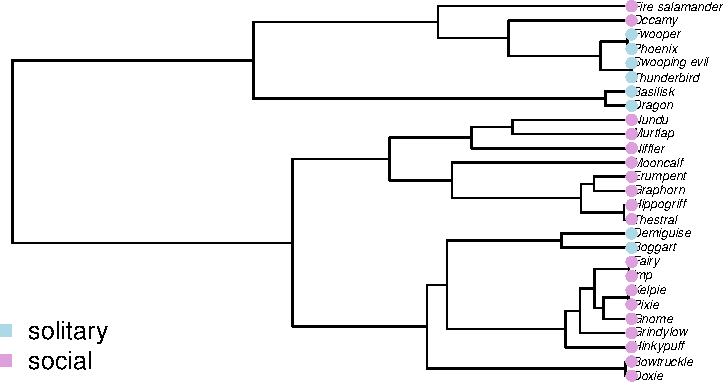
\includegraphics{macro-module_files/figure-latex/unnamed-chunk-124-1.pdf}

You'll see that solitary behavior seems to be more restricted in its
distribution. Most solitary magicals are bird or reptile like. From the
distribution on the phylogeny, we might guess that solitary behavior is
the ancestral state. This is exactly what we need to know in order to
test whether evolutionary modes for body size vary for solitary vs
social magical creatures. But before we can infer ancestral states, we
need to chose the most appropriate model of social evolution.

There are several ways of mapping social status onto the tree but
probably the most straightforward is to use an ancestral state
estimation. We will estimate ancestral states for each node under a
Markov model, pick the state with the highest marginal likelihood, and
then assign that as the node state.

Unfortunately, just like rates can vary for continuous traits, so they
can vary for discrete traits, and this can impact our ancestral state
estimation. Fortunately, it's straightforward to test for this kind of
heterogeneity using the \texttt{fitDiscrete} function in the
\texttt{geiger} package.

\section{Models of discrete trait
evolution}\label{models-of-discrete-trait-evolution}

\subsection{Mk1 -- all rates equal (ER)}\label{mk1-all-rates-equal-er}

The simplest Markov model we can fit to comparative data is an Mk1 model
-- M for Markov, k1 for \(k = 1\) or 1 parameter. The single parameter
of this model is a transition rate -- the rate at which states change.
Because we only have one rate, transitions between any pair of states
occur at the same rate and are therefore equally probable. We can
visualize the \(Q\) (rate) matrix for an Mk1 model like this:

\begin{longtable}[]{@{}llll@{}}
\toprule
- & 1 & 2 & 3\tabularnewline
\midrule
\endhead
1 & - & 1 & 1\tabularnewline
2 & 1 & - & 1\tabularnewline
3 & 1 & 1 & -\tabularnewline
\bottomrule
\end{longtable}

The off-diagonals are the transition rates from state 1 to 2, 1 to 3, 2
to 1 and so on (read rows then columns). We typically designate
individual transition rates in the form \(q_ij\), which means the rate
of going from state \(i\) to state \(j\). Here, the 1 in all
off-diagonal elements represents the fact that rates are the same
regardless of what state \(i\) and \(j\) are, and the direction of that
change. The diagonal elements \(q_ii\) give the rate of not changing and
are computed as the negative sum of the non-diagonal row elements. This
is so that the rows sum to zero.

If you're familiar with models of molecular evolution, you might know
this model better as the \textbf{Jukes-Cantor model}, where transition
rates = transversion rates.

\subsection{Mk -- symmetric rates (SYM)}\label{mk-symmetric-rates-sym}

We could add some complexity, and perhaps realism, by imagining that the
rate of change between any pair of states is the same regardless of
direction, but that the rate of change differs among states. Such a
model is referred to as a symmetric model, and has a \(Q\) matrix of the
form:

\begin{longtable}[]{@{}llll@{}}
\toprule
- & 1 & 2 & 3\tabularnewline
\midrule
\endhead
1 & - & 1 & 2\tabularnewline
2 & 1 & - & 3\tabularnewline
3 & 2 & 3 & -\tabularnewline
\bottomrule
\end{longtable}

Here, \(q_{12} = q_{21}\) but this rate is allowed to be different from
\(q_{13}/q_{31}\) and from \(q_{23}/q_{32}\). The number of different
rates is three for \(S = 3\). However, if we were to add a fourth state,
the new number of rates would not be 4 but rather would be 6. This is
because there would now be 6 distinct off-diagonal elements present in
the upper or lower diagonals.

If you're more familiar with molecular models, this is how we get the
6-rate GTR (General Time Reversible) model:

\begin{longtable}[]{@{}lllll@{}}
\toprule
- & A & C & T & G\tabularnewline
\midrule
\endhead
A & - & 1 & 2 & 3\tabularnewline
C & 1 & - & 4 & 5\tabularnewline
T & 2 & 4 & - & 6\tabularnewline
G & 3 & 5 & 6 & -\tabularnewline
\bottomrule
\end{longtable}

Obviously, a symmetric model with only 2 states becomes an equal rates
(Mk1) model.

\subsection{Mk -- All Rates Different
(ARD)}\label{mk-all-rates-different-ard}

Finally, we can go crazy and allow all rates to be different. For
S-states, this would generate \(S^2\) S rates FIXXXXXX, which might be
crazy, depending on how many states you have. For completeness, the
\(Q\) matrix for an All Rates Different model would look like this:

\begin{longtable}[]{@{}llll@{}}
\toprule
- & 1 & 2 & 3\tabularnewline
\midrule
\endhead
1 & - & 1 & 2\tabularnewline
2 & 3 & - & 4\tabularnewline
3 & 5 & 6 & -\tabularnewline
\bottomrule
\end{longtable}

If you're more familiar with molecular models, then you'll be aware that
molecular folks don't do this because of potential over-fitting. This is
a very important point to consider. However, in comparative data, there
are three situations in which this model might realistically be a good
fit.

\begin{enumerate}
\def\labelenumi{\arabic{enumi}.}
\tightlist
\item
  An All Rates Different model might be a good fit if you have an
  especially large datasets that spans a variety of different states.
  For example, if you had a tree of all 64,000 plus vertebrates and
  wanted to examine transition rates among different dietary strategies,
  this model would be worth examining.
\item
  If you have strong reasons to suppose character states are not
  reversible, this is worth using. For example, complex structures like
  eyes or teeth tend not to reappear once lost so asymmetric models
  might be a better fit for these kinds of characters.
\item
  This model is also a good option when you only have two states but
  think rates back and forth might be different. In this latter
  situation, the All Rates Different model simply gives you two rates,
  which isn't really over-fitting.
\end{enumerate}

\section{\texorpdfstring{Fitting the models using
\texttt{fitDiscrete}}{Fitting the models using fitDiscrete}}\label{fitting-the-models-using-fitdiscrete}

Let's try these models with our magical creatures dataset using
\texttt{fitDiscrete}. We will investigate rates of change in social
status.

\begin{Shaded}
\begin{Highlighting}[]
\NormalTok{equal <-}\StringTok{ }\KeywordTok{fitDiscrete}\NormalTok{(mytree, mydata[ , }\StringTok{"SocialStatus"}\NormalTok{], }\DataTypeTok{model =} \StringTok{"ER"}\NormalTok{)}
\CommentTok{#sym <- fitDiscrete(mytree, mydata[ , "SocialStatus"], model = "SYM")}
\NormalTok{ard <-}\StringTok{ }\KeywordTok{fitDiscrete}\NormalTok{(mytree, mydata[ , }\StringTok{"SocialStatus"}\NormalTok{], }\DataTypeTok{model =} \StringTok{"ARD"}\NormalTok{)}
\end{Highlighting}
\end{Shaded}

Before moving on, note that the commented out fitting of the symmetric
model is on purpose. Why? Remember that we only have 2 states, solitary
and social. A symmetric model with 2 states is just an equal rates
model, so we can conveniently ignore it here. Let's look at the output
for the equal rates model:

\begin{Shaded}
\begin{Highlighting}[]
\NormalTok{equal}
\end{Highlighting}
\end{Shaded}

\begin{verbatim}
## GEIGER-fitted comparative model of discrete data
##  fitted Q matrix:
##                  1            2
##     1 -0.002247321  0.002247321
##     2  0.002247321 -0.002247321
## 
##  model summary:
##  log-likelihood = -8.815776
##  AIC = 19.631552
##  AICc = 19.791552
##  free parameters = 1
## 
## Convergence diagnostics:
##  optimization iterations = 100
##  failed iterations = 0
##  frequency of best fit = 1.00
## 
##  object summary:
##  'lik' -- likelihood function
##  'bnd' -- bounds for likelihood search
##  'res' -- optimization iteration summary
##  'opt' -- maximum likelihood parameter estimates
\end{verbatim}

This looks very similar to the output from \texttt{fitContinuous}. We've
got a model summary, with log likelihoods and AIC scores, convergence
diagnostics and an object summary. The only difference is the first
part, which gives us a fitted \(Q\) matrix, rather than a summary of
model parameters (the \(Q\) matrix \textbf{is} the model parameters).
This is an equal rates model, so the two off-diagonal elements are all
same, and the diagonals are the negative values of the rates (so rows
sum to zero).

By typing \texttt{ard}, we can look at the output for the
all-rates-different model:

\begin{Shaded}
\begin{Highlighting}[]
\NormalTok{ard}
\end{Highlighting}
\end{Shaded}

\begin{verbatim}
## GEIGER-fitted comparative model of discrete data
##  fitted Q matrix:
##                  1            2
##     1 -0.005617678  0.005617678
##     2  0.002368874 -0.002368874
## 
##  model summary:
##  log-likelihood = -8.634626
##  AIC = 21.269252
##  AICc = 21.769252
##  free parameters = 2
## 
## Convergence diagnostics:
##  optimization iterations = 100
##  failed iterations = 0
##  frequency of best fit = 0.43
## 
##  object summary:
##  'lik' -- likelihood function
##  'bnd' -- bounds for likelihood search
##  'res' -- optimization iteration summary
##  'opt' -- maximum likelihood parameter estimates
\end{verbatim}

It seems as though the rate of moving from solitary to social
(\texttt{0.005}) is slightly higher than the rate of going from social
to solitary (\texttt{0.002}). Based on our color-coordinated plot from
earlier, we might have predicted this to be the case.

Because the output of \texttt{equal} and \texttt{ard} are just like
\texttt{fitContinuous}, we can pull AICc values out and use them to
perform model selection:

\begin{Shaded}
\begin{Highlighting}[]
\NormalTok{aic.discrete <-}\StringTok{ }\KeywordTok{setNames}\NormalTok{(}\KeywordTok{c}\NormalTok{(equal$opt$aic, ard$opt$aic), }\KeywordTok{c}\NormalTok{(}\StringTok{"equal"}\NormalTok{, }\StringTok{"different"}\NormalTok{))}
\NormalTok{weights <-}\StringTok{ }\KeywordTok{aicw}\NormalTok{(aic.discrete)}
\NormalTok{weights}
\end{Highlighting}
\end{Shaded}

\begin{verbatim}
##                fit  delta         w
## equal     19.63155 0.0000 0.6939922
## different 21.26925 1.6377 0.3060078
\end{verbatim}

Based on AIC weights, which model should we prefer?

The all-rates-different model is less strongly supported
(\texttt{AICcW\ =\ 0.306}) than the equal rates model
(\texttt{AICcW\ =\ 0.694}). Now we can move forward with reconstructing
ancestral states under the preferred equal rates transition rate model.

\section{Ancestral state
reconstructions}\label{ancestral-state-reconstructions}

Ancestral state reconstruction is probably one of the most over-used and
uninformative methods in the phylogenetic comparative methods toolkit.
There are many reasons to be highly skeptical of ancestral state
estimates and interpretations of macroevolutionary patterns and process
that are based on them. However, if you want to know if evolutionary
tempo or mode have varied over clade history based on the state of a
discrete trait, you'll need to do it. We'll use \texttt{ape}'s
\texttt{ace} function here. There are other options out there, for
example in the \texttt{phytools} package. But \texttt{ace} will work for
our purposes.

To perform ancestral state estimation under the all-rates-different
model:

\begin{Shaded}
\begin{Highlighting}[]
\NormalTok{asr <-}\StringTok{ }\KeywordTok{ace}\NormalTok{(mydata[ , }\StringTok{"SocialStatus"}\NormalTok{], mytree, }\DataTypeTok{type =} \StringTok{"discrete"}\NormalTok{, }\DataTypeTok{model =} \StringTok{"ER"}\NormalTok{)}
\end{Highlighting}
\end{Shaded}

You might see an error message appear saying \texttt{NaNs\ produced}.

Don't worry about this -- it happens when rates for one transition are
particularly low but doesn't really affect our node state estimates. One
point to note here is that \texttt{ace} now defaults to a joint
estimation procedure, where the ancestral states are optimized based on
all information in the tree, not just the states at descendant tips.

We can access our ancestral states by typing:

\begin{Shaded}
\begin{Highlighting}[]
\NormalTok{asr$lik.anc}
\end{Highlighting}
\end{Shaded}

In this matrix, the columns correspond to nodes in the tree (the
numbering is off, as we'll see in a sec) and the two columns give the
scaled likelihoods that the node is in states 1 or 2. The scaled
likelihoods are like probabilities, so for the first node, we
reconstruct state 1 with probability = \texttt{0.3} and state 2 with
probability = \texttt{0.7} , but for node 2 the probability of state 1 =
\texttt{0.05} while that of state 2 = \texttt{0.95}. Scaled likelihoods
lend themselves very well to graphical display, so we can visualize
these states with pie charts on the tree we plotted earlier.

\begin{Shaded}
\begin{Highlighting}[]
\KeywordTok{plot}\NormalTok{(mytree, }\DataTypeTok{cex =} \FloatTok{0.5}\NormalTok{)}
\KeywordTok{nodelabels}\NormalTok{(}\DataTypeTok{pie =} \NormalTok{asr$lik.anc, }\DataTypeTok{piecol =} \NormalTok{social.colors, }\DataTypeTok{cex =} \FloatTok{0.5}\NormalTok{)}
\KeywordTok{tiplabels}\NormalTok{(}\DataTypeTok{pch =} \DecValTok{16}\NormalTok{, }\DataTypeTok{col =} \NormalTok{social.colors[mydata[,}\StringTok{"SocialStatus"}\NormalTok{]])}
\KeywordTok{legend}\NormalTok{(}\StringTok{"bottomleft"}\NormalTok{,}\DataTypeTok{legend=}\KeywordTok{c}\NormalTok{(}\StringTok{"solitary"}\NormalTok{, }\StringTok{"social"}\NormalTok{), }
       \DataTypeTok{pch =} \DecValTok{15}\NormalTok{, }\DataTypeTok{col=}\KeywordTok{c}\NormalTok{(}\StringTok{"lightblue"}\NormalTok{, }\StringTok{"plum"}\NormalTok{), }\DataTypeTok{bty =} \StringTok{"n"}\NormalTok{)}
\end{Highlighting}
\end{Shaded}

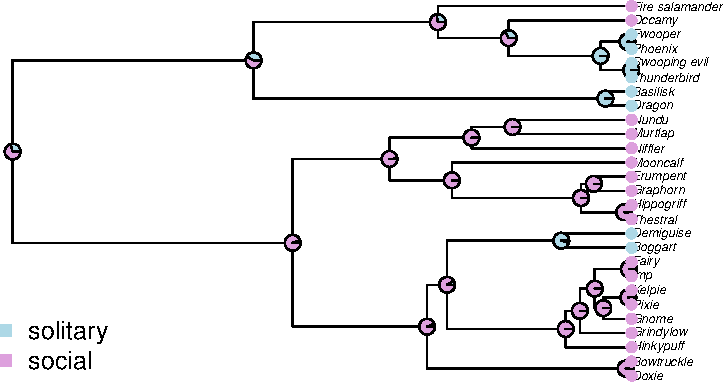
\includegraphics{macro-module_files/figure-latex/unnamed-chunk-131-1.pdf}

We reconstruct mostly social as the ancestral state for magical
creatures, but with multiple transitions to solitary behaviour. For our
next analyses though, we want to be able to extract the ``best'' state
for each node. We can do this quite easily with the data structure
\texttt{ace} gives us. First, we need to assign row names to our
ancestral states that actual correspond to node numbers. phylo--format
trees number nodes from \texttt{n+1} onwards, where \texttt{n} is the
number of taxa in the tree. So if there are 10 taxa, the root node is
11. Recall also that a fully bifurcating tree has \texttt{n\ -\ 1}
nodes. We can pull out the scaled likelihoods and number the rows
appropriately with two simple lines of code:

\begin{Shaded}
\begin{Highlighting}[]
\NormalTok{node.states <-}\StringTok{ }\NormalTok{asr$lik.anc}
\KeywordTok{rownames}\NormalTok{(node.states) <-}\StringTok{ }\KeywordTok{seq}\NormalTok{(}\DecValTok{1}\NormalTok{:}\KeywordTok{nrow}\NormalTok{(node.states)) +}\StringTok{ }\KeywordTok{length}\NormalTok{(mytree$tip.label)}
\NormalTok{node.states}
\end{Highlighting}
\end{Shaded}

\begin{verbatim}
##               1            2
## 28 2.951598e-01 7.048402e-01
## 29 5.176500e-02 9.482350e-01
## 30 6.723783e-02 9.327622e-01
## 31 2.788813e-05 9.999721e-01
## 32 8.812542e-02 9.118746e-01
## 33 1.121960e-03 9.988780e-01
## 34 9.481369e-05 9.999052e-01
## 35 1.180908e-05 9.999882e-01
## 36 1.291077e-05 9.999871e-01
## 37 5.096106e-07 9.999995e-01
## 38 4.892579e-07 9.999995e-01
## 39 9.532305e-01 4.676946e-02
## 40 6.559008e-03 9.934410e-01
## 41 4.773548e-03 9.952265e-01
## 42 1.850043e-04 9.998150e-01
## 43 4.923981e-06 9.999951e-01
## 44 5.791449e-05 9.999421e-01
## 45 2.257465e-03 9.977425e-01
## 46 1.779187e-03 9.982208e-01
## 47 4.183958e-01 5.816042e-01
## 48 9.983242e-01 1.675751e-03
## 49 2.750360e-01 7.249640e-01
## 50 3.333531e-01 6.666469e-01
## 51 9.925342e-01 7.465840e-03
## 52 1.000000e+00 3.595570e-08
## 53 9.999929e-01 7.068412e-06
\end{verbatim}

Now the rownumbers correspond to node numbers. This is useful. Now we'll
use a simple trick to extract the most likely states and assign them as
node values on our tree.

\begin{Shaded}
\begin{Highlighting}[]
\NormalTok{best <-}\StringTok{ }\KeywordTok{apply}\NormalTok{(node.states, }\DecValTok{1}\NormalTok{, which.max)}
\NormalTok{best}
\end{Highlighting}
\end{Shaded}

\begin{verbatim}
## 28 29 30 31 32 33 34 35 36 37 38 39 40 41 42 43 44 45 46 47 48 49 50 51 52 
##  2  2  2  2  2  2  2  2  2  2  2  1  2  2  2  2  2  2  2  2  1  2  2  1  1 
## 53 
##  1
\end{verbatim}

Now we have a named vector of ``best'' estimates of the node state. We
can assign these to the tree using the following line of code.

\begin{Shaded}
\begin{Highlighting}[]
\NormalTok{mytree$node.label <-}\StringTok{ }\NormalTok{best}
\NormalTok{mytree}
\end{Highlighting}
\end{Shaded}

\begin{verbatim}
## 
## Phylogenetic tree with 27 tips and 26 internal nodes.
## 
## Tip labels:
##  Doxie, Bowtruckle, Hinkypuff, Grindylow, Gnome, Pixie, ...
## Node labels:
##  2, 2, 2, 2, 2, 2, ...
## 
## Rooted; includes branch lengths.
\end{verbatim}

Now we have node labels associated with our magical tree that specify
which social regime each branch is evolving under. We're now ready to
move on to modeling state specific rate variation and adaptive optima,
using OUwie.

\section{\texorpdfstring{Fitting models using
\texttt{OUwie}}{Fitting models using OUwie}}\label{fitting-models-using-ouwie}

\texttt{OUwie} (pronounced Ow-EE) is a package written by Brian O'Meara
and Jeremy Beaulieu that performs maximum likelihood optimization of
Brownian motion and Ornstein-Uhlenbeck models. The models implemented
include the simple versions introduced earlier, but also include more
complex versions that allow model parameters (rates, selection, optima)
to vary among evolutionary regimes.

There are three things we need to fit an \texttt{OUwie} model. 1. A
phylogeny with internal nodes labeled with the ancestral selective
regimes - which we just did. 2. A dataset containing column entries in
the following order: i) species names, ii) current selective regime, and
iii) the continuous trait of interest. 3. The model we want to fit.

For the dataset all we need to do is make a dataframe with the relevant
information. Let's make it and look at the first few lines:

\begin{Shaded}
\begin{Highlighting}[]
\NormalTok{ouwie.data <-}\StringTok{ }\KeywordTok{data.frame}\NormalTok{(}\DataTypeTok{species =} \KeywordTok{rownames}\NormalTok{(mydata), }\DataTypeTok{regime =} \NormalTok{mydata[ , }\StringTok{"SocialStatus"}\NormalTok{],}
\DataTypeTok{trait =} \KeywordTok{log}\NormalTok{(mydata[ , }\StringTok{"BodySize_kg"}\NormalTok{]))}
\KeywordTok{head}\NormalTok{(ouwie.data)}
\end{Highlighting}
\end{Shaded}

\begin{verbatim}
##               species regime      trait
## Doxie           Doxie      2  0.4054651
## Bowtruckle Bowtruckle      2 -1.0498221
## Hinkypuff   Hinkypuff      2  0.0000000
## Grindylow   Grindylow      2 -0.5978370
## Gnome           Gnome      2  3.2188758
## Pixie           Pixie      2 -0.9162907
\end{verbatim}

Finally, we want to decide which model we're going to fit.

\subsection{Multi-rate Brownian motion
(BMS)}\label{multi-rate-brownian-motion-bms}

In \texttt{OUwie} a multi-rate BM model is coded as ``BMS''.

\begin{Shaded}
\begin{Highlighting}[]
\NormalTok{BMvariable <-}\StringTok{ }\KeywordTok{OUwie}\NormalTok{(mytree, ouwie.data, }\DataTypeTok{model =} \StringTok{"BMS"}\NormalTok{)}
\end{Highlighting}
\end{Shaded}

\begin{verbatim}
## Initializing... 
## Finished. Begin thorough search... 
## Finished. Summarizing results.
\end{verbatim}

Let's look at the results:

\begin{Shaded}
\begin{Highlighting}[]
\NormalTok{BMvariable}
\end{Highlighting}
\end{Shaded}

\begin{verbatim}
## 
## Fit
##        lnL      AIC     AICc model ntax
##  -72.14716 152.2943 154.1125   BMS   27
## 
## Rates
##                 1          2
## alpha          NA         NA
## sigma.sq 7.269257 0.09645345
## 
## Optima
##                 1        2
## estimate 18.71153 2.902904
## se       65.09904 3.209815
## 
## Arrived at a reliable solution
\end{verbatim}

The final line tells us that we arrived at a reliable solution -- that
is that the optimizer converged on a reliable set of parameter
estimates. The rest of the output includes log likelihood
(\texttt{LnL}), AIC (\texttt{AIC}) etc, the rates (including the alpha
parameters), and the optima. There are three main things to notice:

\begin{itemize}
\tightlist
\item
  You'll see here that there are \texttt{NAs} for alpha because this is
  a BM model, so there is no \(\alpha\) parameter to estimate.
\item
  The optima here correspond to the root state for species with state 1
  (solitary) or state 2 (social). It makes sense that the root state is
  higher for solitary species, as we know these can be huge (basilisks,
  dragons etc.) For OU models, these optima would be the adaptive
  optimal values of body mass for each of the two states.
\item
  The rates (\texttt{sigma.sq}) differ for regimes 1 and 2.
  Specifically, the rate for regime 1 (solitary) appears to be much
  higher that of regime 2 (social). So rates of body size evolution seem
  to be faster for solitary magical animals than for social magical
  animals, again this fits with our understanding of the data.
\end{itemize}

To know whether this difference is great enough for us to prefer this
model, we'd need to compare AIC scores, or something similar. We'll come
back to this in a minute.

\subsection{Multi-peak OU models}\label{multi-peak-ou-models}

If you look at the help file for \texttt{?OUwie} you'll see the
following options are available to us.

\begin{enumerate}
\def\labelenumi{\arabic{enumi}.}
\tightlist
\item
  single-rate Brownian motion (model=BM1) {[}equivalent to ``BM'' in
  \texttt{fitContinuous}{]}
\item
  Brownian motion with different rate parameters for each state on a
  tree (model=BMS)
\item
  Ornstein-Uhlenbeck model with a single optimum for all species
  (model=OU1) {[}equivalent to ``OU'' in \texttt{fitContinuous}{]}
\item
  Ornstein-Uhlenbeck model with different state means and a single
  \(\alpha\) and \(\sigma^2\) acting on all selective regimes
  (model=OUM)
\item
  Ornstein-Uhlenbeck models that assume different state means as well as
  either multiple \(\sigma^2\) (model=OUMV), multiple \(\alpha\)
  (model=OUMA), or multiple \(\alpha\) and \(\sigma^2\) for each
  selective regime (model=OUMVA).
\end{enumerate}

We have quite a few options when it comes to OU models; we can allow the
optima to vary, the rates, the alphas and any combination of these. I'd
encourage you to play around with these options with your own data, but
for now, we'll focus on the different optima models (OUM). Be aware too
that these methods are very data hungry. I wouldn't recommend fitting an
OUMVA model to a tree with 50 tips -- you'd need closer to 200 and
ideally more to get good fits for this complex model. Of course here we
only have 26 species so I wouldn't trust these results (apart from the
fact they are made up data about made up animals!).

\begin{Shaded}
\begin{Highlighting}[]
\NormalTok{OUmulti <-}\StringTok{ }\KeywordTok{OUwie}\NormalTok{(mytree, ouwie.data, }\DataTypeTok{model =} \StringTok{"OUM"}\NormalTok{)}
\end{Highlighting}
\end{Shaded}

\begin{verbatim}
## Initializing... 
## Finished. Begin thorough search... 
## Finished. Summarizing results.
\end{verbatim}

\begin{Shaded}
\begin{Highlighting}[]
\CommentTok{# Look at the results}
\NormalTok{OUmulti}
\end{Highlighting}
\end{Shaded}

\begin{verbatim}
## 
## Fit
##        lnL      AIC     AICc model ntax
##  -69.75334 147.5067 149.3249   OUM   27
## 
## 
## Rates
##                  1         2
## alpha     1.169449  1.169449
## sigma.sq 24.617820 24.617820
## 
## Optima
##                 1         2
## estimate 4.946723 2.5550174
## se       1.212267 0.7470149
## 
## Arrived at a reliable solution
\end{verbatim}

What is different here?

We now have parameter estimates for \texttt{alpha}, as well as
\texttt{sigmasq}. We can use the optima to infer an optimal size for
solitary magical creatures of \texttt{4.947} log(body mass) units and an
optimal mass of \texttt{2.555} log(body mass) units for social magical
creatures. \texttt{alpha} is greater than zero suggesting that body size
of magical creatures is evolving towards these optima.

To find out which model best fits our data, we'll need to compute AIC
weights again.

\begin{Shaded}
\begin{Highlighting}[]
\NormalTok{aic.scores <-}\StringTok{ }\KeywordTok{setNames}\NormalTok{(}\KeywordTok{c}\NormalTok{(BM$opt$aicc, OU$opt$aicc, EB$opt$aicc, BMvariable$AICc, OUmulti$AICc), }
                       \KeywordTok{c}\NormalTok{(}\StringTok{"BM"}\NormalTok{, }\StringTok{"OU"}\NormalTok{, }\StringTok{"EB"}\NormalTok{, }\StringTok{"BMvariable"}\NormalTok{, }\StringTok{"OUmulti"}\NormalTok{))}
\KeywordTok{aicw}\NormalTok{(aic.scores)}
\end{Highlighting}
\end{Shaded}

\begin{verbatim}
##                 fit       delta            w
## BM         201.5837 52.25885489 2.160766e-12
## OU         149.3528  0.02789568 4.746969e-01
## EB         204.1283 54.80340245 6.054332e-13
## BMvariable 154.1125  4.78764935 4.393888e-02
## OUmulti    149.3249  0.00000000 4.813643e-01
\end{verbatim}

Which is the best model overall?

\begin{center}\rule{0.5\linewidth}{\linethickness}\end{center}

\section{References}\label{references-3}

\begin{itemize}
\tightlist
\item
  Blomberg, S. P., T. Garland, and A. R. Ives. 2003. Testing for
  phylogenetic signal in comparative data: behavioral traits are more
  labile. Evolution 57:717--745.
\item
  Butler, M. A. and A. A. King. 2004. Phylogenetic comparative analysis:
  a modeling approach for adaptive evolution. The American Naturalist
  164:683--695.
\item
  Cavalli-Sforza, L. L. and A. W. Edwards. 1967. Phylogenetic analysis.
  models and estimation procedures. American Journal of Human Genetics
  19:233.
\item
  Cooper, N., R. P. Freckleton, and W. Jetz. 2011. Phylogenetic
  conservatism of environmental niches in mammals. Proceedings of the
  Royal Society B: Biological Sciences 278:2384--2391.
\item
  Cooper, N. and A. Purvis. 2010. Body size evolution in mammals:
  complexity in tempo and mode.The American Naturalist 175:727--738.
\item
  Cooper, N., Thomas, G.H., Venditti, C., Meade, A. \& Freckleton, R.P.
  (2016b) A cautionary note on the use of ornstein-uhlenbeck models in
  macroevolutionary studies. Biological Journal of the Linnaean Society
\item
  Felsenstein, J. 1973. Maximum likelihood and minimum-steps methods for
  estimating evolutionary trees from data on discrete characters.
  Systematic Biology 22:240--249.
\item
  Freckleton, R. P. and P. H. Harvey. 2006. Detecting non-brownian trait
  evolution in adaptive radiations. PLoS Biology 4:e373.
\item
  Hansen, T. F. 1997. Stabilizing selection and the comparative analysis
  of adaptation. Evolution Pages 1341--1351.
\item
  Harmon, L. J., J. B. Losos, T. Jonathan Davies, R. G. Gillespie, J. L.
  Gittleman, W. Bryan Jennings, K. H. Kozak, M. A. McPeek, F.
  Moreno-Roark, T. J. Near, et al. 2010. Early bursts of body size and
  shape evolution are rare in comparative data. Evolution 64:2385--2396.
\item
  Lande, R. 1976. Natural selection and random genetic drift in
  phenotypic evolution. Evolution 30:314--334.
\item
  Slater, G. J., L. J. Harmon, and M. E. Alfaro. 2012. Integrating
  fossils with molecular phylogenies improves inference of trait
  evolution. Evolution 66:3931--3944.
\item
  Slater, G. J. and M.W. Pennell. 2014. Robust regression and posterior
  predictive simulation increase power to detect early bursts of trait
  evolution. Systematic Biology 63:293--308.
\end{itemize}

\chapter{Geometric Morphometrics in
R}\label{geometric-morphometrics-in-r}

The aims of this practical are to learn how to use R to perform simple
geometric morphometrics analyses.

We will use a data set of ventral skull views for eight species of
toothed whales (Odontoceti) taken by a previous Masters student (Dan
Bell). Download the eight photographs, and place them into your working
directory.

\textbf{REMEMBER}

\begin{itemize}
\tightlist
\item
  Download all of the data for the practical into a folder somewhere on
  your computer.
\item
  Set your working directory to this folder.
\item
  Start a new script for this practical.
\end{itemize}

You will also need to install the following packages:

\begin{itemize}
\tightlist
\item
  \texttt{geomorph}
\end{itemize}

\begin{center}\rule{0.5\linewidth}{\linethickness}\end{center}

\section{A quick introduction to geometric
morphometrics}\label{a-quick-introduction-to-geometric-morphometrics}

\subsection{What is morphometrics?}\label{what-is-morphometrics}

Morphometrics is the study of shape and size and their relationships
with other variables. Shape is generally defined as \textbf{the property
of an object invariant under scaling, rotation, or translation}.

To compare shapes, we need to define which bits of the shape to compare,
for example if comparing the shapes of two cups, we might compare the
width of their handles, or their diameters. In biological objects,
structures that are recognizable and comparable among specimens are said
to be \textbf{homologous}. Homologous points include things like the
points that two bones join together. We need homologous points to
compare the shapes of biological specimens. In morphometrics these
points are referred to as \textbf{landmarks}.

\subsection{Landmarks}\label{landmarks}

There are three types of landmarks (defined by Bookstein 1991)
\textbf{Type I} landmarks are truly homologous features that can be
defined by a single point, for example where bone plates join, or small
knobs on the bone. \textbf{Type II} landmarks include things like
maximum of curvature of a feature, such as the most extreme part of the
curve of the skull. \textbf{Type III} landmarks can also be referred to
as \textbf{pseudolandmarks} or \textbf{semi-landmarks}. These are
constructed geometrically, rather than being identifiable as unique
points on the structure. For example, the centre of a series of points,
or the intersection of a line joining up several landmarks.

Type I landmarks are generally favoured as they are easier to put in the
right place and give more information about the development of the
feature. However, often we also use some Type II and Type III landmarks.
Choosing landmarks carefully is really important - they need to be
informative for the question you are trying to answer and capture the
variation in shape that you are interested in. They should also be easy
to identify and repeat to reduce measurement error.

\subsection{Collecting data and adding
landmarks}\label{collecting-data-and-adding-landmarks}

You can collect morphometric data in lots of ways - sometimes using
measurements with calipers or rulers, but more often these days by
taking digital photographs or 3D scans of specimens. Traditional
morphometrics uses measurements, whereas \textbf{geometric
morphometrics} uses geometric coordinates (x and y for 2D; x, y and z
for 3D) instead. Geometric morphometrics have become a really popular
way to investigate morphology (size and shape), and are a particularly
useful tool when using museum specimen data. So we'll be using geometric
morphometric tools in this practical.

Once you have your data (photos or scans), you need to add landmarks to
them - the relationships between the landmarks will then be used in your
shape analyses. You can do this in lots of different programs including
R (see practical example below).

\subsection{Measurement error}\label{measurement-error}

As with all analyses there are lots of sources of error in the
collection of morphometric data. Think about what some of these might
be, and see if you can think of ways to test whether they are a problem
with your data. See
\href{http://lib.du.ac.ir/documents/10157/60743/Morphometrics+With+R.pdf}{Claude}
\emph{pages 63-65} and
\href{http://link.springer.com/article/10.1007/s00427-016-0537-4}{Fruciano
2016} for some ideas. We will not cover this today but it is very
important to consider if you use these methods in your projects.

\begin{center}\rule{0.5\linewidth}{\linethickness}\end{center}

\section{A practical example using R}\label{a-practical-example-using-r}

For this practical we are going to use the package \texttt{geomorph}.
You will need to \textbf{install it in R} for this example to work. Load
the package using \texttt{library}.

\begin{Shaded}
\begin{Highlighting}[]
\KeywordTok{library}\NormalTok{(geomorph)}
\end{Highlighting}
\end{Shaded}

You will also need to \textbf{set the working directory} before you
start.

\section{Gathering the data}\label{gathering-the-data}

We are going to use a data set of ventral skull views for eight species
of toothed whales (Odontoceti) taken by a previous Masters student (Dan
Bell). Download the eight photographs, and place them into your working
directory.

We will need to make a list of the files so we can tell
\texttt{geomorph} what we want to work with. For this we can use the
helpful R function \texttt{list.files}. This is better than manually
typing a list as we avoid typos.

\begin{Shaded}
\begin{Highlighting}[]
\NormalTok{myphotos <-}\StringTok{ }\KeywordTok{list.files}\NormalTok{(}\DataTypeTok{pattern =} \StringTok{".jpg"}\NormalTok{)}
\CommentTok{# This tells R to look in your working directory for files with .jpg in their names}

\CommentTok{# Look at the output}
\NormalTok{myphotos}
\end{Highlighting}
\end{Shaded}

This is just so you can see what \texttt{list.files} does. We will do
this within the digitising function below rather than using
\texttt{myphotos}.

\section{Digitising (adding landmarks and
curves)}\label{digitising-adding-landmarks-and-curves}

You'll hear people use the word \textbf{digitise} to mean a bunch of
different things (especially within museums!). In geometric
morphometrics we mean the process of going from photos/scans to having
coordinate data we can play around with, i.e.~adding landmarks to our
photos/scans. We will use the following landmarks for this practical:

\begin{figure}
\centering
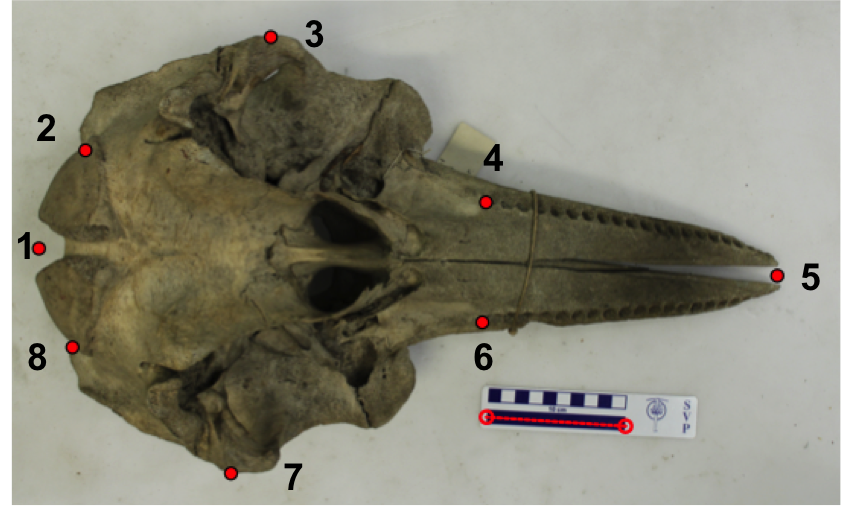
\includegraphics{whale.png}
\caption{Whale landmarks example}
\end{figure}

\begin{enumerate}
\def\labelenumi{\arabic{enumi}.}
\tightlist
\item
  Midway point between the occipital condyles.
\item
  Suture where lacrimojugal and basoccipital bones join on left hand
  side (indentation).
\item
  Most extreme point of the zygomatic arch on left hand side.
\item
  Anterior edge of on rearmost tooth on left hand side.
\item
  Tip of the rostrum.
\item
  Same as 4 but right hand side.
\item
  Same as 3 but right hand side.
\item
  Same as 2 but right hand side.
\end{enumerate}

Digitizing is pretty simple to do in \texttt{geomorph}, though some
people prefer to use package
\href{https://imagej.nih.gov/ij/download.html}{ImageJ} or
\href{http://life.bio.sunysb.edu/morph/soft-dataacq.html}{tpsdig} which
are more user friendly. Either way, you use the mouse to click on the
photos at the point you want each landmark to be. Curves/semi-landmarks
are added after the initial digitisation step. Today we will use
\texttt{geomorph} and we won't add any curves.

Remember you need to add landmarks in the \textbf{same order} for each
specimen, and don't forget to add the \textbf{scale} before you start.
This step can be a time consuming process in a real analysis.

\textbf{You will need to use the normal R Console, NOT RStudio for this
stage to work}

We are going to use the function \texttt{digitize2d} to add eight
landmarks (\texttt{nlandmarks\ =\ 8}) to our list of photos
(\texttt{list.files(pattern\ =\ ".jpg")}) and output these into a TPS
(thin plate spline) file called \texttt{whale\_landmarks.tps}. The scale
bars in each photo are 10cm long so we add \texttt{scale\ =\ 10}.

\begin{Shaded}
\begin{Highlighting}[]
\KeywordTok{digitize2d}\NormalTok{(}\DataTypeTok{filelist =} \KeywordTok{list.files}\NormalTok{(}\DataTypeTok{pattern =} \StringTok{".jpg"}\NormalTok{),}
           \DataTypeTok{nlandmarks =} \DecValTok{8}\NormalTok{, }\DataTypeTok{tpsfile =} \StringTok{"whale_landmarks.tps"}\NormalTok{, }\DataTypeTok{scale =} \DecValTok{10}\NormalTok{)}
\end{Highlighting}
\end{Shaded}

Note that if you stop this procedure and then start again you may get
the following error message:
\texttt{Filelist\ does\ not\ contain\ the\ same\ specimens\ as\ TPS\ file.}
To fix this you just need to delete \texttt{whale\_landmarks.tps} from
your working directory and then start again.

If you don't get an error you should find that a picture of the first
specimen appears in your plotting window, and the message:

\texttt{Only\ 1\ scale\ measure\ provided.\ Will\ use\ scale\ =\ 10\ \ for\ all\ specimens.\ Digitizing\ specimen\ 1\ in\ filelist\ \ Set\ scale\ =\ 10}

To digitize proceed as follows. You will need to repeat this for
\emph{each} photo.

\begin{enumerate}
\def\labelenumi{\arabic{enumi}.}
\tightlist
\item
  Set the scale by clicking on the start and end of the black scale bar.
\item
  The console will then display \texttt{Keep\ scale\ (y/n)?}. If you're
  happy press \texttt{y}, if not press \texttt{n} and try again. The
  function will check you are happy after every landmark you place. This
  gets a bit tedious but means you don't have to start over if you click
  somewhere by accident.
\item
  Select landmark 1, click \texttt{y} when happy, then select landmark 2
  and so on\ldots{}
\item
  Once you've finished one specimen, you'll be asked if you want to
  continue to the next specimen. Again you need to press \texttt{y} to
  continue.
\item
  Continue until all eight are digitised
\end{enumerate}

Each specimen should end up looking something like this once the scale
and landmarks have been added.

\begin{figure}
\centering
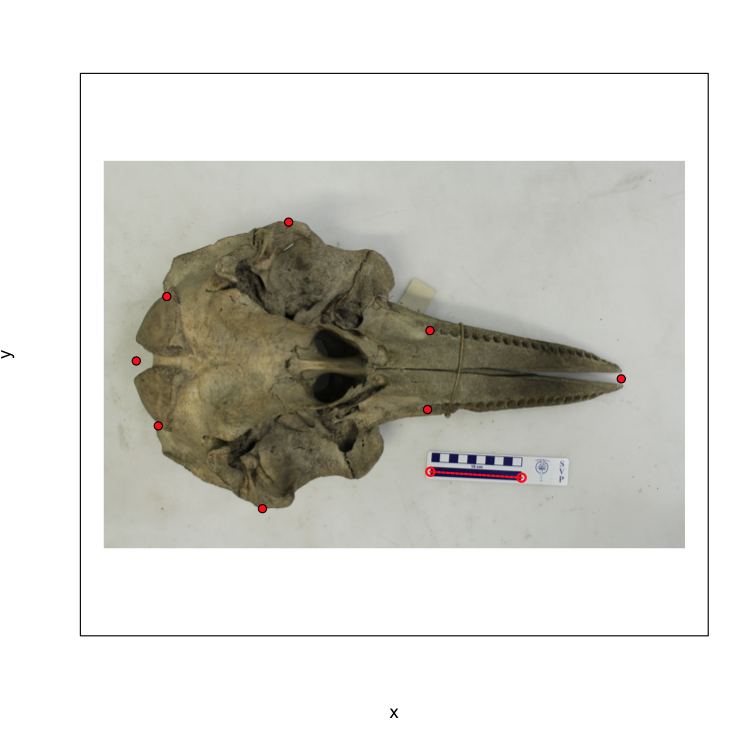
\includegraphics{whale3.png}
\caption{What your photos should look like post digitising}
\end{figure}

Don't get too worried about digitising accurately today. This is just an
example so you get a chance to try this out. You'll notice that some
landmarks are a lot harder than others to place accurately each time,
bringing us back to thinking about potential sources of error.

If you're having trouble with this step you can use the TPS file I made
earlier.

\section{Reading in your data and plotting
it}\label{reading-in-your-data-and-plotting-it}

We can now read in our TPS file to look at our landmarks using
\texttt{readland.tps}. I've asked it to add the specimen identities from
the file names so we know which species is which by using
\texttt{specID\ =\ "ID"}.

\begin{Shaded}
\begin{Highlighting}[]
\NormalTok{landmarks <-}\StringTok{ }\KeywordTok{readland.tps}\NormalTok{(}\StringTok{"whale_landmarks.tps"}\NormalTok{, }\DataTypeTok{specID =} \StringTok{"ID"}\NormalTok{)}
\end{Highlighting}
\end{Shaded}

\begin{verbatim}
## [1] "Specimen names extracted from line ID="
\end{verbatim}

We can look at all the landmarks by typing:

\begin{Shaded}
\begin{Highlighting}[]
\NormalTok{landmarks}
\end{Highlighting}
\end{Shaded}

To save printing them all out I'll just look at the landmarks for the
first specimen (\emph{Pseudorca crassidens}).

\begin{Shaded}
\begin{Highlighting}[]
\NormalTok{landmarks[, , }\DecValTok{1}\NormalTok{]}
\end{Highlighting}
\end{Shaded}

\begin{verbatim}
##           [,1]      [,2]
## [1,]  4.917176 31.136595
## [2,] 16.863048 49.815389
## [3,] 27.883473 60.925151
## [4,] 58.264038 42.370924
## [5,] 82.299223 33.057950
## [6,] 58.449630 19.410289
## [7,] 26.973126  1.064303
## [8,] 16.559808 11.230374
\end{verbatim}

These are the Y and X coordinates of each point \emph{after scaling}.
They are scaled in the units of your scale bar (in the case mm). If you
look at the TPS file itself in a text editor you'll see the numbers are
different and there is information on the length of the scale bars.

We can plot the coordinates for the \emph{Pseudorca} (specimen 1) and
the \emph{Tursiops truncatus} (specimen 8) specimens as follows.

\begin{Shaded}
\begin{Highlighting}[]
\KeywordTok{plot}\NormalTok{(landmarks[, , }\DecValTok{1}\NormalTok{], }\DataTypeTok{pch =} \DecValTok{16}\NormalTok{, }\DataTypeTok{xlab =} \StringTok{"X coordinate"}\NormalTok{, }\DataTypeTok{ylab =} \StringTok{"Y coordinate"}\NormalTok{)}
\KeywordTok{points}\NormalTok{(landmarks[, , }\DecValTok{8}\NormalTok{], }\DataTypeTok{col =} \StringTok{"red"}\NormalTok{, }\DataTypeTok{pch =} \DecValTok{16}\NormalTok{)}
\end{Highlighting}
\end{Shaded}

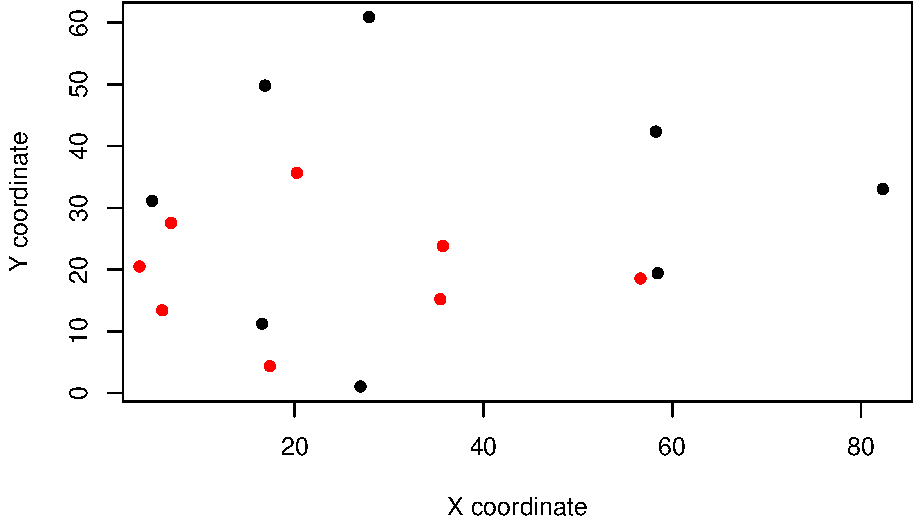
\includegraphics{macro-module_files/figure-latex/unnamed-chunk-146-1.pdf}

You can see that although both filled the screen when you were
digitising, \emph{Tursiops} (in red) is much smaller. This is why this
scaling step is so important.

\section{Generalised Procrustes Superimposition
(GPA)}\label{generalised-procrustes-superimposition-gpa}

If you plot all the landmarks at the same time you'll notice it's a bit
of a mess.

\begin{Shaded}
\begin{Highlighting}[]
\KeywordTok{plot}\NormalTok{(landmarks[, }\DecValTok{2}\NormalTok{, ] ~}\StringTok{ }\NormalTok{landmarks[, }\DecValTok{1}\NormalTok{, ], }\DataTypeTok{xlab =} \StringTok{"X coordinate"}\NormalTok{, }\DataTypeTok{ylab =} \StringTok{"Y coordinate"}\NormalTok{)}
\end{Highlighting}
\end{Shaded}

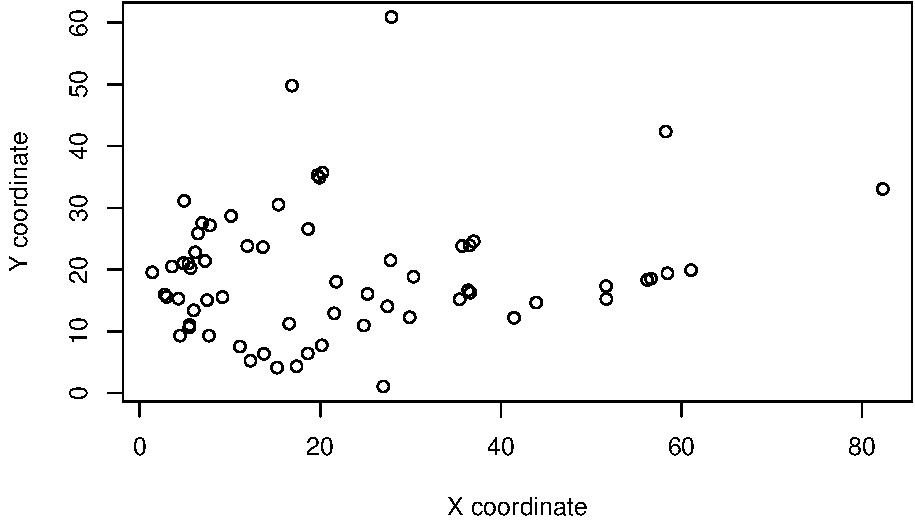
\includegraphics{macro-module_files/figure-latex/unnamed-chunk-147-1.pdf}

The skulls vary in their placement in each photo - in some they cover
the whole area, in others they are further forward or sideways, some are
at a slight angle (rotation). Also as we already noted, there is a
difference in the \emph{size} of the skulls. Remember that we are
interested in comparing shapes and shape is defined as \textbf{the
property of an object invariant under scaling, rotation, or
translation}. So if we want to compare shapes, we need to remove these
differences.

Luckily a number of solutions exist. We are going to use Generalised
Procrustes Superimposition/Analysis (GPA). GPA is a way to remove
rotation, translation and scaling differences among specimens so they
can be compared. GPA translates all specimens to the origin (0,0,0),
scales them to unit-centroid size, and optimally rotates them (using a
least-squares criterion) until the coordinates of corresponding points
align as closely as possible. The resulting aligned Procrustes
coordinates represent the shape of each specimen.

This is hard to explain in words, but there are a number of excellent
graphical explanations in the references below.

Remember that you \emph{never} do a morphometrics analysis on the raw
landmarks, they must always be aligned first or the results are
meaningless. Also remember that you need to align \textbf{all} the
specimens you want to use in your analysis at the same time, or again
your analysis will be meaningless.

To do this in R we just need one line of code and the function
\texttt{gpagen}.

\begin{Shaded}
\begin{Highlighting}[]
\NormalTok{gpa.landmarks <-}\StringTok{ }\KeywordTok{gpagen}\NormalTok{(landmarks)}
\end{Highlighting}
\end{Shaded}

\begin{verbatim}
## 
  |                                                                       
  |                                                                 |   0%
  |                                                                       
  |=============                                                    |  20%
  |                                                                       
  |==========================                                       |  40%
  |                                                                       
  |=================================================================| 100%
\end{verbatim}

\begin{Shaded}
\begin{Highlighting}[]
\CommentTok{# Plot the Procrusted coordinates }
\KeywordTok{plot}\NormalTok{(gpa.landmarks)}
\end{Highlighting}
\end{Shaded}

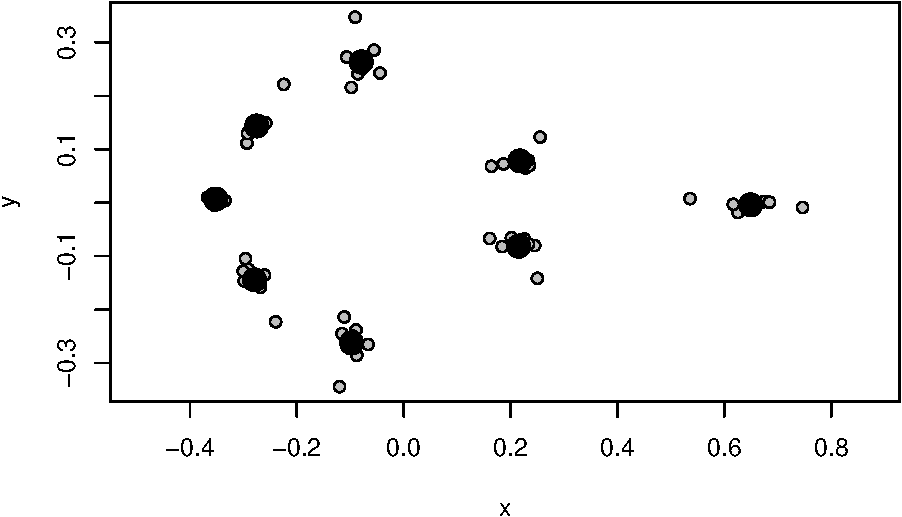
\includegraphics{macro-module_files/figure-latex/unnamed-chunk-148-1.pdf}

Note that now we have the average for each landmark as a large black
point (the \textbf{centroid} - centroid just means the centre point of a
sample of points/shapes), and the aligned landmarks for each specimen
scattered around these in grey. You can see some landmarks are very
variable, while others are more constant across our specimens.

\texttt{gpagen} not only outputs a nice plot of the specimens and their
mean shape, but also the superimposed coordinates (\texttt{\$coords}),
the shape variables as principal components
(\texttt{\$pc.scores)\ and\ the\ centroid\ size\ of\ the\ specimens\ (}Csize`).

\section{Principal components and
plotting}\label{principal-components-and-plotting}

We now have superimposed coordinates we can use to further investigate
shape variation among our specimens. But there's a bit of a problem. If
you think back to the assumptions we make when we do statistics, we
often talk about how the variables should not be correlated. Here our
points are highly correlated, e.g.~the tip of the rostrum can only be in
front of the back of the tooth row, so where the tooth row is in each
specimen will be closely related to where the rostrum tip is. It can
also be a bit hard to interpret analyses with all the landmarks included
- how do we interpret a result that suggests a small increase in rostrum
tip and a decrease in occipital condyle? To solve these issues we can
use principal components analysis (PCA).

PCA finds the axes of greatest variation in a dataset and removes
correlations among variables. It does this while still preserving the
distances between data points - i.e.~it doesn't distort variation in the
data. The outputs of PCA are principal components scores, which we can
think of as ``shape variables''. These PC scores tend to be used in any
further analysis and are \textbf{independent components of shape
variation}. Note that PCA is essentially just a rotation of the data,
nothing more complicated than that. Again I recommend checking out the
graphical examples in the texts below to help with your understanding.

Let's extract principal components scores for our cetacean dataset using
\texttt{plotTangentSpace}.

\begin{Shaded}
\begin{Highlighting}[]
\NormalTok{pca.landmarks <-}\StringTok{ }\KeywordTok{plotTangentSpace}\NormalTok{(gpa.landmarks$coords, }\DataTypeTok{label =} \OtherTok{TRUE}\NormalTok{)}
\end{Highlighting}
\end{Shaded}

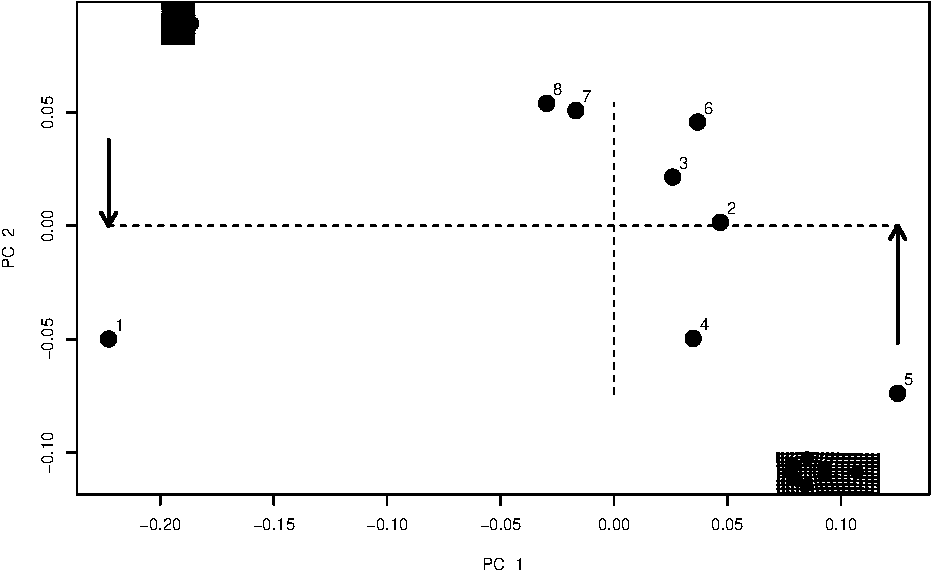
\includegraphics{macro-module_files/figure-latex/unnamed-chunk-149-1.pdf}
This produces a plot of the first two principal components (PC1 and
PC2), with dotted lines at the origin and each specimen represented by a
point. Point 1 is \emph{Pseudorca}. Note that what we are now looking at
is called a ``shape space'' or ``morphospace''. \textbf{Each point
represents a shape} not an individual landmark.

To help with interpretation, two grids are also plotted. These represent
the shape at the points indicated by the arrows. These are called thin
plate splines, because we imagine the landmarks for the average/centroid
shape were engraved on a thin plate of metal, and then deformed to get
to the shapes at the indicated points. The grid to the left shows lots
of deformation, with a widening of the back of the skull, and a
shortening of the rostrum. The grid to the right shows deformation with
the tooth rows being closer together and some stretching at the front to
enlarge the rostrum. Specimens with high PC1 scores look more like the
right hand grid, specimens with low PC1 scores look more like the left
hand grid.

We can look at these grids individually, and for the other PC axes. The
code below will show us the grids for the min and max PC1 and PC2. Note
that I have included \texttt{mag\ =\ 2} which magnifies the differences
two fold to make them easier to see.

\begin{Shaded}
\begin{Highlighting}[]
\CommentTok{# Make plotting window into 2 x 2 grid}
\KeywordTok{par}\NormalTok{(}\DataTypeTok{mfrow =} \KeywordTok{c}\NormalTok{(}\DecValTok{2}\NormalTok{, }\DecValTok{2}\NormalTok{))}
\CommentTok{# Reduce margins around the plots}
\KeywordTok{par}\NormalTok{(}\DataTypeTok{mar =} \KeywordTok{c}\NormalTok{(}\DecValTok{0}\NormalTok{, }\DecValTok{0}\NormalTok{, }\DecValTok{0}\NormalTok{, }\DecValTok{0}\NormalTok{))}

\CommentTok{# Select reference shape - the centroid of our Procrustes aligned coordinates}
\NormalTok{ref <-}\StringTok{ }\KeywordTok{mshape}\NormalTok{(gpa.landmarks$coords)}

\CommentTok{# Plot each min/max PC scores in comparison to the reference shape (ref) }
\CommentTok{# with two fold magnification (mag = 2)}
\KeywordTok{plotRefToTarget}\NormalTok{(ref, pca.landmarks$pc.shapes$PC1min, }\DataTypeTok{mag =} \DecValTok{2}\NormalTok{)}
\KeywordTok{plotRefToTarget}\NormalTok{(ref, pca.landmarks$pc.shapes$PC1max, }\DataTypeTok{mag =} \DecValTok{2}\NormalTok{)}
\KeywordTok{plotRefToTarget}\NormalTok{(ref, pca.landmarks$pc.shapes$PC2min, }\DataTypeTok{mag =} \DecValTok{2}\NormalTok{)}
\KeywordTok{plotRefToTarget}\NormalTok{(ref, pca.landmarks$pc.shapes$PC2max, }\DataTypeTok{mag =} \DecValTok{2}\NormalTok{)}
\end{Highlighting}
\end{Shaded}

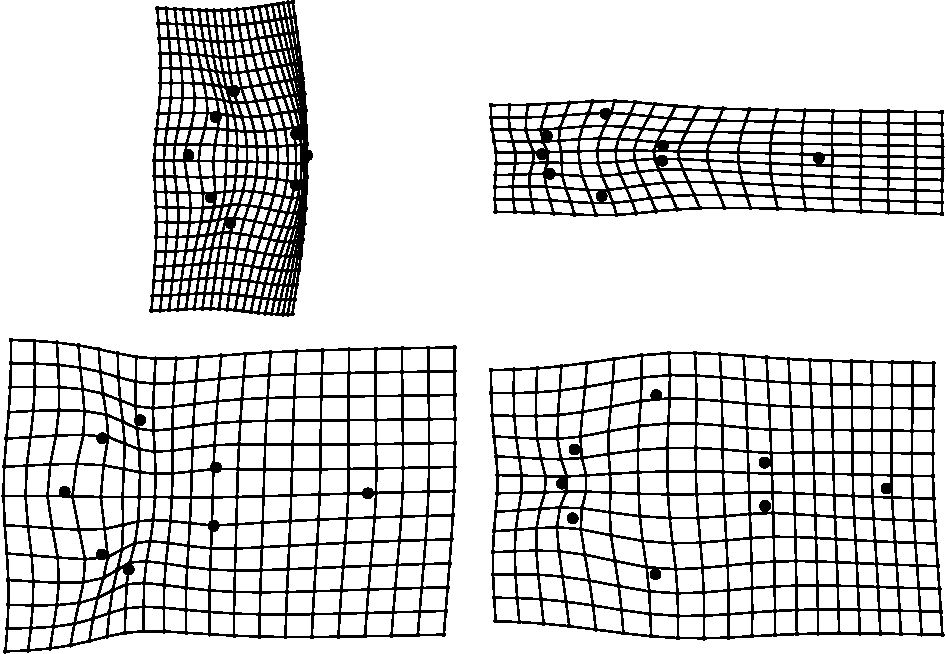
\includegraphics{macro-module_files/figure-latex/unnamed-chunk-150-1.pdf}

\begin{Shaded}
\begin{Highlighting}[]
\CommentTok{# Put graphics parameters back to default settings}
\KeywordTok{par}\NormalTok{(}\DataTypeTok{mfrow =} \KeywordTok{c}\NormalTok{(}\DecValTok{2}\NormalTok{, }\DecValTok{2}\NormalTok{))}
\KeywordTok{par}\NormalTok{(}\DataTypeTok{mar =} \KeywordTok{c}\NormalTok{(}\DecValTok{5}\NormalTok{, }\DecValTok{4}\NormalTok{, }\DecValTok{4}\NormalTok{, }\DecValTok{2}\NormalTok{))}
\end{Highlighting}
\end{Shaded}

Another way of interpreting PC scores is to extract the
\textbf{loadings} for each PC using \texttt{\$rotation}.

\begin{Shaded}
\begin{Highlighting}[]
\NormalTok{pca.landmarks$rotation}
\end{Highlighting}
\end{Shaded}

\begin{verbatim}
##               PC1         PC2          PC3         PC4         PC5
##  [1,]  0.07782421  0.01145886  0.010978946 -0.12118065  0.32956627
##  [2,] -0.01685081 -0.02976881  0.237243510  0.15913484 -0.24917185
##  [3,] -0.15165444 -0.35228327  0.131087366 -0.10282307 -0.11148058
##  [4,] -0.26942003 -0.35780565  0.109069813  0.24333031  0.05325473
##  [5,]  0.02198347  0.09012823 -0.784843674  0.20706328 -0.32689443
##  [6,] -0.38619090  0.02990721 -0.053598578 -0.37241810 -0.21857694
##  [7,] -0.23106590  0.32574319  0.026774344  0.21696513  0.37957940
##  [8,] -0.16544042 -0.11557074 -0.153305579 -0.15718351  0.22318585
##  [9,]  0.57879930 -0.30554975  0.024395464 -0.13850038  0.01307704
## [10,] -0.03727420 -0.06838202 -0.212667343  0.08987931 -0.04242125
## [11,] -0.23534726  0.36264877  0.184749068  0.19886767  0.17186361
## [12,]  0.23024040  0.16755749 -0.072168034  0.17366534 -0.03227954
## [13,]  0.02898251  0.23494160  0.398172339 -0.04393459 -0.61107235
## [14,]  0.37752351 -0.03750461  0.165149456  0.42261250  0.12908818
## [15,] -0.08952190 -0.36708762  0.008686147 -0.21645738  0.15536103
## [16,]  0.26741245  0.41156713 -0.019723245 -0.55902070  0.13692083
##                PC6         PC7         PC8
##  [1,]  0.732980006 -0.08204786 -0.14042273
##  [2,] -0.034715583  0.36122405 -0.05381482
##  [3,]  0.007281487  0.43550615  0.06763819
##  [4,]  0.158610967 -0.27638033  0.52594604
##  [5,] -0.041646343 -0.07954720  0.05088173
##  [6,]  0.149383964 -0.19916231 -0.56878480
##  [7,] -0.128169667  0.36715675 -0.20297068
##  [8,] -0.023489409 -0.04840285  0.04503906
##  [9,]  0.054086438  0.03069426 -0.12319514
## [10,]  0.037088383  0.41908435 -0.10530240
## [11,] -0.117978102 -0.24845750  0.03602596
## [12,]  0.071908482 -0.21206921 -0.03395509
## [13,]  0.045527030 -0.13851486  0.01994870
## [14,] -0.161022728 -0.14265102 -0.34854652
## [15,] -0.552080849 -0.28478974 -0.20316407
## [16,] -0.197764076  0.09835732  0.36740417
\end{verbatim}

This shows how each of our landmarks contributes to each PC. Larger
numbers mean the landmark has more influence on the PC, negative numbers
show a negative effect. These can be hard to interpret but worth looking
at. Remember each landmark has an X and a Y coordinate, so
\texttt{{[}1,{]}} is the X coordinate of the occipital condyle landmark,
and \texttt{{[}2,{]}} is the Y coordinate.

Here for example I'd suggest that PC1 is most heavily influenced by
\texttt{{[}9,{]}}, the X coordinate of landmark 5, the tip of the
rostrum. It's a positive number so it means species with high values for
PC1 have an elongated rostrum. See if you can interpret these results
further. It is often best to look at the loadings and the plots above to
help with this.

Another important output to look at is the summary of the PC axes:

\begin{Shaded}
\begin{Highlighting}[]
\KeywordTok{summary}\NormalTok{(pca.landmarks)}
\end{Highlighting}
\end{Shaded}

\begin{verbatim}
## 
## PC Summary
## 
## Importance of components:
##                           PC1     PC2     PC3     PC4     PC5      PC6
## Standard deviation     0.1013 0.05135 0.02514 0.01454 0.01177 0.006117
## Proportion of Variance 0.7361 0.18906 0.04531 0.01517 0.00994 0.002680
## Cumulative Proportion  0.7361 0.92521 0.97052 0.98568 0.99562 0.998300
##                             PC7       PC8
## Standard deviation     0.004865 2.022e-17
## Proportion of Variance 0.001700 0.000e+00
## Cumulative Proportion  1.000000 1.000e+00
\end{verbatim}

This shows the variance on each PC axis (eigenvalues). Note that the
first PC has the highest proportion of the variance (73.61\%). PCs will
always decrease in the amount of variance explained because of the way
PCA works - it takes the axis that explains most variation first. Often
people will only use PCs in their later analyses that sum up to 95\% or
99\% of the cumulative variance, because the later PCs are not really
explaining much of the variation in shapes. In this example we'd
probably use PC1, PC2 and PC3.

Finally, to extract the PC scores for each specimen we use
\texttt{\$pc.scores}. We'll use these for all further analysis.

\begin{Shaded}
\begin{Highlighting}[]
\NormalTok{pca.landmarks$pc.scores}
\end{Highlighting}
\end{Shaded}

\begin{verbatim}
##                                               PC1         PC2
## Pseudorca_crassidens_1961.6.14.3.jpg  -0.22279912 -0.04990209
## Sousa_plumbea_70.1506.jpg              0.04682774  0.00149044
## Stenella_attenuata_1960.6.24.1.jpg     0.02583791  0.02145984
## Stenella_coeruleoalba_1938.2.5.1.jpg   0.03489668 -0.04967601
## Stenella_longirostris_1965.8.25.2.jpg  0.12500666 -0.07385256
## Steno_bredanensis_345c.jpg             0.03680834  0.04572532
## Tursiops_aduncus_1903.9.12.1.jpg      -0.01687868  0.05079845
## Tursiops_truncatus_1920.8.14.1.jpg    -0.02969952  0.05395661
##                                                 PC3          PC4
## Pseudorca_crassidens_1961.6.14.3.jpg  -0.0006377733 -0.001028733
## Sousa_plumbea_70.1506.jpg             -0.0417508568  0.009805947
## Stenella_attenuata_1960.6.24.1.jpg     0.0169424424  0.030573421
## Stenella_coeruleoalba_1938.2.5.1.jpg   0.0008958266  0.001192135
## Stenella_longirostris_1965.8.25.2.jpg  0.0118958174 -0.010838289
## Steno_bredanensis_345c.jpg            -0.0043676504 -0.014536311
## Tursiops_aduncus_1903.9.12.1.jpg       0.0408120527 -0.006280211
## Tursiops_truncatus_1920.8.14.1.jpg    -0.0237898587 -0.008887959
##                                                PC5           PC6
## Pseudorca_crassidens_1961.6.14.3.jpg   0.006797670 -7.155469e-05
## Sousa_plumbea_70.1506.jpg              0.004444909 -8.639956e-03
## Stenella_attenuata_1960.6.24.1.jpg     0.004876528  5.166614e-03
## Stenella_coeruleoalba_1938.2.5.1.jpg  -0.023181651 -2.208889e-03
## Stenella_longirostris_1965.8.25.2.jpg  0.009562895  4.327237e-03
## Steno_bredanensis_345c.jpg             0.011629308 -1.185434e-03
## Tursiops_aduncus_1903.9.12.1.jpg      -0.004195661 -6.823983e-03
## Tursiops_truncatus_1920.8.14.1.jpg    -0.009933998  9.435965e-03
##                                                 PC7          PC8
## Pseudorca_crassidens_1961.6.14.3.jpg   0.0003870485 0.000000e+00
## Sousa_plumbea_70.1506.jpg             -0.0036414119 2.081668e-17
## Stenella_attenuata_1960.6.24.1.jpg     0.0017329304 2.059984e-17
## Stenella_coeruleoalba_1938.2.5.1.jpg   0.0049957672 1.387779e-17
## Stenella_longirostris_1965.8.25.2.jpg -0.0037522008 2.992398e-17
## Steno_bredanensis_345c.jpg             0.0086445940 3.122502e-17
## Tursiops_aduncus_1903.9.12.1.jpg      -0.0046789921 1.908196e-17
## Tursiops_truncatus_1920.8.14.1.jpg    -0.0036877353 2.341877e-17
\end{verbatim}

\section{Statistical analyses of geometric morphometric
datasets}\label{statistical-analyses-of-geometric-morphometric-datasets}

This is the point at which geometric morphometrics gets really exciting
- it's the point that you get to answer whatever question you started
out with! It's also the point at which the number of different options
becomes very large. Two common analyses are regressions and multivariate
ANOVA (MANOVA). Regressions are used when you have continuous
explanatory variables, for example if you want to see if body size is
correlated with shape. MANOVA (or ANOVA) is used when you have
categorical explanatory variables, for example if you want to see if
habitat type is correlated with shape.

At this stage of the analysis we often add a new dataset containing our
variables of interest. For simplicity we will just invent some data as
follows.

\begin{Shaded}
\begin{Highlighting}[]
\CommentTok{# Create new dataframe with PC scores, body size and diet.}
\CommentTok{# Body sizes from a random normal distribution with mean of 100 and sd of 25.}
\CommentTok{# Diet assigned as squid to first two specimens and fish to others.}
\NormalTok{mydata <-}\StringTok{ }\KeywordTok{data.frame}\NormalTok{(pca.landmarks$pc.scores, }
                     \DataTypeTok{body.size =} \KeywordTok{rnorm}\NormalTok{(}\DataTypeTok{n =} \DecValTok{8}\NormalTok{, }\DataTypeTok{mean =} \DecValTok{100}\NormalTok{, }\DataTypeTok{sd =} \DecValTok{25}\NormalTok{), }
                     \DataTypeTok{diet =} \KeywordTok{c}\NormalTok{(}\KeywordTok{rep}\NormalTok{(}\StringTok{"squid"}\NormalTok{,}\DecValTok{2}\NormalTok{), }\KeywordTok{rep}\NormalTok{(}\StringTok{"fish"}\NormalTok{, }\DecValTok{6}\NormalTok{)) }
                     \NormalTok{)}
\CommentTok{# Look at the data}
\KeywordTok{str}\NormalTok{(mydata)}
\end{Highlighting}
\end{Shaded}

\begin{verbatim}
## 'data.frame':    8 obs. of  10 variables:
##  $ PC1      : num  -0.2228 0.0468 0.0258 0.0349 0.125 ...
##  $ PC2      : num  -0.0499 0.00149 0.02146 -0.04968 -0.07385 ...
##  $ PC3      : num  -0.000638 -0.041751 0.016942 0.000896 0.011896 ...
##  $ PC4      : num  -0.00103 0.00981 0.03057 0.00119 -0.01084 ...
##  $ PC5      : num  0.0068 0.00444 0.00488 -0.02318 0.00956 ...
##  $ PC6      : num  -7.16e-05 -8.64e-03 5.17e-03 -2.21e-03 4.33e-03 ...
##  $ PC7      : num  0.000387 -0.003641 0.001733 0.004996 -0.003752 ...
##  $ PC8      : num  0.00 2.08e-17 2.06e-17 1.39e-17 2.99e-17 ...
##  $ body.size: num  109.7 119.1 124.1 95.7 90.3 ...
##  $ diet     : Factor w/ 2 levels "fish","squid": 2 2 1 1 1 1 1 1
\end{verbatim}

\section{Regression}\label{regression}

Regressions are done in the same way as usual.

\begin{Shaded}
\begin{Highlighting}[]
\CommentTok{# Fit model}
\NormalTok{model1 <-}\StringTok{ }\KeywordTok{lm}\NormalTok{(PC1 ~}\StringTok{ }\NormalTok{body.size, }\DataTypeTok{data =} \NormalTok{mydata)}

\CommentTok{# Assess assumptions}
\KeywordTok{par}\NormalTok{(}\DataTypeTok{mfrow =} \KeywordTok{c}\NormalTok{(}\DecValTok{2}\NormalTok{,}\DecValTok{2}\NormalTok{))}
\KeywordTok{plot}\NormalTok{(model1)}
\end{Highlighting}
\end{Shaded}

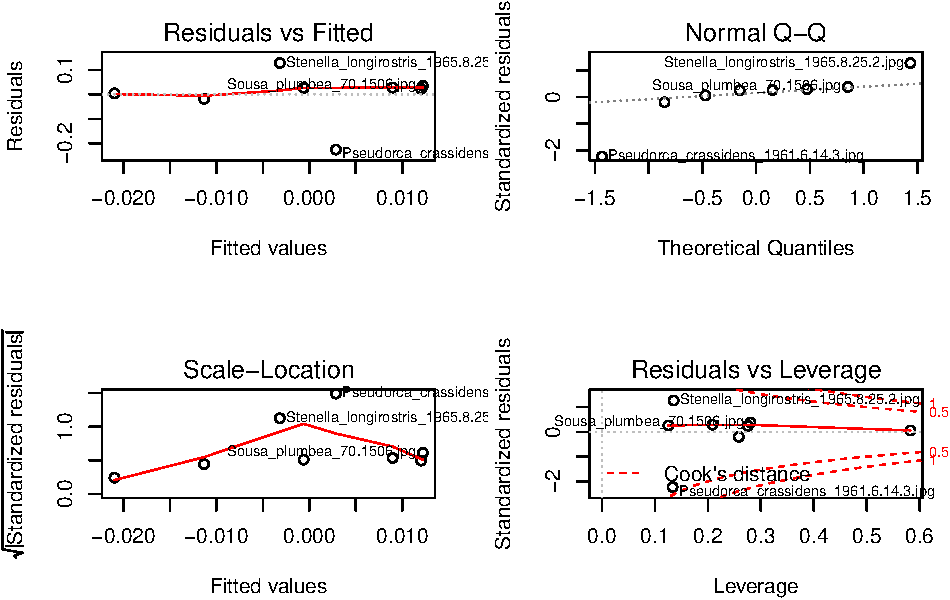
\includegraphics{macro-module_files/figure-latex/unnamed-chunk-155-1.pdf}

\begin{Shaded}
\begin{Highlighting}[]
\KeywordTok{par}\NormalTok{(}\DataTypeTok{mfrow =} \KeywordTok{c}\NormalTok{(}\DecValTok{1}\NormalTok{,}\DecValTok{1}\NormalTok{))}

\CommentTok{# Look at overall model significance}
\KeywordTok{anova}\NormalTok{(model1)}
\end{Highlighting}
\end{Shaded}

\begin{verbatim}
## Analysis of Variance Table
## 
## Response: PC1
##           Df   Sum Sq   Mean Sq F value Pr(>F)
## body.size  1 0.006894 0.0068945  0.6367 0.4553
## Residuals  6 0.064972 0.0108286
\end{verbatim}

\begin{Shaded}
\begin{Highlighting}[]
\CommentTok{# Look at parameters and their significance}
\KeywordTok{summary}\NormalTok{(model1)}
\end{Highlighting}
\end{Shaded}

\begin{verbatim}
## 
## Call:
## lm(formula = PC1 ~ body.size, data = mydata)
## 
## Residuals:
##      Min       1Q   Median       3Q      Max 
## -0.21765 -0.01125  0.01170  0.06156  0.09248 
## 
## Coefficients:
##              Estimate Std. Error t value Pr(>|t|)
## (Intercept)  0.207250   0.262327   0.790    0.460
## body.size   -0.001936   0.002426  -0.798    0.455
## 
## Residual standard error: 0.1041 on 6 degrees of freedom
## Multiple R-squared:  0.09593,    Adjusted R-squared:  -0.05474 
## F-statistic: 0.6367 on 1 and 6 DF,  p-value: 0.4553
\end{verbatim}

\begin{Shaded}
\begin{Highlighting}[]
\CommentTok{# Plot}
\KeywordTok{plot}\NormalTok{(PC1 ~}\StringTok{ }\NormalTok{body.size, }\DataTypeTok{data =} \NormalTok{mydata, }\DataTypeTok{pch =} \DecValTok{16}\NormalTok{)}
\KeywordTok{abline}\NormalTok{(model1)}
\end{Highlighting}
\end{Shaded}

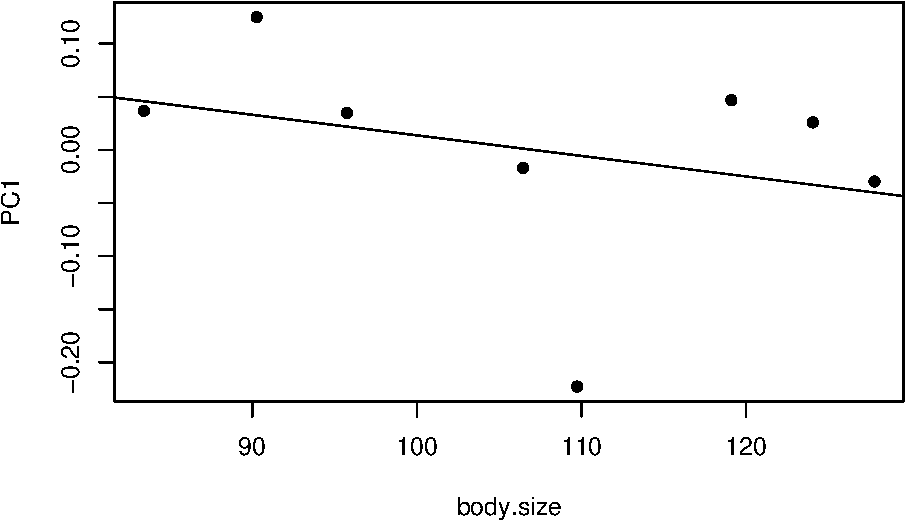
\includegraphics{macro-module_files/figure-latex/unnamed-chunk-155-2.pdf}

\begin{itemize}
\tightlist
\item
  Can you remember how to interpret these results?
\item
  Why will your results be different to mine?
\end{itemize}

\section{Multivariate regression}\label{multivariate-regression}

Multivariate regression is the same as univariate regression but is used
where you have multiple response variables, i.e.~if we wanted to include
PC1 and PC2 in the analysis. It's quite easy to implement, we just use
\texttt{cbind} to bind together the different variables we want to
include. Note that assumption checking isn't possible, nor is plotting
in the usual way. Additionally, \texttt{summary(model)} presents the
parameters for each response variable separately (e.g.
\texttt{PC1\ \textasciitilde{}\ body.size} then
\texttt{PC2\ \textasciitilde{}\ body.size}) so is not particularly
useful here.

\begin{Shaded}
\begin{Highlighting}[]
\CommentTok{# Fit model}
\NormalTok{model2 <-}\StringTok{ }\KeywordTok{lm}\NormalTok{(}\KeywordTok{cbind}\NormalTok{(mydata$PC1,mydata$PC2) ~}\StringTok{ }\NormalTok{body.size, }\DataTypeTok{data =} \NormalTok{mydata)}

\CommentTok{# Look at overall model significance}
\KeywordTok{anova}\NormalTok{(model2)}
\end{Highlighting}
\end{Shaded}

\begin{verbatim}
## Analysis of Variance Table
## 
##             Df  Pillai approx F num Df den Df Pr(>F)
## (Intercept)  1 0.00000  0.00000      2      5 1.0000
## body.size    1 0.22067  0.70788      2      5 0.5362
## Residuals    6
\end{verbatim}

\begin{itemize}
\tightlist
\item
  Can you guess how to interpret these results given what you know about
  regression?
\end{itemize}

\section{ANOVA}\label{anova}

ANOVAs are done in the same way as usual.

\begin{Shaded}
\begin{Highlighting}[]
\CommentTok{# Fit model}
\NormalTok{model3 <-}\StringTok{ }\KeywordTok{lm}\NormalTok{(PC1 ~}\StringTok{ }\NormalTok{diet, }\DataTypeTok{data =} \NormalTok{mydata)}

\CommentTok{# Assess assumptions}
\KeywordTok{par}\NormalTok{(}\DataTypeTok{mfrow =} \KeywordTok{c}\NormalTok{(}\DecValTok{2}\NormalTok{,}\DecValTok{2}\NormalTok{))}
\KeywordTok{plot}\NormalTok{(model3)}
\end{Highlighting}
\end{Shaded}

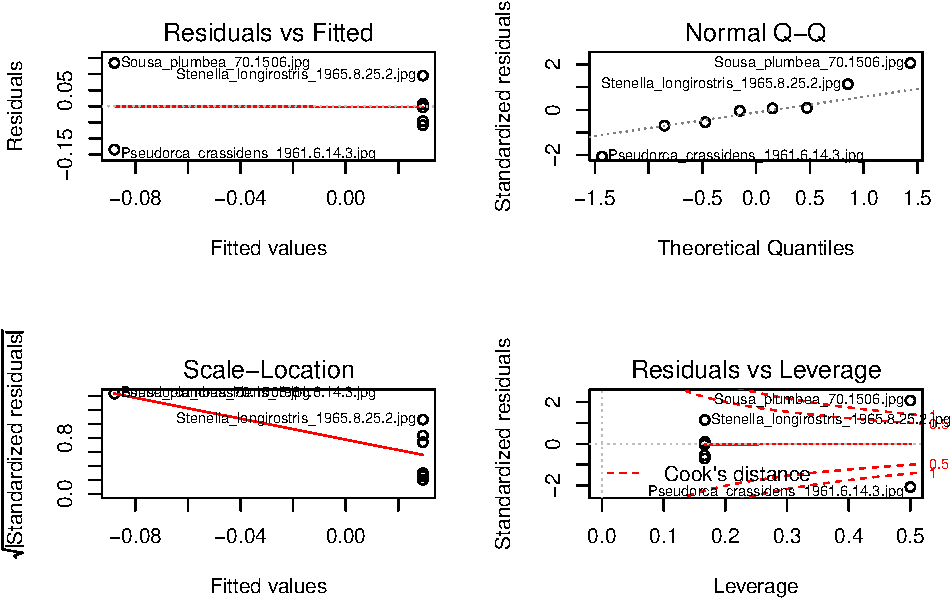
\includegraphics{macro-module_files/figure-latex/unnamed-chunk-157-1.pdf}

\begin{Shaded}
\begin{Highlighting}[]
\KeywordTok{par}\NormalTok{(}\DataTypeTok{mfrow =} \KeywordTok{c}\NormalTok{(}\DecValTok{1}\NormalTok{,}\DecValTok{1}\NormalTok{))}

\CommentTok{# Look at overall model significance}
\KeywordTok{anova}\NormalTok{(model3)}
\end{Highlighting}
\end{Shaded}

\begin{verbatim}
## Analysis of Variance Table
## 
## Response: PC1
##           Df   Sum Sq  Mean Sq F value Pr(>F)
## diet       1 0.020644 0.020644  2.4182 0.1709
## Residuals  6 0.051222 0.008537
\end{verbatim}

\begin{Shaded}
\begin{Highlighting}[]
\CommentTok{# Look at parameters and their significance}
\KeywordTok{summary}\NormalTok{(model3)}
\end{Highlighting}
\end{Shaded}

\begin{verbatim}
## 
## Call:
## lm(formula = PC1 ~ diet, data = mydata)
## 
## Residuals:
##       Min        1Q    Median        3Q       Max 
## -0.134813 -0.049412  0.001039  0.029529  0.134813 
## 
## Coefficients:
##             Estimate Std. Error t value Pr(>|t|)
## (Intercept)  0.02933    0.03772   0.778    0.466
## dietsquid   -0.11731    0.07544  -1.555    0.171
## 
## Residual standard error: 0.0924 on 6 degrees of freedom
## Multiple R-squared:  0.2873, Adjusted R-squared:  0.1685 
## F-statistic: 2.418 on 1 and 6 DF,  p-value: 0.1709
\end{verbatim}

\begin{Shaded}
\begin{Highlighting}[]
\CommentTok{# Plot}
\KeywordTok{plot}\NormalTok{(PC1 ~}\StringTok{ }\NormalTok{diet, }\DataTypeTok{data =} \NormalTok{mydata, }\DataTypeTok{col =} \KeywordTok{c}\NormalTok{(}\StringTok{"lightblue"}\NormalTok{, }\StringTok{"springgreen"}\NormalTok{))}
\end{Highlighting}
\end{Shaded}

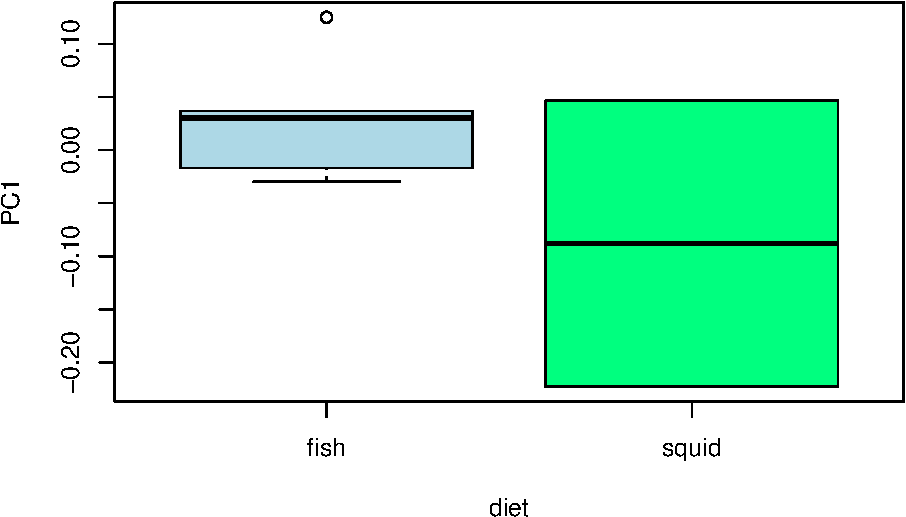
\includegraphics{macro-module_files/figure-latex/unnamed-chunk-157-2.pdf}

\begin{itemize}
\tightlist
\item
  Can you remember how to interpret these results?
\end{itemize}

\section{MANOVA}\label{manova}

MANOVA is the same as ANOVA but is used where you have multiple response
variables, i.e.~if we wanted to include PC1 and PC2 in the analysis.
It's quite easy to implement, we just use \texttt{cbind} to bind
together the different variables we want to include. Note that
assumption checking isn't possible for MANOVA in R at this time.

\begin{Shaded}
\begin{Highlighting}[]
\CommentTok{# Fit model}
\NormalTok{model4 <-}\StringTok{ }\KeywordTok{manova}\NormalTok{(}\KeywordTok{cbind}\NormalTok{(mydata$PC1,mydata$PC2) ~}\StringTok{ }\NormalTok{diet, }\DataTypeTok{data =} \NormalTok{mydata)}

\CommentTok{# Look at overall model significance}
\KeywordTok{anova}\NormalTok{(model4)}
\end{Highlighting}
\end{Shaded}

\begin{verbatim}
## Analysis of Variance Table
## 
##             Df  Pillai approx F num Df den Df Pr(>F)
## (Intercept)  1 0.00000   0.0000      2      5 1.0000
## diet         1 0.37191   1.4803      2      5 0.3127
## Residuals    6
\end{verbatim}

\begin{Shaded}
\begin{Highlighting}[]
\CommentTok{# Look at parameters and their significance}
\KeywordTok{summary}\NormalTok{(model4)}
\end{Highlighting}
\end{Shaded}

\begin{verbatim}
##           Df  Pillai approx F num Df den Df Pr(>F)
## diet       1 0.37191   1.4803      2      5 0.3127
## Residuals  6
\end{verbatim}

\begin{Shaded}
\begin{Highlighting}[]
\CommentTok{# Plot }
\KeywordTok{plot}\NormalTok{(}\KeywordTok{cbind}\NormalTok{(mydata$PC1,mydata$PC2) ~}\StringTok{ }\NormalTok{diet, }\DataTypeTok{data =} \NormalTok{mydata, }\DataTypeTok{col =} \KeywordTok{c}\NormalTok{(}\StringTok{"lightblue"}\NormalTok{, }\StringTok{"springgreen"}\NormalTok{))}
\end{Highlighting}
\end{Shaded}

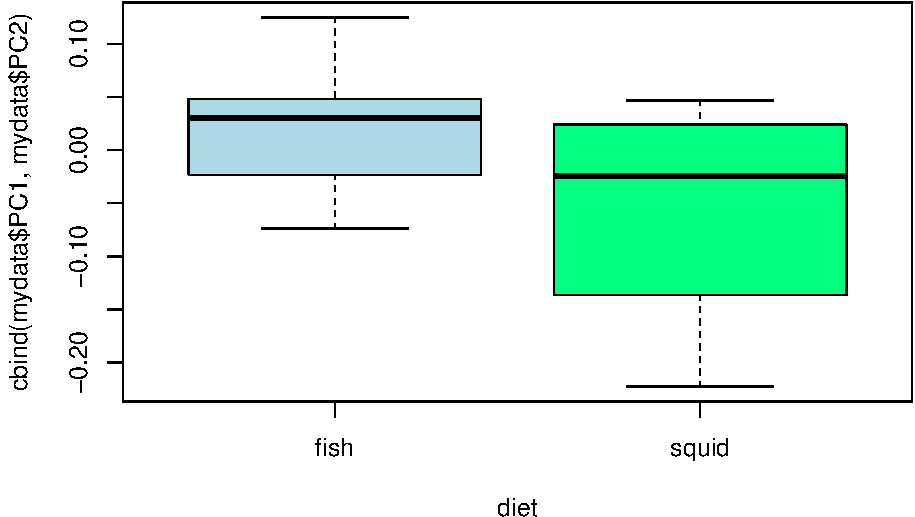
\includegraphics{macro-module_files/figure-latex/unnamed-chunk-158-1.pdf}

\begin{itemize}
\tightlist
\item
  Can you guess how to interpret these results given what you know about
  ANOVA?
\end{itemize}

Of course the results here are nonsensical as we made u pthe data, but
hopefully this gives you an idea of how we might use geometric
morphometrics data in analyses. Other common analyses look at disparity
of groups, convergence and divergence, evolution of shape and shape
space etc.

\begin{center}\rule{0.5\linewidth}{\linethickness}\end{center}

\section{Resources for learning geometric
morphometrics}\label{resources-for-learning-geometric-morphometrics}

\begin{enumerate}
\def\labelenumi{\arabic{enumi}.}
\item
  I highly advise getting hold of this book
  (\href{http://store.elsevier.com/Geometric-Morphometrics-for-Biologists/Miriam-Zelditch/isbn-9780123869036/}{Zelditch
  et al. 2012}) from the library and reading the first few chapters,
  plus any chapters later in the book that are relevant to the analyses
  you will be doing. Don't panic too much about the maths or the
  equations, just try to get a general understanding of what each method
  is doing, especially GPA and PCA.
\item
  Another useful book is
  \href{http://lib.du.ac.ir/documents/10157/60743/Morphometrics+With+R.pdf}{Morphometrics
  with R} by Julien Claude. It is a little harder to read than Zelditch,
  but more focused on practical analysis in R. Note that I'd generally
  advise using the
  \href{https://cran.r-project.org/web/packages/geomorph/geomorph.pdf}{geomorph}
  package (see links below) to do these analyses in R, but many of the
  principles are the same in this book which uses other methods. It's
  available as a
  \href{http://lib.du.ac.ir/documents/10157/60743/Morphometrics+With+R.pdf}{PDF}.
\item
  David Polly has an excellent \href{http://www.indiana.edu/~g562/}{set
  of lectures} about all basic topics in geometric morphometrics
  including PCA and GPA. Note that these use Mathematica not R. There
  are also slides \href{http://www.indiana.edu/~g562/PBDB2013/}{here}
  from an R based course with a basic workflow for an
  \href{http://www.indiana.edu/~g562/PBDB2013/Day\%202B\%20-\%20Geometric\%20Morphometrics\%20in\%20R.pdf}{analysis
  using geomorph}. I'd recommend starting any project with a quick flick
  through these
  \href{http://www.indiana.edu/~g562/PBDB2013/Day\%202A\%20-\%20Introduction\%20to\%20Geometric\%20Morphometrics.pdf}{intro
  slides}
\item
  Emma Sherratt has put together an excellent tutorial/vignette for
  \href{http://www.public.iastate.edu/~dcadams/PDFPubs/Quick\%20Guide\%20to\%20Geomorph\%20v2.0.pdf}{geomorph}
  from inputting landmarks to complex analyses.
\item
  The
  \href{https://cran.r-project.org/web/packages/geomorph/geomorph.pdf}{geomorph
  vignette} may also be helpful for more complex analyses.
\item
  For error checking, take a look at
  \href{http://link.springer.com/article/10.1007/s00427-016-0537-4}{Fruciano
  2016}, a review of the subject in Evolution. Also take a look at
  \href{http://lib.du.ac.ir/documents/10157/60743/Morphometrics+With+R.pdf}{Claude}
  pages 63-65 for ideas on sources of error.
\end{enumerate}

\section{References}\label{references-4}

\begin{itemize}
\tightlist
\item
  Zelditch, M.L., Swiderski, D.L., and Sheets, H.D.. 2012. Geometric
  Morphometrics for Biologists: A Primer. Academic Press.
\item
  Claude, Julien. Morphometrics with R. Springer Science \& Business
  Media, 2008.
\item
  Fruciano, C. Measurement error in geometric morphometrics. 2016.
  Development genes and evolution 226:139-158.
\end{itemize}


\end{document}
